\documentclass[12pt,letterpaper]{report}

\usepackage{amsfonts}
\usepackage{amsmath}
\usepackage{amssymb}
\usepackage{apacite}
\usepackage{caption}
\usepackage{color}
\usepackage{enumitem}
\usepackage{epsfig}
\usepackage{framed}
\usepackage[letterpaper, margin=1in]{geometry}		% Margins should be 1 inch according to McGill requirements (https://www.mcgill.ca/gps/thesis/guidelines/preparation)
\usepackage{graphicx}
\usepackage{listings}
\usepackage{placeins}
\usepackage{setspace}
\usepackage{subcaption}

%%
\newtheorem{lemma}{{\bf Lema}}[chapter]
\newtheorem{theorem}{{\bf Teorema}}[chapter]
\newtheorem{corollary}{{\bf Corolario}}[theorem]
\newtheorem{definition}{{\bf Definici\'on}}[chapter]
\newtheorem{propo}{{\bf Proposicion}}[chapter]

%%
\renewcommand{\vec}[1]{\mbox{$\,${\bf #1}}}
\newcommand{\C}{\mbox{$\mbox{l}\!\!\!\mbox{C}$}}
\newcommand{\N}{\mbox{$\mbox{I}\!\mbox{N}$}}
\newcommand{\R}{\mbox{$\mbox{I}\!\mbox{R}$}}
\newcommand{\Z}{\mbox{$\mbox{Z}\!\!\mbox{Z}$}}
\newcommand{\Rn}{\mbox{$\R^n\,$}}
\newcommand{\Rnxn}{\mbox{$\R^{n \times n}$}}
\newcommand{\Rnxm}{\mbox{$\R^{n \times m}$}}
\newcommand{\Rmxn}{\mbox{$\R^{m \times n}$}}
\newcommand{\Rmxm}{\mbox{$\R^{m \times m}$}}
\newcommand{\inertia}[1]{\mbox{$\cal I$($#1$)}}
\newcommand{\ceil}[1]{\mbox{$\left\lceil #1 \right\rceil$}}
\newcommand{\floor}[1]{\mbox{$\left\lfloor #1 \right\rfloor$}}
\newcommand{\ceilfrac}[2]{\mbox{$\left\lceil\frac{#1}{#2}\right\rceil$}}
\newcommand{\floorfrac}[2]{\mbox{$\left\lfloor\frac{#1}{#2}\right\rfloor$}}
\newcommand{\GEP}{\mbox{(\ref{eq:GEP})}}
\newcommand{\AMB}{\mbox{$A-\mu B$}}
\newcommand{\M}{\mbox{$\cal M$}}
\newcommand{\B}{\mbox{$\cal B$}}
\newcommand{\Q}{\mbox{$\cal Q$}}
\newcommand{\D}[1]{\mbox{${\cal D}_#1$}}
\newcommand{\U}{\mbox{$\cal U$}}
\newcommand{\V}{\mbox{$\cal V$}}
\newcommand{\lead}[2]{\mbox{$#1_{[#2]}$}}
\newcommand{\minor}[2]{\mbox{$\det{\lead{#1}{#2}}$}}
\newcommand{\inner}[3]{\mbox{$<\!\!#1,#2\!\!>_{#3}$}}
\newcommand{\ie}{i.e.\ }
\newcommand{\eg}{e.g.\ }

% Define \mytable
% Include one of my tables, in the standard way
%  Parm 1 is the table name
%  Parm 2 is the caption for the "List of tables"
%  Parm 3 is the real caption
\newcommand{\mytable}[3]{
    \begin{table}[htbp]
        \begin{minipage}{\textwidth}
          \begin{center}
	          \TableCaptionOpt{#2 \label{tab:#1}}{#3}
			  \label{tab:#1}
              \input{tables/#1/table.tex}
          \end{center}
        \end{minipage}
    \end{table}
    \normalsize
}

% Define \fig
% Include one of my figures, in the standard way
%  Parm 1 : File name (no extension)
%  Parm 2 : Label (without 'fig:')
%  Parm 3 : Width
%  Parm 4 : Caption
%  Parm 5 : Figure name (for table of contents)

% \newcommand{\fig}[5]{
% \begin{figure}[ht]
%     \begin{center}
%         \begin{minipage}{#3}
%             \includegraphics[ width={#3} ]{figs/#1}
%             \FigureCaptionOpt{#4}{#5}
%             \label{fig:#2}
%         \end{minipage}
%     \end{center}
% \end{figure}
% }

\newcommand{\fig}[5]{
\begin{figure}
  \begin{center}
    \includegraphics[ width={#3} ]{figs/#1}
    \FigureCaptionOpt{#4}{#5}
    \label{fig:#2}
  \end{center}
\end{figure}
}

% Define \fig
% Include one of my figures (but the figure actually contains a table)
%  Parm 1 : File name (no extension)
%  Parm 2 : Width
%  Parm 3 : Caption
%  Parm 4 : Table name (for table of contents)
\newcommand{\figtab}[5]{
\begin{figure}
  \renewcommand{\figurename}{Table }
  \begin{center}
    \includegraphics[ width={#3} ]{figs/#1}
    \TableCaptionOpt{#4}{#5}
    \label{tab:#2}
  \end{center}
\end{figure}
}



%-----------------------------------------------------------------------------
% Student info
%-----------------------------------------------------------------------------

\SetTitle{\huge{Computational challenges in genome wide association studies: data processing, variant annotation and epistasis}}
\SetAuthor{Pablo Cingolani}
\SetDegreeType{PhD.}
\SetDepartment{School of Computer Science}
\SetUniversity{McGill University}
\SetUniversityAddr{Montreal, Quebec, Canada}
\SetThesisDate{July 2015}
\SetRequirements{A thesis submitted to McGill University in partial fulfillment of the requirements of the degree of Doctor of Philosophy}
\SetCopyright{Pablo Cingolani 2015}

%-----------------------------------------------------------------------------
% Document stats here
%-----------------------------------------------------------------------------

\begin{document}

% Create title page
\maketitle

%-----------------------------------------------------------------------------
% Input any special commands below
%-----------------------------------------------------------------------------

% Conditional expression for faster build during "development cycle"
\newif\ifthesis
\thesistrue       % Final thesis version: Uncomment this line and comment the next one
%\thesisfalse    % Development cycle: Uncomment this line and comment the previous one (faster LaTeX compile)

% Final version? 
% This is used to add items only for final submission
\newif\iffinal
%\finaltrue
\finalfalse

\ifthesis
	% Only show these sections when we are building the 'thesis' version

	\begin{romanPagenumber}{2}
	
	%-----------------------------------------------------------------------------
	% Acknowledgements:
	%   Among other acknowledgements, the student is required to declare the extent to which assistance (paid or unpaid) has 
	%   been given by members of staff, fellow students, research assistants, technicians, or others in the collection of materials 
	%   and data, the design and construction of apparatus, the performance of experiments, the analysis of data, and the 
	%   preparation of the thesis (including editorial help).
    %   In addition, it is appropriate to recognize the supervision and advice given by the thesis supervisor(s) and advisors.
	%-----------------------------------------------------------------------------		
	\SetAcknowledgeText{
I am most grateful to Mathieu Blanchette and Rob Sladek for the supervision of this thesis, their advice and guidance not only in professional issues, but also in all other fundamental aspects.
Many thanks to my PhD Committee: Jerome Waldispuhl, Doina Precup, Guillaume Bourque, and Derek Ruths for their helpful comments and suggestions. 
\\
I like to tank Douglas Ruden, Adrian Platts and Louis Letourneau for their insight and contributions to SnpEff and SnpSift projects.
\\
I am grateful to Mark McCarthy, John Blangero and Mike Boehnke, and David Altshuler for their leadership in the T2D consortia.
Special thanks to Pierre Fontanillas, Tanya Teslovich, Alisa Manning, Goo Jun, Anubha Mahajan, Jason Flannick, Andrew Morris, and Manuel Rivas for their helpful discussions that were instrumental in different aspects of this collaborative project.
\\
I thank Fiona Cunningham, Will McLaren, and Kai Wang for their contributions to the VCF variant annotation standard as well as Sarah Hunt for her efforts on the GA4GH annotations specification.
}
	\Acknowledge	

	%-----------------------------------------------------------------------------
	% Preface and contributions
	% In the case of collaborative work presented in either a standard format or manuscript-based thesis, there must be an 
	% explicit statement of the contributions of all parties, including the student, in the Preface of the thesis. 
   %  The Preface of a Doctoral thesis must also include a statement clearly indicating those elements of the thesis that 
   %  are considered original scholarship and distinct contributions to knowledge. 
	%-----------------------------------------------------------------------------		
	\SetPrefaceText{
		\noindent\textbf{Manuscript 1:} P. Cingolani, R. Sladek, and M. Blanchette. ``BigDataScript: a scripting language for data pipelines." Bioinformatics 31.1 (2015): 10-16.
		For this paper, PC conceptualized the idea and performed the language design and implementation. RS \& MB helped in designing robustness testing procedures. PC, RS \& MB wrote the manuscript.
		\\
		\\
		\textbf{Manuscript 2:} P. Cingolani, A. Platts, M. Coon, T. Nguyen, L. Wang, S.J. Land, X. Lu, D.M. Ruden, et al. ``A program for annotating and predicting the effects of single nucleotide polymorphisms, snpeff: Snps in the genome of drosophila melanogaster strain $w^{1118}; iso-2; iso-3$". Fly, 6(2), 2012.
		In this paper, PC conceptualized the idea, implemented the program and performed testing.
		AP contributed several feature ideas, software testing and suggested improvements.
		XL, DR, SL, LW, TN, MC, LW performed mutagenesis and sequencing experiments.
		XL and DR performed the biological interpretation of the data.
		All authors contributed to the manuscript.
		\\
		\\
		\textbf{Manuscript 3:} P. Cingolani, R. Sladek, and M. Blanchette. ``A co-evolutionary approach for detecting epistatic interactions in genome-wide association studies". Ready for submission (data embargo restrictions).
		For this paper, PC designed the methodology under the supervision of MB and RS. PC implemented the algorithms. PC, RS \& MB wrote the manuscript. 
	}
	\Preface	


	%-----------------------------------------------------------------------------
	%         English Abstract
	%-----------------------------------------------------------------------------
	
	\SetAbstractEnText{ 
Abundant genome sequence information from large cohorts of individuals can now be routinely obtained and this information is poised to ease the identification of genetic variations linked to complex disease. 
In this work, I investigate the computational and statistical challenges involved in the analysis of large genomic datasets and I tackle three different aspects of the analysis, each of them having very different characteristics.
First, in order to analyse large amounts of data from genomic studies we design a programming language, BigDataScript, that simplifies the creation of robust and scalable data analysis pipelines.
Second, we create genomic variant annotation and prioritization methods (SnpEff and SnpSift) that help to calculate putative genetic effects and estimate the genetic impact of variants.
Finally, we address the problem of finding associations between interacting genetic loci and disease by proposing a methodology that combines population-level genetic information with evolutionary information in order to increase the statistical power in epistatic genome wide association studies 
	}
	\AbstractEn
	
	%-----------------------------------------------------------------------------
	%         French Abstract
	%-----------------------------------------------------------------------------
	
	\SetAbstractFrText{ 
Il est aujourd'hui possible d'obtenir la s\'equence du g\'enome de grandes cohortes d'individus, et cette information est permet de faciliter l'identification de variations g\'en\'etiques li\'ees \`a des maladies complexes. 
Dans ma th\`ese, j'\'etudie les d\'efis informatiques et statistiques li\'es \`a l'analyse de grands ensembles de donn\'ees g\'enomiques. 
J'aborde trois aspects de l'analyse. 
Premi\`erement, afin d'analyser de grandes quantit\'es de donn\'ees provenant d'\'etudes g\'enomiques nous concevons un langage de programmation, BigDataScript, qui simplifie la cr\'eation de pipelines d'analyse de donn\'ees robustes et \'evolutives. 
Deuxi\`emement, nous cr\'eons deux m\'ethodes d'annotation et de classification de variantes g\'enomiques (SnpEff et SnpSift) qui aident \`a pr\'edire leur l'effet possible.
Enfin, nous abordons le probl\`eme de l'identification de liens entre les maladies g\'en\'etiques et les variantes qui les causent en proposant une m\'ethodologie qui combine l'information g\'en\'etique au niveau d'une la population avec informations \'evolutive afin d'augmenter la puissance statistique des \'etudes d'association consid\'erant les interactions \'epistatiques.
	}
	\AbstractFr
	
	%-----------------------------------------------------------------------------
	% Tables
	%-----------------------------------------------------------------------------
	
	%\renewcommand{\contentsname}{Table of contents}
	\tableofcontents 

	\LOFHeading{List of Figures and Tables}
	%\listoftables 
	\listoffigures
	
	\end{romanPagenumber}

\else
	% Skip all the previous sections
\fi

%-----------------------------------------------------------------------------
% Chapters
%-----------------------------------------------------------------------------

% McGill requires double spacing
\doublespacing

\ifthesis
	% Show all chapters on 'thesis' mode
	%-----------------------------------------------------------------------------
\chapter{Introduction \label{ch:intro}}
%-----------------------------------------------------------------------------

%---
\section{Motivation}
%---

How does your DNA influence your risk of getting a disease? Contrary to popular belief, your future health is not ``hard wired" in your DNA. Only in a few diseases, referred as ``Mendelian diseases", there are well known, almost certain, links between genetic mutations and disease susceptibility. For the majority of what are known as ``complex traits", such as cancer or diabetes, genomic predisposition is subtle and, so far, not fully understood.

With the rapid decrease in the cost of DNA sequencing, the complete genome sequence of large cohorts of individuals can now be routinely obtained. This wealth of sequencing information is expected allow the identification of genetic variations linked to complex traits. In this work, I investigate the analysis of genomic data in relation to complex diseases, which offers a number of important computational and statistical challenges. We tackle several steps necessary for the analysis of sequencing data and identifying the links to disease. Each step, which will correspond to a chapter in my thesis, is characterized by very different problems that need to be addressed.

\begin{itemize}

\item[i] The first step is to analyze large amounts of information generated by sequencers to obtain a set of ``genomic variants" that distinguish each individual. To address these big data processing problems, Chapter 2 shows how we designed a programming language (BigDataScript or BDS), that simplifies the creation robust, scalable data pipelines.

\item[ii] Once genomic variants are obtained, we need to prioritize and filter them to discern which variants should be considered ``important" and which ones are likely to be less relevant. In this process, known as ``functional variant annotation" or simply ``variant annotation", we calculate how the protein product would be affected and add information from relevant genomic databases (such as protein structure, deleteriousness scores or how often the variant is present in a population). We created SnpEff \& SnpSift \cite{cingolani2012program, cingolani2012using} packages that, using optimized algorithms, solve several annotation problems: a) standardize the annotation process, b) calculate putative genetic effects, c) estimate genetic impact, d) add several sources of genetic information, and e) facilitate variants filtering. We applied our methods in two large Genome Wide Association Studies (GWAS) for type II diabetes projects, in order to prioritize variants for statistical analysis. As a result of these studies, novel genes associated with diabetes and glycemic traits were found.
					
\item[iii] Finally, we address the problem of finding associations between ``interacting genetic loci" and disease. One of the main problems in GWAS, known as ``missing heritability", is that most of the phenotypic variance attributed to genetic causes remains unexplained. Since interacting genetic loci have been pointed out as one of the possible causes of missing heritability, finding links between such interactions and disease has great significance in the field. We propose a methodology to increase the statistical power of this type of approaches by combining population-level genetic information with evolutionary information. 

\end{itemize}

In the rest of this introduction we give the background required to understand the material shown in Chapters 2 to 5 while providing motivations for our research. The transformation of raw sequencing data into biological insight in the aetiology of complex disease poses a series of computational, analytical, algorithmic and methodological challenges that we address in the rest of this thesis.

\subsection{Reference genome and genetic variants}

DNA is composed of four basic building blocks, called ``bases'' or ``nucleotides''. These four nucleotides, usually abbreviated $\{A, C, G, T\}$, are Adenine, Cytosine, Guanine, and Thymine. Bases form pairs, either as $A-T$ or $C-G$, that pile-up forming two long polymers, with backbones that run in opposite directions giving rise to a double-helix structure. Arbitrarily, one of the polymers is called the positive strand and the other is called the negative strand.  

The human genome has a total of 3 Giga-base-pairs (Gb), and those bases are divided into 23 chromosomes. We have two copies of each ``autosomal'' chromosomes, one inherited from our mother and one from our father. There are 22 autosomal chromosomes. The longest, being roughly 250 Mega-bases (Mb), is called ``Chromosome 1'' and the shortest, being ~50 Mb is called ``chromosome 22''. We also have two sex chromosomes, called 'X' and 'Y'.

In order to be able to compare different object’s length, we need some reference measure, such as the reference meter. Similarly, in order to compare DNA from different individuals (or samples), we need a ``reference genome". The human reference genome (e.g. GRCh37) does not correspond to the DNA of any particular person, but to a ``mosaic" of thirteen anonymous volunteers from Buffalo, New York \cite{schneider2013genome}.

When samples are sequenced, the DNA is compared to the ``reference genome". Most of the DNA is the same, but there are differences. These differences, generically known as ``genomic variants" (or ``variants", for short), describe the particular genetic makeup of each individual. There are several different ways a sample can differ from a reference genome. These are known as ``variant types" and can be roughly categorized in the following way:

\begin{description}

\item[Single nucleotide variants (SNV)] or Single nucleotide polymorphism (SNP) are the simplest and more common variants produced by single base difference (e.g. a base in the reference genome, at a given coordinate,  is an ‘A’, whereas the sample is ‘C’). There are several biological mechanisms responsible for this type of variants: i) replication errors, ii) errors introduced by DNA repair mechanism, iii) deamination (a base is changed by hydrolysis which may not be corrected by DNA repair mechanisms), iv) tautomerism (and alteration on the hydrogen bond that results in an incorrect pairing).

\item[Multiple nucleotide polymorphism (MNP)] are differences of more than one base (e.g. reference is ‘ACG’ whereas the sample is ‘TGC’).

\item[Insertions (INS)] refer to a sample having extra base(s) compared to the reference genome (e.g. reference is ‘AT’ and sample is ‘ACT’). Some small insertion are usually attributed to DNA polymerase slipping and replicating the same base/s (this produces a type of insertion known as duplication). Large insertions are can be caused by unequal cross-over event (during meiosis) or transposable elements.

\item[Deletions (DEL)] are the opposite of insertions, the sample has some base(s) removed respect to the reference genome (e.g. reference is ‘ACT’ and sample is ‘AT’). As in the case of insertions, deletions can also be caused by ribosomal slippage, cross-over events during meiosis and transposable elements. 

\item[Mixed variants] can happen as a more complex combinations of combining SNV/MNP + Ins/Del.

\item[Copy number variations (CNVs)] arise when the sample has two or more copies of the same genomic region (e.g. a whole gene that has been duplicated or triplicated) or conversely, when the sample has less copies than the reference genome. Copy number variations can be attributed to problem during homologous recombination events.

\item[Rearrangements] are some complex variants that involve joining different regions (e.g. a translocation between chromosomes). Inversions, a type of rearrangement, result from a whole genomic region being inverted. These types of mutations are often attributed to cross-over events during meiosis.

\end{description}

As humans have two copies of each chromosome, variants could affect zero, one or two of the chromosomes and are called ``homozygous reference", ``heterozygous", and ``homozygous alternative" respectively. Variants are also be classified on how common they are within the population: common, low frequency, or rare (see sections \ref{sec:}). How these types of genetic variants influence traits or risk of disease is a topic of intense research that will be discussed throughout this thesis.

Proteins are composed by chains of amino acids and, as explained by the central dogma of biology,  DNA is the template that instructs cellular machinery how to produce proteins. There are 4 bases in the DNA. There are 20 amino acids, which are the building blocks of all proteins. Each of the twenty amino acids is encoded by a group of three DNA bases called ``codon''. More than one codon can code for the same amino acid (i.e. $4^3=64$ codons $ > 20 $ amino acids) allowing for code redundancy. Additionally, there are codons that mark the end of the protein, these are called ``STOP" codons and signal molecular machinery to end the transcription process. So variations in DNA may sometimes have direct effects on the protein product. We will talk about this in section \ref{sec:} and Chapter 3 where we cover the topic of ``functional annotations".

\subsection{DNA and disease}

It would be fair to say that the Garrod family was fascinated by urine. As a physician at King’s College, Alfred Baring Garrod, discovered gout related abnormalities in uric acid \cite{kennedy2001}. His son, Sir Archibald Garrod, was interested in a condition known as alkaptonuria, in which children are mostly asymptomatic except for producing brown or black urine, but by the age of 30 individuals develop pain in joints of the spine, hips and knees. In 1902, Archibald observed that the family inheritance pattern of alkaptonuria resembled Mendel’s recessive pattern and postulated that a mutation in a metabolic gene was responsible for the disease. Publishing his finding he gave birth to a new field of study known as ``Human biochemical genetics" \cite{kennedy2001}.

Diseases having simple inheritance patterns, such as Cystic fibrosis, Phenylketonuria and Huntington's are also known as Mendelian diseases \cite{kennedy2001}. The genetic components of several Mendelian diseases have been discovered since the mechanism was first elucidated by Garrod in 1902 and the process has been accelerated in recent years, thanks to the application of DNA sequencing techniques \cite{bamshad2011exome}.

In complex diseases (or complex traits), such as diabetes, cancer or Alzheimer’s, affected individuals cannot be segregated within pedigrees (i.e. no patterns of inheritance can be identified). As opposed to Mendelian diseases the aetiologically of complex traits is complicated due to factors such as: incomplete penetrance (symptoms are not always present in individuals who have the disease-causing mutation), oligogenic inheritance (characterized by more than one gene) and genetic heterogeneity (caused by any of a large number of alleles). This makes  it difficult to pinpoint the genetic variants that increase risk of complex disease.

\subsection{Type II diabetes}

Although this thesis focusses on the development of computational approaches that could be applied to the study of a number of complex diseases, our focus has been on type II diabetes mellitus (T2D), a complex disease first described by the Egyptians in 1500 BCE. Later the Greeks in 230 BCE used the term ``diabetes" meaning ``pass through" (or ``siphon") denoting the constant thirst and frequent urination of the patients. In the 1700s the term ``mellitus" (from honey) was added to denote that the urine was sweet and would ``attracts ants".

Diabetes symptoms include frequent urination, thirst, and constant hunger, high blood sugar (hyperglycemia) and insulin resistance. Long term complication from T2D may include eyesight problems, heart disease, strokes and kidney failure. Type II diabetes, is highly correlated with obesity and disease rate has increased dramatically during the last 50 years. According to the World Health Organisation the prevalence of diabetes is 9\% in adults and an estimated 1.5 millions deaths were caused by diabetes in 2012 \cite{guariguata2014global}, which is predicted to be the 7th leading cause of death by 2030. The costs associated to treating diabetes patients only in the U.S. are estimated around \$245 billion dollars.

In recent years, over 80 genetic loci related to T2D have been identified \cite{morris2012large, consortium2014genome}. Nevertheless, the overall effect sizes of these loci account for less than 10\% of the overall disease predisposition \cite{manolio2009finding}. This poses the question of why, given that so much efforts has been directed at finding the genetic components of this disease, the loci found so far have such modest effects. This lack of large genetic effects do not only arise in T2D but also in almost all complex traits and could be explained by what is known as the ``missing heritability" problem.

\subsection{Missing heritability}

We all know that ``tall parents tend to have tall children", which is an informal way to say that height is a highly heritable trait. It is said that there are 30 cm from the tallest 5\% to the shortest 5\% of the population and genetics are accountable for 80\% to 90\% of this variation, which means that 27cm of variance are assumed to be ``carried" by DNA variants from parents to offspring. Since 2010 the GIANT consortia has been investigating the genetic component of complex traits like height, body mass index (BMI) and waist to hip ratio (WHR). Even though they found many variants associated those traits, their findings only explain 10\% of the phenotypic variance which corresponds to only a few centimeters in height \cite{wood2014defining}.

In order to calculate heritability, we need to be able to measure it, so we need a formal definition. Heritability is defined as the proportion of phenotypic variance that is attributed to genetic variations. The total phenotypic variation is assumed to be caused by a combination of ``environmental" and genetic variations $Var[P] = Var[G] + Var[E] + 2 Cov[G, E]$ \cite{Emerson}.

The environmental variance $Var[E]$ is the phenotypic variance attributable only to environment, that is the variance for individuals having the same genome $Var[E] = Var[P|G]$. Since cloning humans to calculate this term may be an overkill, we resort to approximate it based on phenotypic differences observed in monozygotic and dizygotic twins.

If the covariance factor $Cov[G, E]$ is assumed to be zero, we can define heritability as $H^2 = \frac{Var[G] }{ Var[P]}$. This is called ``broad sense heritability" because $Var[G]$ takes into account all possible forms of genetic variance: $Var[G] = Var[G_A] + Var[G_D] + Var[G_I]$, where $Var[G_A]$ is the additive variance, $Var[G_D]$ is the variance form dominant alleles, and $Var[G_I]$ is the variance form interacting alleles (epistasis). Non-additive terms are difficult to estimate, so a simpler form of heritability called ``narrow sense heritability" that only takes into account additive variance is defined as $h^2 = \frac{ Var[G_A] }{ Var[P] }$ \cite{zuk2012mystery}.

Focusing on narrow sense heritability, the concept of ``explained heritability" is defined as the part of heritability due to known variants with respect to all phenotypic variation ($\pi_{explained} = h^2_{known} / h^2_{all}$). Similarly, missing heritability is defined as $\pi_{missing} = 1 - \pi_{explained} = 1 - h^2_{known} / h^2_{all}$. When all variants associated with traits are known, then $\pi_{missing} = 0$.

Until recently, it was widely assumed by the research community that the problem of missing heritability lied in finding the appropriate genetic variants to account for the numerator of the equation ($h^2_{known}$) \cite{zuk2012mystery}. However, in a series of theorems published recently, it has been proposed that there is a problem in the way the denominator is estimated \cite{zuk2012mystery}. The authors created a limiting pathway model ($LP(k)$) that accounts for epistasis (gene-gene interactions) in $k$ biological pathways. They showed that a severe inflation of $h^2_{all}$ estimators occurs even for small values of $k$ (e.g. $k \in [2,10]$). As a result, genetic variants estimated to account only for $20\%$ of heritability, could actually account for as much as $80\%$ using an appropriate model \cite{zuk2012mystery}.

Even though this result is encouraging, the problem is now shifted to detecting epistatic interactions, a problem that we analyze in section \ref{sec:} and Chapter 4. In the same work \cite{zuk2012mystery}, the authors show an example of power calculation assuming relatively large genetic effect that would require sequencing roughly $5,000$ individuals to detect links to genetic variants, which is a large but nowadays not uncommon, sample size. Nevertheless other estimates place the sample size requirements as high as  $500,000$ individuals \cite{zuk2012mystery}. Even though this sounds as an extremely large number of samples, it is quickly becoming possible thanks to large technological advances and cost reductions in sequencing and genotyping technologies.

\subsection{Conclusions}

Although some genetic causes of complex traits, such as type II diabetes, have been found, only a small portion of the phenotypic variance can be explained. This might indicate that many risk variants are yet to be discovered. Recent studies on the topic of missing heritability report that these ``difficult to find genetic variants" might be in epistatic interaction (analyzed in section \ref{sec:}) or rare variants (see section \ref{sec:}), analysis of either them requires more complex statistical models and larger sample sizes. In Chapter 4 of this thesis, we focus on methods for finding epistatic interactions related to complex disease and develop computationally tractable algorithms that can process data from sequencing experiments involving large number of samples in a reasonable amount of time.

%---
\section{Identification of genetic variants}
%---

Two of the main milestones in genetics were the discovery of the DNA structure in 1953 \cite{watson1953molecular}, followed by the first draft of the human genome in 2004 \cite{collins2004finishing}. The cost of sequencing the first human reference genome was around \$3 billion (unadjusted US dollars) and it was an endeavor that took around 10 years. Since that time, sequencing technology has evolved substantially so that a human genome can now be sequenced in a three days for a price of less than \$1,000, according to prices estimated by Illumina, one of the main genome sequencer manufacturers.

Having a standard reference sequence facilitates comparisons and analysis. For most well known organisms, ``reference genome" sequences are available and current large scale sequencing projects are extending significantly the number of genomes known, e.g. one project seeks to sequence 10,000 mammalian genomes \cite{haussler2009genome}, another is targeting all microbes that live within human’s guts \cite{turnbaugh2007human}.

The amount of information delivered by sequencing devices is growing much faster than computer speed (Moore's law) and data storage capacity. Having to process huge amounts of sequencing information poses several challenges, a problem informally known as ``data deluge''. In the following sections, we explain how sequencing data is generated and how the huge amount of information delivered by a sequencer can be handled in order to make the problem tractable. Just as a crude example, a leading edge sequencing system is advertized to be capable of delivering 18,000 human genomes at $30x$ coverage per year, yielding over 3.2 PB of information. We want to transform this raw data into knowledge of genomic variants that contribute to disease risk with the ultimate goal to translate these risk variants into biological knowledge that can help to design drugs to treat or prevent disease. As expected, processing huge datasets consisting of thousands of sample is a complex problem. In Chapter 2 we show how mitigate or solve some of these issues, by designing a computer language specially tailored to tackle what are know as ``Big data" problems.

\subsection{Sequencing data}

Different technologies for sequencing machines (or sequencers) exists. In a nutshell, a sequencer detects polymers (or chains) of DNA nucleotides and outputs a string of A, C, G, and Ts. Unfortunately, current technological limitations make it impossible to ``read" a full chromosome as one long DNA sequence. Instead, modern sequencers produce a large number of ``short reads", which range 100 bases to 20 Kilo-bases (Kb) in length, depending on the technology. Since sequencers are unable to read long DNA chains, preparing the DNA for sequencing involves fragmenting it into small pieces. These DNA fragments are a random sub-samples of the original chromosomes. Reading each part of the genome several times allows to increase accuracy and ensure that the sequencer reads as much as possible of the original chromosomes. The coverage of a sequencing experiment is defined as the number of times each base of the genome is read on average. For instance, if the sequencing experiment is designed to produce one billion reads, and each read is 150 bases long, then the total number of bases read is 150Gb. Since the human genome is 3Gb, the coverage is said to be 50.

After sequencing a sample, we have millions of reads but we do not know where these reads originate from in the genome. This is resolved by aligning (also called mapping) reads to the reference genome, which is assumed to be very similar to the genome being sequenced. Once the reads are mapped, we can infer if the sample’s DNA has any differences with respect to the reference genome, a problem is known as ``variant calling''. 

Using current technologies and computational methods for variant calling, detection accuracy varies significantly for different variant types. SNV are by far the most accurately detected. Insertions and deletions, collectively referred as InDels, can be detected less efficiently depending on their sizes. Small InDels consisting of ten bases or less are easier to detect than large InDels consisting of 200 bases or more. The reason being that the most commonly used sequencers reads DNA in stretches roughly 200 bases long. Due to this technological limitations, detection is less reliable for more complex variant types.

Although sequencing costs are dropping fast, it is still relatively expensive to sequence thousands of samples and in some cases it makes sense to focus on specific areas of the genome. A popular experimental setup is to focus on coding regions (exons). A technique called ``exome sequencing" consists of capturing exons using a DNA chip and then sequencing the captured DNA fragments only. Exons are roughly 3\% of the genome, thus this technique reduces sequencing costs significantly, for which it has been widely used by many research groups.

\subsection{Sequence alignment}

Given two sequences $s_1$ and $s_2$ from an alphabet (e.g. $\Sigma = \{A,C,G,T\}$), the alignment problem is to add gap characters (`-') to both sequences, so that a distance, such as Levenshtein distance, $d(s_1,s_2)$ is minimized.

This problem has a well known solution, the Smith-Waterman algorithm \cite{smith1981identification}, which is a variation of the global sequence alignment solution from Needleman-Wunsch \cite{needleman1970general}. The main problem is that the algorithm is $O(l_1 . l_2)$ where $l_1$ and $l_2$ are the length of the sequences. So, Smith-Waterman algorithm is slow for very long sequences, such as the human genome.

In order to speed up sequence alignments, several heuristic approaches emerged. Most notably, BLAST \cite{altschul1990basic}, which is used for mapping sequences several thousand nucleotides long (i.e. longer than a typical sequencer read) to a reference genome. BLAST uses an index to map parts of the query sequence, called seeds, to the reference genome. Once these seeds have been positioned against the reference, BLAST joins the seeds performing an alignment. Since the alignment is performed only using a small part of the reference, the algorithm is much faster.  

\subsection{Read mapping}

Sequence alignment has an exact algorithm solution and several faster heuristic solutions. But even the fastest solutions are too slow to be used with the millions of reads generated in a typical sequencing experiment. Faster algorithms can be used if we relax our requirements in two ways: i) we allow for sub-optimal results, and ii) instead of requiring information of where each base of the read maps to the reference genome, we just want to know where the first base maps. This relaxed version of the alignment algorithm is called ``read mapping'' and the reduced complexity is enough to speed up the computations significantly. An implicit assumption in this formulation, is that the read will be very similar to the reference and that there will be no big gaps.  Once the mapping is performed, the read is locally aligned, a strategy similar to BLAST algorithm \cite{li2010fast, langmead2009ultrafast}.

Reformulating the problem this way, allows us to use other methods, such as suffix array \cite{durbin1998biological}. Suffix arrays algorithms are fast, but memory requirements are $O[ n \; log(n) ]$ and this becomes the limiting factor. In order to reduce memory footprint of suffix arrays, Ferragina and Manzini \cite{ferragina2000opportunistic} created a data structure based on the Burrows-Wheeler transform.  This structure, known as an FM-Index, is memory efficient yet fast enough to allow mapping high number of reads.  An FM-index for the human genome can be built in only 1Gb of memory, compared to 12Gb required for an equivalent suffix array \cite{li2010fast}.  Given a genome $G$ and a read $R$, an FM-index search can find the $N_{occ}$ occurrences of $R$ in $G$ in $O(|R| + N_{occ} )$ time, where $|R|$ is the length of $R$ \cite{li2010fast}.

Efficient indexing and heuristic algorithms can decrease mapping time considerably.  Nevertheless, these algorithms are not guaranteed to find an optimal mapping.  Several parameters, such as read length, sequencing error profile, and genome complexity profile can affect performance.  The most commonly used implementation of the FM-index mapping algorithms are BWA \cite{li2010fast, li2010fastlong} and Bowtie \cite{langmead2009ultrafast, langmead2012fast}.  Each of them provide optimized versions for the two most common sequencing types: i) short reads with high accuracy \cite{li2010fast,langmead2009ultrafast} or ii) longer reads with lower accuracy \cite{li2010fastlong, langmead2012fast}.

It is worth noting that the mapping problem appears as a consequence of the technological limitations of sequencers.  Having long, highly accurate reads, the problem becomes much easier to solve.  As an extreme example, having only one read which is as long as a chromosome and has no errors requires no mapping processing.  

\subsection{Mapping quality}

Sequencers not only provide sequence information, but also provide an error estimate for each base \cite{li2011statistical}.  This is often referred as a quality ($Q$) value, which is the probability of an error, measured in negative decibels $Q = -10 \; log_{10}(p)$.

Mapping quality is an estimation of the probability that a read is incorrectly mapped to the reference genome. Mapping algorithms provide estimates of mapping errors. In the MAQ model \cite{li2008mapping}, which is one of the earliest models for calculating mapping quality, three main sources of error are explored: i) the probability that a read does not originate from the reference genome (e.g. sample contamination); ii) the probability that the true position is missed by the algorithm (e.g. mapping error); and iii) the probability that the mapping position is not the true one (e.g. if we have several possible mapping positions). It is assumed that the total error probability can be approximated as $\epsilon \approx max(\epsilon_1,\epsilon_2, \epsilon_3)$.

\subsection{Variant calling}

Once the sequencing reads have been mapped to the reference genome, we can try to find the differences between a sequenced sample and the reference genome.  This is referred as  ``variant calling".  Several factors complicate this task, the two main ones being sequencing errors and mapping errors, described in \ref{sec:mapq}.  Using sequencing and mapping error estimates, a maximum likelihood model can infer when there is a mismatch between a sample and the reference genome \cite{li2008mapping}.  This method works best for differences of a single base (SNV), but it can also work with different degrees of success for short insertions or deletions (InDels) usually consisting of less than 10 bases.

Due to the nature of short reads, this family of methods does not work for structural genomic variants, such as large insertions, deletions, copy number variations, inversions, or translocations.  A different family of algorithms are used to identify structural variants, but their accuracy so far has been low compared to SNV calling algorithm \cite{o2013low}.

Aligning sequences that contain InDels (gaps) is more difficult than ungapped alignments since finding optimal gap boundary depends on the scoring method being used. This biases variant calling algorithms towards detecting false SNVs near InDels \cite{depristo2011framework}.  An approach to reduce this problem is to look for candidate InDels and perform a local realignment in those regions.  This local re-alignment process reduces significantly the number of false positive SNVs \cite{depristo2011framework}. Another approach to reduce the number of false positive SNVs calls near InDels involves the ``Base Alignment Quality" (BAQ) \cite{li2011improving}, which is the probability of misalignment for each base.  It can be shown that replacing the original base quality with the minimum between base quality and BAQ produces an improvement in SNV calling accuracy.  The BAQ can be calculated using a special type of ``Hidden Markov Model" (HMM) designed for sequence alignment \cite{li2011improving, durbin1998biological}. A more sophisticated option for reducing errors consist of performing a local genome re-assembly on each polymorphic region (e.g. HaplotypeCaller algorithm \cite{GATK}).

Finally, the error probabilities inferred by the sequencers are far from perfect.  Once the variants have been called, empirical error probabilities can be easily calculated \cite{mckenna2010genome} by comparing sequenced variants to a set of ``gold standard variants" (i.e. variants that have been extensively validated).  This allows to re-calibrate or re-estimate the error profile of the reads.  This is know as a re-calibration step, and usually improves the number of false positives calls \cite{depristo2011framework}.

%---
\section{Functional annotations of genomic variants}
%---

Once DNA is sequenced, reads are mapped and variants are called as described in previous sections, variants identified are annotated in order to gain biological insight. For instance, we would like to know if it is located in a gene and if so whether the variant could be deleterious to the functionality of the protein encoded by the gene. This is the focus of Chapter 3 of my thesis.

The simplest case of a genetic annotation would be to know whether a genetic variant lies onto a gene or not. This would be trivial to calculate, since it only requires comparing the genomic location of the variant with the genomic location of known genes. However, in a sequencing experiment there are usually millions of variants and hundreds of thousands of genomic ``features'' such as genes, transcripts, exons, introns, splice regions, promoters, etc. The sheer volume of data requires time and memory efficient algorithms and data structures.

\subsection{Functional annotations of coding variant}

Genetic variants that are located within the coding region of a protein-coding gene are called coding variants. Although they form a small subset of all variants, they are the ones whose function can best be predicted.  As explained by the central dogma of biology, genetic information flows from DNA molecules to mRNA molecules, which are used as a template to produce proteins. 

A coding variant that produces a codon change is called ``synonymous" or ``non-synonymous" depending on whether the resulting amino acid remains the same of changes. If the variant is synonymous, we can be reasonably confident that there will be almost no effect in protein function, conversely if a non-synonymous variant creates a new STOP codon, it might be a strong indicator that protein function will be  disrupted thus the variant is deleterious.

Estimating the putative effect of large coding variants (duplications, inversions or fusions) is much more challenging than in the cases of simple variants (SNVs, MNVs and small InDels) since there is still not enough studies to determine what effects large coding variants have in protein expression or function.

\subsection{Non-coding annotations}

For variants in non-coding regions of the genome, annotations are more difficult than in coding regions, mostly due to the fact that not only the location of most non-coding features (such as transcription factor binding sites, chromatin modifications, methylation) are not exactly known, but also non-coding features tend to be tissue specific. How DNA variants affect non-coding features is mostly speculative, and even for the few non-coding feature that have predictive models, these are riddled with false positives.

Assuming that non-coding features, or parts of them, have selective pressure to keep their functionality, conservation scores can be used as a proxy on how ``important" these regions are. Nevertheless, this might not apply for certain classes of non-coding features, such as some transcription factors, where there is evidence of negative selection (meaning that transcription factors binding sites might not only not be conserved, but also change more rapidly than other genomic regions).

\subsection{Conclusions}

In Chapter 3 we show two software packages we designed for efficiently performing functional annotations of sequencing variants. These packages, SnpEff \& SnpSift, allow to annotate, prioritize, filter and manipulate variant annotations as well as combine several public or custom-created databases. It should be noted SnpEff was one of the first annotation packages and has become one of the most widely used annotation software in both research and clinical environments. 

%---
\section{Genome wide association studies}
%---

A genome wide association study aims at identifying genetic variants associated to a particular phenotype. First, the genomes (or exome, depending on the study design) of affected individuals (cases) and healthy individuals (controls) need to be sequenced, variants called, annotated and filtered. Then, the goal is to find variants that exhibit some statistical association with the trait or phenotype of interest, which could be a disease status (e.g. diabetes vs healthy), a biomedical measurement (e.g. cholesterol level), or any measurable characteristic (e.g. height). Since the genome is so large, patterns of mutations that suggest correlation may be encountered by chance, so we need to establish statistical significance in order to distinguish true association from spurious ones. Like most studies, we will focus on SNVs, but most methods can be extended to other genomic variants.

\subsection{Single variant tests and models}

Let's imagine that there is only one variant in the whole genome for the cohort we are analyzing. Since each individual has two sets of chromosomes, the variant can be present in one, both, or neither chromosomes. When a variant is in both chromosomes is said to be ``homozygous'', whereas if present in only one of the chromosomes, it is said to be ``heterozygous". So the number of times a non-reference allele is present in an individual, is $ N_{nr} = \{0, 1,2\}$.

When the trait of interest is binary (e.g healthy vs disease), a cohort can be divided into cases and controls and we can build a 3 by 2 contingency table:

\[
\begin{array}{l|c|c|c|}
	& Homozygous Reference & Heterozygous & Homozygous non-reference\\
	& (N_{variant} = 0) & (N_{nr} = 1) & (N_{nr} = 2) \\
    \hline 
    Cases & N_{ca,ref} & N_{ca,het} & N_{ca,hom} \\ 
    \hline 
    Controls & N_{co,ref} & N_{co,het} & N_{co,hom} \\
    \hline 
\end{array} 
\]

Further assumptions about how many variants are required to increase disease risk can reduce this $3 \times 2$ table to a $2 \times 2$ table. In the ``dominant model'', the effect of a mutated gene dominates over the healthy one, so one variant is enough to increase risk. The opposite, called ``recessive model", is when both chromosomes have to be mutated in order to increase risk \cite{balding2006tutorial, clarke2011basic}. In these models, we can count how many cases and controls have at least one variant (dominant model) or two variants (recessive model). This simplifies the previous table, yielding a $2 \times 2$ contingency table, than can be tested using either a $\chi^2$ test or a Fisher exact test \cite{balding2006tutorial}.

Two other commonly used models, are the ``multiplicative" and the ``additive" models \cite{balding2006tutorial,clarke2011basic}. In these models, a disease risk is assumed to be multiplied (or increased) by a factor $\gamma$ with every variant present. We cannot simplify the contingency table, so we assess significance using a Cochran-Armitrage test \cite{clarke2011basic}.

\subsection{Multiple variant tests}

In a real case scenario there are thousands or millions of variants. We can extend the concept shown in the previous section by performing individual tests for each variant present in the cohort. Multiple testing can be addressed either by performing a correction, such as False Discovery Rate \cite{balding2006tutorial, clarke2011basic}, or using a stricter genome wide significance level. There are $3 \times 10^9$ bases in the genome, but taking into account the correlation between nearby variants (linkage disequilibrium), the genome wide significance level is generally accepted to be $p_{value} \leq 10^{-8}$.

In order to check if the null hypothesis of a significance tests is adequate, a QQ-plot is used (i.e. plotting the $y = -log(p_{value})$ vs $x = -log[ rank(p_{value}) / (N+1) ]$, where $N$ is the total number of variants). Adherence of the p-values to a 45 degree line on most of the range implies few systematic sources of association \cite{balding2006tutorial, clarke2011basic}. If the p-values have a higher slope than the $y=x$ line, there might be ``inflation", possibly due to co-factors, such as population structure (see section \ref{sec:popStruct}). If the inflation is not too high (e.g. less than $5\%$), this bias can be corrected by shifting the p-values towards the 45 degree slope. More sophisticated methods are explained in section \ref{sec:popStruct}.

\subsection{Continuous traits and correcting for co-factors}

Methods analyzed so far are suitable for binary ``traits" or ``phenotypes" (e.g. disease vs. healthy individuals). Statistical methods that link genetic information to traits can also be used on continuous or ``quantitative" traits (e.g. weight, height, cholesterol level, etc.). A linear regression can be used assuming the traits are approximately normally distributed \cite{balding2006tutorial, clarke2011basic}. A significance test ($p_{value}$) for linear models can be calculated using an $F$ statistic, but more sophisticated methods are also available \cite{balding2006tutorial, clarke2011basic}.

Using linear models, it is easy to include known co-factors to correct for biases or inflation. For instance, if it is known that a risk increases with age or that males are more susceptible than females, age and sex can be added to the linear equation in order to correct for these effects \cite{balding2006tutorial,clarke2011basic}. In a similar manner, we can add co-factors to binary traits using logistic regression.

\subsection{Population structure}

It is widely accepted that humans started in Africa and migrated to Europe, then to Asia and later to America \cite{hartl1997principles}. Out of an initial population, a few individuals migrate and colonize a new territory. This implies that the genetic variety of the new colony is significantly reduced, compared to the previous population, since the genetic pool is only a small ``founder population". The ``Out of Africa" hypothesis implies that each new migration produced a reduction in genetic variety, also known as a ``population bottleneck'' \cite{hartl1997principles}.

As we previously mentioned, each individual inherits two chromosome sets, a maternal and a paternal one. In a process known as recombination, a chromosome that is formed by part of the maternal chromosome and part of the paternal one, is inherited to the offspring. As a result of recombination, a child has two sets of chromosomes that are one from each parent and, on average, half of a chromosome from each grandparent. This breaking and shuffling of chromosomes every generation, increases genetic diversity. Nevertheless if variants are located nearby in the chromosome, the chances that they are broken apart by recombination event are smaller than if they are further away from each other. This produces a correlation of close variants or ``linkage disequilibrium" (LD). Nearby highly correlated variants are said to be in the same ``LD-block" \cite{hartl1997principles}. If a population has low genetic variety, the LD-blocks are large. So African population has more variety (smallest LD-blocks) and conversely, European, Asian and Amerindian populations have less variety (larger LD-blocks) \cite{hartl1997principles}.

\subsection{Population as confounding variable }

Imagine that we have a cohort of individuals drawn from two populations ($P_A$ and $P_B$) and that individuals in $P_A$ have much higher risk of diabetes than individuals from $P_B$. Now imagine that individuals from $P_A$ have a variant $v_A$ more often, but $v_A$ is actually neutral and has no health effects whatsoever. If we do not take into account population factors, our study would conclude that $variant_A$ is the cause of diabetes, just because we see $variant_A$ more often in affected individuals. In this case is clear that population structure is being a confounding variable. We could avoid this problem by analyzing each population separately \cite{patterson2006population}, but this would cause a loss of statistical power since we have fewer samples.

A population that is a mixture of two or more populations, is known as an ``admixed population''. For instance the ``African-American'' population is a mixture of, roughly, $80\%$ African and $20\%$ European genomes \cite{hartl1997principles,balding2006tutorial}. This means that analyzing a cohort of African-American individuals, we would get population structure as a confounding variable because of population admixture \cite{hartl1997principles}. Obviously, in this case we cannot analyze each population separately, because each individual in the sample is a mixture of two populations.

The admixed population problem can be studied by performing a correction using the eigen-structure of the sample covariance matrix \cite{patterson2006population}. Samples can be arranged as a matrix $C$ where each row is a sample and each column represents a position in the genome where there is a variant. The numbers $C_{i,j}$ in the matrix indicate whether a sample (row $i$) has a non-reference allele at a genomic position (column $j$). Since the allele can be present in zero, one, or two chromosomes in each individual, the possible values for $C_{i,j}$ are $\{0, 1, 2\}$. The covariance matrix is calculated as $M= \hat{C}^T . \hat{C}$, where $\hat{C}$ is the matrix $C$ corrected to have zero mean columns. Usually, the first two to ten principal components of $M$ are used as factors in linear models (see section \ref{sec:lin}) to correct for population structure \cite{patterson2006population}.

Whether a cohort has any population structure and needs correction or not, can be tested using two methods: a) plotting the projections of the first two principal components and empirically observing the number of clusters in the chart, or b) using a statistic of the eigenvalues of $M$ based on Tracy-Widom's distribution \cite{patterson2006population}.

\subsection{Common and Rare variants}

The ``allele frequency" (AF) is defined as the frequency a variant appears in a population. Variants are usually categorized according to AF into three groups: i) Common variants ($AF \geq 5\%$), ``low frequency" ($1\% < AF < 5\%$), and iii) ``rare variants" ($AF < 1\%$). Common variants originated earlier in the population while rare variants are either relatively recent or selected against.

There are three main models for disease susceptibility  \cite{hartl1997principles, gibson2012rare}:i) the Common-Disease-Common-Variant hypothesis (CDCV) assumes that if disease is common, it must be caused by a common variant; ii) the ``infinitesimal hypothesis" proposes that there are many common variants each having small risk effects; and iii) the Common-Disease-Rare-Variant hypothesis proposes that there exists many rare variants, each one having large risk effects.

\subsection{Rare variants test}

The ``rare variant model'' assumes that multiple rare variants have large effects on a trait. The problem is that, since these variants are rare, huge sample sizes are required for tests to identify statistically significant associations. To overcome this problem, methods known as ``burden tests", collapse several rare variants and perform statistical significance tests on grouped variants \cite{li2008methods}. An example of collapsing technique is to count the number or rare variant in a given window and apply a Fisher exact test, as shown in section \ref{sec:single}. A limitation of some burden tests is that they implicitly assume that all rare variants have the same direction of effect, although rare variants might have no effect, be deleterious, or protective \cite{li2008methods,wu2011rare}.

Several techniques allow weighting rare variants by collapsing them using a kernel matrix. This allows to incorporate other information, such as allele frequency and functional annotations. It can be shown that the statistic induced by kernel weighting functions follows a mixture of $\chi^2$ distributions and there is an efficient way to approximate it \cite{li2008methods,wu2011rare}, avoiding computationally expensive permutations tests.

\subsection{Conclusions}

In this section we introduced the basic concepts and methodologies used in GWAS. Although fairly mature, there is still heavy research and continuous improvement on GWAS statistical methods. Not only it is well known that traditional (i.e. single marker) GWAS methods fail under non-additive models \cite{culverhouse2002perspective}, but also variants so far discovered using these methods do not account for all the expected phenotypic variance attributed to genetic causes (i.e. missing heritability). As other authors pointed out, this might be because we need to look for epistatic variants which are not taken into account using these methods. In the next section, and in Chapter 4, we cover the topic of epistatic GWAS analysis.

%---
\section{Epistasis}
%---

Proteins are the most important part of the cell composing up to 50\% of a cell’s dry weight compared to 3\% of the DNA \cite{alberts1995molecular}. Proteins perform their functions mainly by interacting with other proteins, forming complex pathways that lead to a vast array of cellular functions including catalysis of chemical reactions, cell signaling, and structural conformation of the cell. The 3-dimensional structure of the protein, also called ``tertiary structure", is tailored to bind to other proteins in a specific manner to accomplish a functionality. 

Genome wide association studies focus on single variants or nearby groups of variants. An often cited reason for the lack of discovery of high impact risk factors in complex disease is that these models ignore loci interactions \cite{cordell2009detecting} and recently they have been pointed out as a potential solution for the ``missing heritability" problem \cite{zuk2012mystery, zuk2014searching}. With interactions being so ubiquitous in cell function, one may wonder why they have been so neglected by GWAS. We should point out that there are several reasons: i) models using interactions are much more complex \cite{gao2010classification} and by definition non-linear, ii) information on which proteins interacts with which other proteins is incomplete \cite{venkatesan2009empirical}, iii) in the cases where there protein-protein interaction information is available, precise interacting sites are unknown \cite{venkatesan2009empirical}. Taking into account the last two items, we need to explore all possible loci combinations, thus the number of Nth order interactions grows as $O(M^N)$ where $M$ is the number of variants \cite{de2013emerging}. This requires exponentially more computational power than single loci models. This also severely reduces statistical power, which translates into requiring larger cohort, thus increasing sample collection and sequencing costs \cite{de2013emerging}.

In Chapter 4 we develop a computationally tractable model for analyzing putative interaction of pairs of variants from sequencing experiments involving large case / control cohorts of complex disease. Our model is based on combining multiple sequence alignments using a coevolutionary model in order to perform GWAS analysis of pairs of non-synonymous variants that may interact.

5.1 Detection of interacting sites in proteins using co-evolution

Proteins interactions and interaction loci are expensive to identify reliably experimentally and difficult to predict computationally. Some computational prediction methods are based on the assumption that protein interactions sites are under evolutionary pressure to avoid mutations \cite{marks2012protein}, because such mutations reduce the efficiency or even disrupt pathways. Assuming that evolutionary pressure maintains favorable interaction between loci, compensatory mutations can happen more often than non-compensatory ones. The underlying idea is that fitness is higher for compensatory mutations and higher fitness co-occurring mutations would be fixed in the population. Since several organisms have been sequenced, we can try compare orthologous protein sites occurring in all these organisms and seek evidence of coevolution. It should be noted that this approach can be used to detect interacting sites within two different proteins or two interacting sites within the same protein. Detecting interacting sites within the protein can be valuable for determining protein structure. The most widely used method for inferring co-evolution starts from protein multiple sequence alignments ($\mathcal{M}_{sa}$), and identifies a pair of sites (e.g. one site from each interacting protein) that maximizes mutual information ($MI$) \cite{marks2012protein}. It is known that $MI$ has some limitations  \cite{dunn2008mutual} and is biased due to the fact that the multiple sequence alignment are related by an evolutionary process \cite{dunn2008mutual}. This means that some sequences will be very similar since they are evolutionarily close to each other (e.g. human and chimp), whereas other sequences will be very different (e.g. mouse and coelacanth). 

A proper albeit more complex statistical analysis takes into account MSA’s phylogenetic tree.  Sophisticated coevolutionary models are usually designed with the intent of aiding protein structure predictions, which require to pinpoint the exact loci in each protein. These complex models can take anywhere from minutes to days to run for each pair of proteins, thus making them unfit for GWAS-scale analysis. 

We propose to make use of co-evolutionary information to increase the interaction priors in a GWAS model. Since the goal is to increase GWAS priors instead of pinpointing the exact interaction loci, we can relax coevolutionary methods requirements to design computationally tractable models. In Chapter 4, we introduce an epistatic GWAS approach that while combining coevolutionary and sequencing information it is efficient enough to be applied to GWAS-scale, large cohort, datasets.

\subsection{Epistatic GWAS }

Arguably, the most common model linking binary phenotypes (disease vs. healthy) to genotypes is the logistic regression model which relates log odds probability of disease using multiple regression, $ln(\frac{p}{1-p}) = \hat{\beta}^T \hat{g}$, where $p$ is the probability of disease, $\hat{g}$ are the model’s input variables (usually including genotype, sex, age, population structure, etc.), and $\hat{\beta}$ are the logistic regression coefficients. 

Given a set of genotypes (typically genotype analysis includes ~2,000,000 variants and tens of thousands of samples), the simplest way to look for interactions is an exhaustive search of all combinations. This raises two issues: i) multiple testing, which is often resolved by stringent significance threshold, and ii) computational feasibility, which is solved by efficient algorithms, parallelization, and heuristic approaches to quickly discard uninformative loci combinations.

The definition of epistasis, form a statistical perspective, is a ``departure from a linear model" \cite{cordell2009detecting}. This means that in a logistic regression model the input includes terms with each of the genotypes ($g_i$ and $g_j$), as well as an ``interaction term" $gi . g_j$ \cite{cordell2002epistasis}. Although we mainly talk about interaction between two loci, higher order interactions (three or more loci combinations) can be analyzed, but these models require more parameters and extremely large samples are required to accurately fit them.

Although a comprehensive review is out of the scope of this thesis, it is worth mentioning that several other approaches for epistatic GWAS exist. Here we mention a few (shown in alphabetic order):

\begin{itemize}

\item Allele frequency: In \cite{ackermann2012systematic}, an analysis of imbalanced allele pair frequencies is performed under the assumptions that an implicit test for fitness can be achieved looking for over/under-represented allele pairs in a given population.

\item Bayesian model: In \cite{zhang2007bayesian}, a ``Bayesian partitioning model" is used by providing Dirichlet prior distributions for each partition and computing posterior probabilities using Markov chain Monte Carlo (MCMC) algorithms.  The methodology first test individual makers and picks only the top 10\% to further investigate for epistasis, because it is prohibitive to test all loci.

\item Linkage disequilibrium: Studying LD patterns in a population under two-loci model it was shown \cite{zhao2006test} that interactions creates LD in disease population. The authors show how LD-based p-values can uncover interaction and sometimes (in their simulations) outperform logistic regression tests.

\item Machine learning: From a machine learning point of view, finding interacting variants is simply an optimisation and attribute selection procedure \cite{mckinney2006machine}. Several approaches have emerged to tackle the ``interaction problem" and used a variety of different techniques \cite{koo2013review, mckinney2006machine} , such as neural networks, cellular automata, random forests, multifactor dimensionality reduction, support vector machines, etc.

\end{itemize}

Although all these models have advantages under some assumptions, none of them seems to be a ``clear winner" over the rest \cite{cordell2009detecting}, thus currently there are no de-facto standards in epistatic analysis. In light of this, there is need of different approaches to be explored. In Chapter 5 we combine coevolutionary models and GWAS epistasis of pairs of putatively interacting loci, by using Bayes Factors to combine information. 

%---
\section{Thesis roadmap and Contributions}
%---

The original research presented in this thesis covers topics related to the computational and statistical methodologies related to the analysis of sequencing variants to unveil genetic links to complex disease. Broadly speaking, we address three types of problems: (i) Data processing of large datasets from high throughput biological experiments such as resequencing in the context of a GWAS (Chapter 2); (ii) functional annotations, i.e. calculating variant’s impact at molecular, cellular or even clinical level (Chapter 3); (iii) identification of genetic risk factors for complex disease using models that combine population-level and evolutionary-level data to detect putative epistatic interactions (Chapter 4). It should be pointed out that the chapters are ordered similar to the analysis steps we used when analyzing our data for type II diabetes, starting from raw sequencing data and ending with GWAS analysis. When applicable, background material specific to each chapter is presented in a preface, together with an explanation of how that chapter ties in with the rest of the thesis.

This thesis comprises text and figures of scientific articles which have either been published, submitted for publication, or ready to be submitted (waiting upon data embargo restrictions):

\begin{description}
	
	\item[Chapter 2] For this paper, PC conceptualized the idea and performed the language design and implementation. RS \& MB helped in designing robustness testing procedures. PC, RS \& MB wrote the manuscript. 
	
	
		\begin{itemize}
		\item \textbf{Cingolani, Pablo}, Rob Sladek, and Mathieu Blanchette. ``BigDataScript: a scripting language for data pipelines." Bioinformatics 31.1 (2015): 10-16.
		\end{itemize}
	
	
	\item[Chapter 3] For this paper, PC designed, implemented and tested SnpEff \& SnpSift. RS \& MB suggested several extensions for common research use cases. PC, RS \& MB wrote the manuscript. The manuscript was submitted to Nature Protocols, and the editor suggested for it to be published after the main T2D paper is accepted for publication (see next paragraph).
	
		\begin{itemize}
		\item \textbf{Cingolani, Pablo}, Rob Sladek, and Mathieu Blanchette. ``Genomic variant annotation and prioritization" Ready for submission (waiting on consortia paper submission).
		\end{itemize}
	
	The following studies are T2D (type II diabetes) consortia projects which used SnpEff and SnpSift extensibly, several modules were designed with these projects in mind. This are part of a large consortia involving several institutions:
	
		\begin{itemize}
		
		\item McCarthy M., et al (T2D Genes Consortia). ``Variation in protein-coding sequence and predisposition to type 2 diabetes", Ready for submission.
		
		\item Mahajan, Anubha, et al. ``Identification and Functional Characterization of G6PC2 Coding Variants Influencing Glycemic Traits Define an Effector Transcript at the G6PC2-ABCB11 Locus." PLoS genetics 11.1 (2015): e1004876-e1004876.
		
		\end{itemize}
	
	The original SnpEff and SnpSift publications are provided in the appendices:
	
		\begin{itemize}
		
		\item \textbf{Cingolani, Pablo}, et al. ``A program for annotating and predicting the effects of single nucleotide polymorphisms, SnpEff: SNPs in the genome of Drosophila melanogaster strain w1118; iso-2; iso-3." Fly 6.2 (2012): 80-92.
		
		\item \textbf{Cingolani, Pablo}, et al. ``Using Drosophila melanogaster as a model for genotoxic chemical mutational studies with a new program, SnpSift." Toxicogenomics in non-mammalian species (2012): 92.
		
		\end{itemize}
	
	
	\item[Chapter 4] For this paper, PC designed the methodology under the supervision of MB and RS. PC implemented the algorithms. PC, RS \& MB wrote the manuscript. This work uses data from the T2D consortia, thus it cannot be published until the main T2D paper is accepted for publication (according to T2D data embargo).
	
		\begin{itemize}
		\item \textbf{Cingolani, Pablo}, Rob Sladek, and Mathieu Blanchette. ``A co-evolutionary approach for detecting epistatic interactions in genome-wide association studies" Ready for submission (data embargo restrictions).
		\end{itemize}
	
	
\end{description}

\subsection{Other contributions}

Other scientific articles (grouped by topic) published, submitted for publication, or ready to be submitted, not mentioned in this thesis:

\begin{description}

	\item Epigenetics 

	\begin{itemize}
		\item \textbf{Cingolani, Pablo}, et al. ``Intronic Non-CG DNA hydroxymethylation and alternative mRNA splicing in honey bees." BMC genomics 14.1 (2013): 666.
		\item Senut, Marie-Claude, et al. ``Lead exposure disrupts global DNA methylation in human embryonic stem cells and alters their neuronal differentiation." Toxicological Sciences (2014).
		\item Ruden D., ``Epigenetics as an answer to Darwin’s ‘special difficulty’ Part 2: Natural selection of metastable epialleles in honeybee castes", Submitted.
		\item Arko S, et al. ``Lead exposure induces changes in 5-hydroxymethylcytosine clusters in CpG islands in human embryonic stem cells and umbilical cord blood", Submitted.
		\item Senut, Marie-Claude, et al. ``Epigenetics of early-life lead exposure and effects on brain development." Epigenomics 4.6 (2012): 665-674.
	\end{itemize}	
	
	\item GWAS \& Disease 
	
	\begin{itemize}
		\item Oualkacha, Karim, et al. ``Adjusted sequence kernel association test for rare variants controlling for cryptic and family relatedness." Genetic epidemiology 37.4 (2013): 366-376.
		\item Bongfen, Silayuv E., et al. ``An N-ethyl-N-nitrosourea (ENU)-induced dominant negative mutation in the JAK3 kinase protects against cerebral malaria." PloS one 7.2 (2012): e31012.
		\item Hawn, Thomas R., et al. ``Host-directed therapeutics for tuberculosis: can we harness the host?." Microbiology and Molecular Biology Reviews 77.4 (2013): 608-627.
		\item Meunier, Charles, et al. ``Positional mapping and candidate gene analysis of the mouse Ccs3 locus that regulates differential susceptibility to carcinogen-induced colorectal cancer." PloS one 8.3 (2013): e58733.
		\item Caignard, Grégory, et al. ``Genome-wide mouse mutagenesis reveals CD45-mediated T cell function as critical in protective immunity to HSV-1." PLoS pathogens 9.9 (2013): e1003637.
		\item Bouttier M., et al. ``Genomics analysis reveals elevated LXRα signaling reduces M. tuberculosis viability", Submitted.
		\item Bouttier M., et al. ``Genomic analysis of enhancers engaged in M. tuberculosis-infected macrophages reveals that LXR signaling reduces mycobacterial burden", Submitted.
	\end{itemize}	
	
	\item Other 

	\begin{itemize}
		\item \textbf{Cingolani, Pablo}, and Jesus Alcala-Fdez. ``jFuzzyLogic: a robust and flexible Fuzzy-Logic inference system language implementation." FUZZ-IEEE. 2012.
		\item \textbf{Cingolani, Pablo}, and Jesús Alcalá-Fdez. ``jFuzzyLogic: a java library to design fuzzy logic controllers according to the standard for fuzzy control programming."International Journal of Computational Intelligence Systems 
	\end{itemize}	

\end{description}

	
%-----------------------------------------------------------------------------
\chapter{BigDataScript: A scripting language for data pipelines \label{ch:bds}}
%-----------------------------------------------------------------------------

%---
\section{Preface}
%---

The overall goal in this thesis is to find genetic loci related to complex disease. In order to have enough statistical power to find these risk loci, we need to sequence thousands of cases and controls (i.e. patients and healthy individuals). Obviously the first step is to find all these patients, obtain patient’s consent, take samples and keep track of clinically relevant variables (such as age, sex, BMI, and glycemic traits). Just by the sheer number of patients involved, it’s easy to see that the logistics are challenging, to say the least. 

Once the sequencing of each patient’s DNA is performed, we need to process the raw sequencing information by performing what is known as “primary sequencing analysis”, which involves mapping reads to the reference genome, calling variants, as well as performing several types of quality controls. The term “primary analysis” makes it sound as if this step is simple,but it is not.  Managing such volume of information is a huge task that requires large computational resources, and coordinating the process involved at every stage of the analysis is not trivial, even if the jobs are relatively easy to parallelize. 

As an example of the complexity and data volumes involved in these analysis pipelines, mapping the raw reads to the reference genome (i.e. the first stage of the primary analysis) for our T2D sequencing data is estimated to take over 12,000 CPU hours, that is over 32 CPU/years, under the most optimistic assumptions. At this magnitude hardware and failures become a significant issue since the probability of one or more nodes malfunction, while the data is being processed, is quite high.

We designed and implemented a simple script-like programming language called BigDataScript (BDS), with a clean and minimalist syntax to develop and manage pipeline execution and provide robustness to various types of software and hardware failures as well as portability.  This programming language specifically tailored for data processing pipelines, improves abstraction from hardware resources and assists with robustness. Hardware abstraction allows BDS pipelines to run without modification on a wide range of computer architectures, from a small laptop to multi-core servers, server farms, clusters, clouds or even whole datacenters. BDS achieves robustness by incorporating the concepts of absolute serialization and lazy processing, thus allowing pipelines to recover from errors. By abstracting pipeline concepts at programming language level, BDS simplifies implementation, execution and management of complex bioinformatics pipelines, resulting in reduced development and debugging cycles as well as cleaner code. BDS was used to create data analysis pipelines required for our research, including the ones described throughout this thesis, and is currently used by other research groups and  sequencing facilities in both academic and private environments.

The rest of the chapter is published in: Cingolani, Pablo, Rob Sladek, and Mathieu Blanchette. ``BigDataScript: a scripting language for data pipelines." Bioinformatics 31.1 (2015): 10-16.


%---
\section{Introduction}
%---

Processing large amounts of data is becoming increasingly important and common in research environments as a consequence of technology improvements and reduced costs of high-throughput experiments. This is particularly the case for genomics research programs, where massive parallelization of microarray and sequencing-based assays can support complex genome-wide experiments involving tens or hundreds of thousands of patient samples (Zuk et al., 2014). With the democratization of high-throughput approaches and simplified access to processing resources (e.g. cloud computing), researchers must now routinely analyze large datasets. This paradigm shift with respect to the access and manipulation of information creates new challenges by requiring highly specialized skill, such as implementing data-processing pipelines, to be accessible to a much wider audience.

A data-processing pipeline, referred as ``pipeline" for short, is a set of partially ordered computing tasks coordinated to process large amounts of data. Each of these tasks is designed to solve specific parts of a larger problem, and their coordinated outcomes are required to solve the problem as a whole. Many of the software tools used in pipelines that solve big data genomics problems are CPU, memory or I/O intensive and commonly run for several hours or even days. Creating and executing such pipelines require running and coordinating several of these tools to ensure proper data flow and error control from one analysis step to the next. For instance, a processing pipeline for a sequencing-based genome-wide association study may involve the following steps (Auwera et al., 2013): (i) mapping DNA sequence reads obtained from thousands of patients to a reference genome; (ii) identifying genetic changes present in each patient genome (known as ``calling" variants); (iii) annotating these variants with respect to known gene transcripts or other genome landmarks; (iv) applying statistical analyses to identify genetic variants that are associated with differences in the patient phenotypes; and (v) quality control on each of the previous steps. Even though efficient tools exist to perform each of these steps, coordinating these processes in a scalable, robust and flexible pipeline is challenging because creating pipelines using general-purpose computer languages (e.g. Java, Python or Shell scripting) involves handling many low-level process synchronization and scheduling details. As a result, process coordination usually depends on specific features of the underlying system’s architecture, making pipelines difficult to migrate. For example, a processing pipeline designed for a ``multi-core server" cannot directly be used on a cluster because running tasks on a cluster requires queuing them using cluster-specific commands (e.g. qsub). Therefore, if using such a language, programmers and researchers must spend significant efforts to deal with architecture-specific details that are not germane to the problem of interest, and pipelines have to be reprogrammed or adapted to run on other computer architectures. This is aggravated by the fact that the requirements change often and the software tools are constantly evolving.

In the context of bioinformatics, there are several frameworks to help implement data-processing pipelines; although a full comparison is beyond the scope of this article, we mention a few that relate to our work: (i) Snakemake (Koster and Rahmann, 2012) written as a Python domain-specific language (DSL), which has a strong influence from \texttt{make} command. Just as in \texttt{make}, the workflow is specified by rules, and dependencies are implied between one rule’s input files and another rule’s output files. (ii) Ruffus (Goodstadt, 2010), a Python library, uses a syntactic mechanism based on decorations. This approach tends to spread the pipeline structure throughout the code, making maintenance cumbersome (Sadedin et al., 2012). (iii) Leaf (Napolitano et al., 2013), which is also written as a Python library, expresses pipelines as graphs ‘drawn’ using ASCII characters. Although visually rich, the authors acknowledge that this representation is harder to maintain than the traditional code. (iv) Bpipe (Sadedin et al., 2012) is implemented as a DSL on top of Groovy, a Java Virtual Machine (JVM)-based language. Bpipe facilitates reordering, removing or adding pipeline stages, and thus, it is easy for running many variations of a pipeline. (v) NextFlow (www.nextflow.io), another Groovy-based DSL, is based on data flow programming paradigm. This paradigm simplifies parallelism and lets the programmer focus on the coordination and synchronization of the processes by simply specifying their inputs and outputs.

Each of these systems creates either a framework or a DSL on a pre-existing general-purpose programming language. This has the obvious benefit of leveraging the language’s power, expressiveness and speed, but it also means that the programmer may have to learn the new general-purpose programming language, which can be taxing and take time to master. Some of these pipeline tools use new syntactic structures or concepts (e.g. NextFlow’s data-flow programming model or Leaf’s pipeline drawings) that can be powerful, but require programming outside the traditional imperative model, and thus might create a steep learning curve.

In this article, we introduce a new pipeline programming language called BigDataScript (BDS), which is a scripting language designed for working with big data pipelines in system architectures of different sizes and capabilities. In contrast to existing frameworks, which extend general-purpose languages through libraries or DSLs, our approach helps to solve the typical challenges in pipeline programming by creating a simple yet powerful and flexible programming language. BDS tackles common problems in pipeline programming by transparently managing infrastructure and resources without requiring explicit code from the programmer, although allowing the programmer to remain in tight control of resources. It can be used to create robust pipelines by introducing mechanisms of lazy processing and absolute serialization, a concept similar to continuations (Reynolds, 1993) that helps to recover from several types of failures, thus improving robustness. BDS runs on any Unix-like environment (we currently provide Linux and OS.X pre-compiled binaries) and can be ported to other operating systems where a Java runtime and a GO compiler are available.

Unlike other efforts, BDS consists of a dedicated grammar with its own parser and interpreter, rather than being implemented on top of an existing language. Our language is similar to commonly used syntax and avoids inventing new syntactic structures or concepts. This results in a quick-to-learn, clean and minimalistic language. Furthermore, creating our own interpreter gives better control of pipeline execution and allows us to create features unavailable in general-purpose language (most notably, absolute serialization). This comes at the expense of expressiveness and speed. BDS is not as powerful as Java or Python, and our simple interpreter cannot be compared with sophisticated just-in-time execution or JVM-optimized byte-code execution provided by other languages. Nonetheless, in our experience, most bioinformatics pipelines rely on simple programmatic constructs. Furthermore, in typical pipelines, the vast majority of the running time is spent executing external programs, making the executing time of the pipeline code itself a negligible factor. For these reasons, we argue that BDS offers a good trade-off between simplicity and expressiveness or speed.

%---
\section{Methods}
%---

In our experience, using general-purpose programming languages to develop pipelines is notably slow owing to many architecture-specific details the programmer has to deal with. Using an architecture agnostic language means that the pipeline can be developed and debugged on a regular desktop or laptop using a small sample dataset and deployed to a cluster to process large datasets without any code changes. This significantly reduces the time and effort required for development cycles. As BDS is intended to solve or simplify the main challenges in implementing, testing and programming data processing pipelines without introducing a steep learning curve, our main design goals are (i) simple programming language; (ii) abstraction from system’s architecture; and (iii) robustness to hardware and software failure during computationally intensive data analysis tasks. In the next sections, we explore how these concepts are implemented in BDS.

\subsection{Language overview}

BDS is a scripting language whose syntax is similar to well-known imperative languages. BDS supports basic programming constructs (if/ else, for, while, etc.) and modularity constructs such as functions and \texttt{include} statements, which are complemented with architecture-independent mechanisms for basic pipeline runtime control (such as task, sys, wait and checkpoint). At runtime, the BDS backend engine translates these high-level commands into the appropriate architecture-dependent instructions. At the moment, BDS does not support object-oriented programming, which is indeed supported by other pipeline tools based on libraries/DSL extending general-purpose programming languages. The complete language specification and documentation is available online at http://pcingola.github.io/BigDataScript.

Unlike most scripting languages, BDS is strongly typed, allowing detection of common type conversion errors at the initial parsing stage (pseudo-compilation) rather than at runtime (which can happen after several hours of execution). As the syntax of strict typing languages tends to be more verbose owing to longer variable declaration statements, we provide a type inference mechanism (operator \texttt{:=}) that improves code readability. For example (Listing 1), the variables \texttt{in} and \texttt{out} are automatically assigned the types the first time they are used (in this case, the type is assigned to be string).

\subsection{Abstraction from resources}

One of the key features of BDS is that it provides abstraction from most architecture-specific details. In the same way that high-level programming languages such as C or Java allow abstraction of the CPU type and other hardware features, BDS supports system-level abstraction, including the number and the type of computing-nodes or CPU-cores that are available to the pipeline and its component tasks, whether firing another process may saturate the server’s memory or whether a process is executed immediately or queued.

Pipeline programming requires effective task management, particularly the ability to launch processes and wait for processes to finish execution before starting others. Task management can be performed using a single BDS statement, independently of whether this is running on a local computer or a cluster. Processes are executed using the task statement, which accepts an optional list of resources required by the task (for example, see Listing 1). The task consists of running a fictitious system command myProcess and diverting the output to \texttt{output.file}. BDS currently supports the following architectures: (i) local, single or multi-core computer; (ii) cluster, using GridEngine, Torque and Moab; (iii) server farm, using ssh access; and (iv) cloud, using EC2 and StarCluster. Depending on the type of architecture on which the script is run, the task will be executed by calling the appropriate queuing command (for a cluster) or by launching it directly (for a multi-core server).

\begin{lstlisting}[
   language=Python,
   caption={\texttt{pipeline.bds} program. A simple pipeline example featuring and a maximum of 6 h of execution time (Line 5)}
]
#!/usr/bin/env bds
in := “input.file”
out := “output.file”
task ( out <- in, cpus=2, timeout=6*HOUR ) {
  sys myProcess $in > $out # Invoke command
}
\end{lstlisting}

BDS performs process monitoring or cluster queue monitoring to make sure all tasks end with a successful exit status and within required time limits. This is implemented using the \texttt{wait} command, which acts as a barrier to ensure that no statement is executed until all tasks finished successfully. Listing 2 shows a two-step pipeline with task dependencies using a \texttt{wait} statement (Line 13). If one or more of the \texttt{task} executions fail, BDS will wait until all remaining tasks finish and stop script execution at the \texttt{wait} statement. An implicit \texttt{wait} statement is added at the end of the main execution thread, which means that a BDS script does not finish execution until all tasks have finished running. It is common for pipelines to need multiple levels of parallel execution; this can be achieved using the \texttt{parallel} statement (or \texttt{par} for short). Wait statements accept a list of task IDs/parallel IDs in the current execution thread.

In addition to supporting explicitly defined task dependencies, BDS also automatically models implicit dependencies using a directed acyclic graph (DAG) that is inferred from information provided in the dependency operators (\texttt{<–’}) contained in \texttt{task} statements (see Listing 2, line 8). Finally, the \texttt{dep} expression defines a task whose conditions are not evaluated immediately (as it happens in \texttt{task} expressions) but only executed if required to satisfy a \texttt{goal}. Using \texttt{dep} and \texttt{goal} makes it easier to define pipelines in a \texttt{declarative} manner that is similar to other pipeline tools, as tasks are executed only if the output needs to be updated with respect to the inputs, independent of the intermediate results file, which might have been deleted.

\subsection{Robustness}

BDS provides two different mechanisms that help create robust pipelines: lazy processing and absolute serialization. When a processing pipeline fails, BDS automatically cleans up all stale output files to ensure that rerunning the pipeline will produce a correct output. If a BDS program is interrupted, typically by pressing Ctrl-C on the console, all scheduled tasks and running jobs are terminated or deallocated from the cluster. In addition to immediately releasing computing resources, a clean stop means that users do not have to manually dequeue tasks, which allows them to focus on the problem at hand without having to worry about restoring a clean state.

Lazy processing. Complex processing pipelines are bound to fail owing to unexpected reasons that range from data format problems to hardware failures. Rerunning a pipeline from scratch means wasting days on recalculating results that have already been processed. One common approach, when using general-purpose scripting languages, is to edit the script and comment out some steps to save processing time, which is inelegant and error prone. A better approach is to develop pipelines that incorporate the concept of lazy processing (Napolitano et al., 2013), a concept popularized by the \texttt{make} command (Feldman, 1979) used to compile programs, and which simply means the work is not done a task invoking a fictitious command \texttt{myProcess} defined to require 2 CPUs twice. This concept is at the core of many of the pipeline programming tools, such as SnakeMake, Ruffus, Leaf and Bpipe. By design, when lazy processing pipelines are rerun using the same dataset, they avoid unnecessary work. In the extreme case, if a lazy processing pipeline is run on an already successfully processed dataset, it should not perform any processing at all.

BDS facilitates the creation of lazy processing pipelines by means of the dependency operator (\texttt{<-}) and conditional task execution (see Listing 1, line 5 for an example). The task is defined as \texttt{task (out <– in)}, meaning that it is executed only if \texttt{out} file needs to be updated with respect to \texttt{in} file: for example, if \texttt{output.file} file does not exist, has zero length, is an empty directory or has been modified before \texttt{input.file}.

Absolute serialization. This refers to the ability to save and recover a snapshot of the current execution state, compiled program, variables, scopes and program counter, a concept similar to ‘continuations’ (Reynolds, 1993). BDS can perform an absolute serialization of the current running state and environment, producing ‘checkpoint files’ from which the program can be re-executed, either on the same computer or on any other computer, exactly from the point where execution terminated. Checkpoint files (or \texttt{checkpoints} for short) also allow all variables and the execution stack to be inspected for debugging purposes (\texttt{bds -i checkpoint.chp}). The most common use of checkpoints is when a task execution fails. On reaching a \texttt{wait} statement, if one or more tasks have failed, BDS creates a checkpoint, reports the reasons for task execution failure and terminates. Using the checkpoint, pipeline execution can be resumed from the point where it terminated (in this case, at the most recently executed \texttt{wait} statement) and can properly re-execute pending tasks (i.e. the tasks that previously failed execution).

Limitations. BDS is designed to afford robustness to the most common types of pipeline execution failures. However, events such as full cluster failures, emergency shutdowns, head node hardware failures or network problems isolating a subset of nodes may result in BDS being unable to exit cleanly, leading to an inconsistent pipeline state. These problems can be mitigated by a special purpose \texttt{checkpoint} statement that, as the name suggests, allows the programmer to explicitly create checkpoints. Given that the overhead of creating checkpoints is minimal (a few milliseconds compared with hours of processing time for a typical pipeline), carefully crafted checkpoint statements within the pipeline code can be useful to prevent losing processed data, mitigate damage and minimize the overhead when rerun, which can be critical for long running pipelines.

\subsection{Other features}

Here we mention some selected features that are useful in pipeline programming. Extensive documentation is available at http://pcingola.github.io/BigDataScript.

Automatic logging. Logging all actions performed in pipelines is important for three reasons: (i) it helps debugging; (ii) it improves repeatability; and (iii) it performs audits in cases where detailed documentation and logging are required by regulatory authorities (such as clinical trials).

\begin{lstlisting}[
   language=Python,
   caption={\texttt{pipeline\_2.bds} program. A two-step pipeline with task dependencies. The first step (line 9) requires to run \texttt{myProcess} command on a hundred input files, which can be executed in parallel. The second step (line 19) processes the output of those hundred files and creates a single output file (using fictitious \texttt{myProcessAll} command). It should be noted that we never explicitly state which hardware we are using: (i) if the pipeline is run on a dual-core computer, as each process requires 2 CPUs, one \texttt{myProcess} instance will be executed at the time until the 100 tasks are completed; (ii) if it is run on a 64-core server, then 32 \texttt{myProcess} instances will be executed in parallel; (iii) if it is run on a cluster, then 100 \texttt{myProcess} instances will be scheduled and the cluster resource management system will decide how to execute them; and (iv) if it is run on a single-core computer, execution will fail owing to lack of resources. Thus, the pipeline runs independent of the underlying architecture. The task defined in line 18 depends on all the outputs from tasks in line 8 (\texttt{mainOut <– outs}).}
   ]
#!/usr/bin/env bds
// Step 1: Parallel processing of input files
string[] outs // Define a list of strings 
for( int i=0 ; i < 100 ; i++ ) {
    in  := “input_$i.file”
    out := “output_$i.file”
    task ( out <- in, cpus=2, timeout=6*HOUR ) {
        sys myProcess $in > $out
    }
    outs.add( out )           // Add all output files here
}
wait // Optional: Wait for all tasks to finish

// Step 2: Process all outputs from previous step
mainOut := “main.txt”
mainIn := outs.join(‘ ‘) // Create a string with all names (space-separated)
task ( mainOut <- outs, mem=10*G ) {
    sys myProcessAll $mainIn > $mainOut
}
\end{lstlisting}

Creating log files is simple, but it adds boilerplate code and increases the complexity of the pipeline. BDS performs automatic logging in three different ways. First, it directs all process StdOut/StdErr output to the console. Second, as having a single output can be confusing when dealing with thousands of processes running in parallel, BDS automatically logs each process’s outputs (StdOut and StdErr) and exit codes in separate clearly identified files. Third, BDS creates a report showing both an overview and details of pipeline execution (Fig. 1).

Automatic command line parsing. Programming flexible data pipelines often involves parsing command-line inputs—a relatively simple but tedious task. BDS simplifies this task by automatically assigning values to variables specified through the command line. As an example, if the program in Listing 1 is called \texttt{pipeline.bds}, then invoking the program as \texttt{pipeline.bds -in another.file} will automatically replace the value of variable \texttt{in} with \texttt{another.file}.

Task re-execution. Tasks can be re-executed automatically on failure. The number of retries can be configured globally (as a command-line argument) or by a task (using the \texttt{retry} variable). Only after failing \texttt{retry+1} times will a task will be considered to have failed.

\subsection{BDS implementation}

BDS is programmed using Java and GO programming languages. Java is used for high-level actions, such as performing lexical analysis, parsing, creating abstract syntax trees (AST), controlling AST execution, serializing processes, queuing tasks, etc. Low-level details, such as process execution control, are programmed in GO. As BDS is intended to be used by programmers, it does not rely on graphical interfaces and does not require installation of complex dependencies or Web servers.

Figure 2 shows the cascade of events triggered when a BDS program is invoked. First the script pipeline.bds (Fig. 2A) is compiled to an AST structure (Fig. 2B) using ANTLR (Parr, 2007). After creating the AST, a runnable-AST (RAST) is created. RAST nodes are objects representing statements, expressions and blocks from our BDS implementation. These nodes can execute BDS code, serializing their state, and recover from a serialized file, thus achieving absolute serialization. The script is run by first creating a scope and then properly traversing the RAST (Fig. 2C). We note that if needed, this approach could be tuned to perform efficiently, as demonstrated by modern languages, such as Dart.

When recovering from a checkpoint, the scopes and RAST are deserialized (i.e. reconstructed from the file) and then traversed in ‘recovery mode’, meaning that the nodes do not execute BDS code. When the node that was executed at the time of serialization event is reached, BDS switches to ‘run mode’ and the execution continues. This achieves execution recovery from the exact state at serialization time. Checkpoints are the full state of a program’s instance and are intended as a recovery mechanism from a failed execution. This includes failures owing to corrupted or missing files, as BDS will re-execute all failed tasks when recovering, thus correcting outputs from those tasks. However, checkpoints are not intended to recover from programming errors, where the user modifies the program to fix a bug, as a previously generated checkpoint is no longer valid respect to the new source code.

When a task statement is invoked, process requirements, such as memory, CPUs and timeouts, can optionally be specified. Depending on the architecture, BDS either checks that the underlying system has appropriate resources (CPUs and memory) to run the process (e.g. local computer or ssh-farm) or relies on the cluster management system to appropriately allocate the task. If all task requirements are met, a script file is created (Fig. 2D), and the task is executed by running an instance of bds-exec, a program that controls execution (Fig. 2E). This indirection is necessary for five reasons, which are described in detail below: (i) process identification, (ii) timeout enforcement, (iii) logging, (iv) exit status report and (v) signal handling.



Fig. 1. BDS report showing pipeline’s task execution timeline

Process identification means that bds-exec reports its process ID (PID), so that BDS can kill all child processes if the BDS script execution is terminated for some reason (e.g. the Ctrl-C key is pressed at the console).

Timeout enforcement has to be performed by bds-exec as many underlying systems do not have this capability (e.g. a process running on a server). When a timeout occurs, bds-exec sends a kill signal to all child processes and reports a timeout error exit status that propagates to the user terminal and log files.

Logging a process means that bds-exec redirects stdout and stderr to separate log files. These files are also monitored by the main BDS process, which shows the output on the console. As there might be thousands of processes running at the same time and operating systems have hard limits on the number of simultaneous file descriptors available for each user, opening all log files is not an option. To overcome this limit, BDS polls log file sizes, only opening and reading the ones that change.

Exit status has to be collected to make sure a process finished successfully. Unfortunately, there is no unified way to do this, and some cluster systems do not provide this information directly. By saving the exit status to a file, bds-exec achieves two goals: (i) unified exit status collection and (ii) exit status logging.

Signal handling is also enforced by bds-exec making sure that a kill signal correctly propagated to all subprocesses, but not to parent processes. This is necessary because there is no limit on the number of indirect processes that a task can run, and Unix/Posix systems do not provide a unified way to obtain all nested child processes. To be able to keep track of all subprocesses, bds-exec creates a process group and spawns the subprocess in it. When receiving a signal from the operating system, bds-exec traps the signal and propagates a kill signal to the process group.



Fig. 2. Execution example. (A) Script \texttt{pipeline.bds}. (B) The script is executed from a terminal. The GO executable invokes main BDS, written in JAVA, performs lexing, parsing, compilation to AST and runs AST. (C) When the task statement is run, appropriate checks are performed. (D) A shell script \texttt{task1.sh} is created, and a bds-exec process is fired. (E) bds-exec reports PID, executed the script \texttt{task1.sh} while capturing stdout and stderr as well as monitoring timeouts and OS signals. When a process finishes execution, the exit status is logged


%---
\section{Results}
%---

To illustrate the use of BDS in a real-life scenario, we present an implementation of a sequencing data analysis pipeline. This example illustrates three key BDS properties: architecture independence, robustness and scalability. The data we analyzed in this example consist of high-quality short-read sequences (200 coverage) of a human genome corresponding to a person of European ancestry from Utah (NA12877), downloaded from Illumina platinum genomes (http://www.illumina.com/platinumgenomes).

The example pipeline we created follows current best practices in sequencing data analysis (McKenna et al., 2010), which involves the following steps: (i) map reads to a reference genome using BWA (Li and Durbin, 2009), (ii) call variants using GATK’s HaplotypeCaller and (iii) annotate variants using SnpEff (Cingolani et al., 2012b) and SnpSift (Cingolani et al., 2012a). The pipeline makes efficient use of computational resources by making sure tasks are parallelized whenever possible. Figure 3 shows a flowchart of our implementation, while the pipeline’s source code is available at \texttt{include/bio/seq} directory of our project’s source code (https://github.com/pcingola/ BigDataScript).


Fig. 3. Whole-genome sequencing analysis pipeline’s flow chart, showing how computations are split across many nodes

Architecture independence. We ran the exact same BDS pipeline on (i) a laptop computer; (ii) a multi-core server (24 cores, 256 GB shared RAM); (iii) a server farm (5 servers, 2 cores each); (iv) a 1200-core cluster; and (v) the Amazon AWS Cloud computing infrastructure (Table 1). For the purpose of this example and to accommodate the fact that running the pipeline on a laptop using the entire dataset would be prohibitive, we limited our experiment to reads that map to chromosome 20. The architectures involved were based on different operating systems and spanned about three orders of magnitude in terms of the number of CPUs (from 4 to 1200) and RAM (from 8GB to 12TB). BDS can also create a cluster from a ‘server farm’ by coordinating raw SSH connections to a set of computers. This minimalistic setup only requires that the computers have access to a shared disk, typically using NFS, which is a common practice in companies and university networks.

In all cases, the overhead required to run the BDS script itself accounted for 52 ms per task, which is negligible compared with typical pipeline runtimes of several hours.

Robustness. To assess BDS’s robustness, we ran the pipeline on a cluster where 􏰠10% of the nodes have induced hardware failures. As opposed to software failures, which are usually detected by cluster management systems, hardware node failures are typically more difficult to detect and recover from. In addition, we elevated the cluster load to 495% to make sure the pipeline was running on less than ideal conditions. As shown in Table 1, the pipeline finished successfully without any human intervention and required only 30% more time than in the ideal case scenario because BDS had to rerun several failed tasks. This shows how BDS pipelines can be robust and recover from multiple failures by using lazy processing and absolute serialization mechanisms.


Table 1. Architecture independence example. Notes: Running the same BDS-based pipeline, a sequence variant calling and analysis pipeline, on the same dataset (chr20) but different architectures, operating systems and cluster management systems. 

Scalability. To assess BDS’s scalability, we ran exactly the same pipeline on two datasets that vary in size by several orders of magnitude (Table 2): (i) a relatively small dataset (chromosome 20 subset, 2GB) that would typically be used for development, testing and debugging and (ii) a high-depth whole-genome sequencing dataset (over 200 coverage, roughly 1.5 TB).
 

Table 2. Scaling dataset sized by a factor of ~1000. Notes: The same sample pipeline run on dataset of 2 GB (reads mapping to human chromosome 20) and 1.5 TB (whole-genome data set). Computational times vary according to system’s resources, utilization factor and induced hardware failures. 

%---
\section{Discussion}
%---

We introduced BDS, a programming language that simplifies implementing, testing and debugging complex data analysis pipelines. BDS is intended to be used by programmers in a similar way to shell scripts, by providing ‘glue’ for several tools to ensure that they execute in a coordinated way. Shell scripting was popularized when most personal computers had a single CPU and clusters or clouds did not exist. One can thus see BDS as extending the hardware abstraction concept to data-center level while retaining the simplicity of shell scripting.

BDS tackles common problems in pipeline programming by abstracting task management details at the programming language level. Task management is handled by two statements (\texttt{task} and \texttt{wait}) that hide system architecture details, leading to cleaner and more compact code than general-purpose languages. BDS also provides two complementary robustness mechanisms: lazy processing and absolute serialization.

A key feature is that being architecture agnostic, BDS allows users to code, test and debug big data analysis pipelines on different systems than the ones intended for full-scale data processing. One can thus develop a pipeline on a laptop and then run exactly the same code on a large cluster. BDS also provides mechanisms that eliminate many boilerplate programming tasks, which in our experience significantly reduce pipeline development times. BDS can also reduce CPU usage, by allowing the generation of code with fewer errors and by allowing more efficient recovery from both software and hardware failures. These benefits generally far outweigh the minimal overhead incurred in typical pipelines.


	
%-----------------------------------------------------------------------------
\chapter{SnpEff: Genomic variant annotation and prioritization\label{ch:snpeff}}
%-----------------------------------------------------------------------------

%---
\section{Preface}
%---

As this thesis is focused on extracting biological insight from sequencing data, in this chapter we examine algorithms we created for calculating ``functional annotations" of genomic variants. In essence, functional variant annotations are bits of biological knowledge that allow us to make prioritize variants that are assumed to be more relevant to the phenotypic trait under study and to filter out variants assumed irrelevant. The spectrum of functional annotations for a genomic variant is wide and may involve information on which genes are affected by the variant, how the protein product is affected, how conserved is the genomic region the variant lies onto, and which clinically relevant information is associated with the loci; just to mention a few typical use cases.

When trying to find variants that affect risk of complex disease, statistical power is paramount. We need to be able to ``separate wheat from chaff". In our context this means two different but closely related tasks: i) performing functional annotations, and ii) using that information for prioritizing variants (and filtering out the ones we suspect are not related to the particular trait under study). Failing to efficiently filter out irrelevant variants would reduce our statistical power as more statistical tests are calculated, thus would decrease our chances of finding the associations we are looking for. In order to efficiently annotate and filter variants, we created two software packages called SnpEff and SnpSift that deal with the annotation and filtering aspects respectively.

%---
\section{Epilogue?}
%---

At the beginning of my Ph.D., functional annotation of genomic variants was an unsolved problem with many research labs creating in-house custom solutions that oftentimes were inefficient and lacking of rigorous testing. As a consequence, shortly after SnpEff \& SnpSift were released they quickly became widely adopted by the research community as well as many private organizations. Currently SnpEff \& SnpSift has over 250 downloads per week (as reported by  SourceForge, where the tools are hosted). So far SnpEff \& SnpSift  have been cited over 400 times.

\subsection{Data structures for annotations}

A very simple approach used by ANNOVAR \cite{wang2010annovar} is to create an index by dividing each chromosome into $N$ bins of equal size. All genomic features are stored in a hash table indexed by chromosome name and bin number. This approach has running time of $O(n)$ where $n$ is the number of features, but it can be easily tuned by creating small bins, at the cost of increased memory requirements.

Another approach \cite{cingolani2012program} is to use an ``interval forest'', which is a hash of ``interval trees'' indexed by chromosome. Each interval tree is composed of nodes. Each node has five elements i) a center point, ii) a pointer to a node having all intervals to the left of the center, iii) a pointer to a node having all intervals to the right of the center, iv) all intervals overlapping the center point sorted by start position, and v) all interval overlapping the center point sorted by end position. Querying an interval tree requires $O[log(n) + m]$ time, where $n$ is the number of features in the tree and $m$ is the number of features in the result. Having a hash of trees optimizes the search by reducing the number of intervals per tree.


%---
\section{Background}
%---

The development of cost-effective, high-throughput next generation sequencing (NGS) technologies is poised to have a profound impact on our ability to study the effects of individual genetic variants on the pathogenesis and progression of both monogenic and common polygenic diseases. As sequencing costs decrease and throughput increases, it has now become possible to quickly identify a large number of sequence polymorphisms (SNVs, indels, structural) using samples from affected and unaffected subjects and investigate these in epidemiologic studies to identify genomic regions where mutations increase disease risk. However, translating this information into biological or clinical insights is challenging as it is often difficult to determine which specific polymorphisms are the main pathogenetic drivers of disease across a population; and more importantly, how they affect the activity of disease-related molecular pathways in tissues and organism a specific patient. In part, this difficulty results from the large number of genetic variants that are observed in individual genomes (the human population is believed to contain approximately 3.5 million polymorphic sites with minor allele frequency above 5\%) combined with the limited ability of computational approaches to distinguish variants with no impact on genome function (the vast majority) from variants affecting gene function or expression that may be associated with disease risk or drug response (the minority). The development of algorithms for automated variant annotation,which link each variant with information that may help predict its molecular and phenotypic impact, is a critical step towards prioritizing variants that may have a functional impact from those that are harmless or have irrelevant functional effects. The goal of this protocol is to collect relevant information that will help answer questions about genetic variants discovered in next-generation sequencing studies, including: (i) will a given coding variant affect the ability of a protein to carry its functions; (ii) will a given non-coding variant affect the expression or processing of a given gene; and ultimately (iii) will a given coding or noncoding variant have any impact on phenotypes of interest?

Answering these questions is essential for many types of analyses that use large-scale genomics datasets to study quantitative traits and diseases, particularly when only a small number of individuals is studied comprehensively at a genome-wide level. For example, most genome-wide association studies (GWAS) or exome sequencing studies lack the statistical power to identify rare variants or variants with small effects associated with a disease, in part due to the large number of variants assayed. This limitation can be addressed by directing subsequent experimental steps to focus on smaller sets of genetic variants that have been prioritized based on external evidence of their putative impact. The common impairment of DNA repair mechanisms and chromatin stability in malignant cells leads to a similar challenge in cancer genomics, where the hundreds or thousands of mutations that distinguish an individual’s tumor and germline genomes need to be classified on the basis of their putative phenotypic effects and potential roles in carcinogenesis.

The large number of databases containing potentially helpful information about a given variant make the process of gathering and presenting relevant data challenging, despite excellent tools that already exist to analyze large genomics datasets (including GATK \cite{mckenna2010genome} and Galaxy \cite{goecks2010galaxy}) and visualize the results (such as the UCSC \cite{karolchik2014ucsc} or Ensembl \cite{flicek2012ensembl} genome browsers). Each of these databases uses its own format and is updated asynchronously, which makes it difficult for any analysis to remain up to date. In addition, the lack of comprehensive and computationally efficient models that allow integrative analyses using these resources, makes the task of comprehensive variant annotation overwhelming. By efficiently combining information from tens or hundreds of genome-wide databases, the tools and protocol described here are designed to greatly facilitate the process of variant annotation, and make it accessible to groups with limited bioinformatics expertise or resources.

In this protocol, we describe an approach to variant annotation that automatically collects, integrates, and presents a wide body of publicly available evidence of functional impact of a given set of genomic variants. The pipeline, based on the SnpEff package \cite{cingolani2012program}, is easy to execute and efficiently extracts a comprehensive set of variant annotations that can be used to prioritize downstream clinical or functional studies. SnpEff is used in many large genome centers and supports variant annotation for thousands of species, although the extent and quality of annotations extracted for a set of variants depends on the amount of publicly available genomics data for that species. In the case of whole-genome or exome sequences from human DNA samples, SnpEff extracts metadata (annotations) for each variant from relevant sources including gene annotation data identifying transcribed and translated regions; estimates of the frequency with which each variant occurs in different populations (from the 1000 Genomes project and the Exome Sequencing project \cite{10002012integrated}); and data that describes the function of regulatory elements that may be altered by the variant (obtained from the ENCODE project \cite{encode2012integrated} and Epigenome Roadmap \cite{bernstein2010nih}). SnpEff allows flexible and efficient querying of these annotations and is sufficiently fast to analyze very large sets of variants on a small computer (see Box 1 for computational and algorithmic considerations). It is also able to detect and be robust to a variety of gene annotation inconsistencies that would otherwise trigger false-positive high-impact variant predictions. In addition to SnpEff, an number of other annotation packages have been developed (including ANNOVAR \cite{wang2010annovar}, the Ensembl Variant Effect Predictor \cite{mclaren2010deriving}, GEMINI \cite{paila2013gemini} and VAT \cite{habegger2012vat}), which differ in terms of their functionality, ease-of-use, computational efficiency, and robustness.

%---
\section{Genetic variants}
%---

For most species, genetic variants are identified by comparing genome sequences from an individual organism to a reference (haploid) genome (see Box 2). A genetic variant, at a specific location in the genome (genetic locus) can be represented by agenotype which describes the difference between the DNA sequence present on each chromosome in the individual’s diploid genome and the reference genome. At a specific polymorphic locus, an individual can thus be homozygous for the reference allele, heterozygous, or homozygous for the non-reference allele.

There are as many types of genetic variants as there are types of mutations, and their frequency and breadth of impact on the genome vary tremendously \cite{ng2009targeted}. The most common type of variant identified by current technologies and analysis approaches is a single base difference with respect to the reference genome. Depending on whether the variant was identified in an individual or in a population, it is called a Single Nucleotide Variant (SNV) or Single Nucleotide Polymorphism (SNP). Sequence differences affecting several consecutive nucleotides are called a multiple nucleotide polymorphism (MNP) and are typically treated as a single variant locus if they are in perfect linkage disequilibrium. Short insertions and deletions (indels) of a chromosome region range from 1 to 20 bases in length are approximately 30 times less frequent than SNVs1but may have profound effects on protein activity by altering the translation reading frame or deleting a protein domain. Genomic variants involving larger regions are more rare and more difficult to infer using short-read NGS technologies. Those include large deletions, which can result in the loss of an exon or one or more whole genes, and insertions, which often originate from transposable elements or tandem duplications. Large genome variants that cause the number of copies of a particular genomic region to be polymorphic in a population are called a Copy Number Variants (CNV). Genomic rearrangements such as inversions and translocations are events that involve two or more genomic breakpoints and a reorganization of genomic segments, possibly resulting in gene fusions or loss of critical regulatory elements. This protocol does not address the annotation or rearrangements due to the challenges involved in their identification and functional characterization and their relative rarity in the germ line.

The process of inferring variants present in an individual’s genome from sequencing data is called variant calling and is based on sophisticated algorithms that have been reviewed elsewhere \cite{nielsen2011genotype}. Genome-wide variant calling has until recently largely been done using genotyping arrays (for SNVs) or Comparative Genomic Hybridization arrays (for CNVs). The inherent limitations of these technologies, particularly their ability to only assay genotypes at sites that are known in advance to be polymorphic, combined with the declining cost of sequencing, have now made approaches based on high-throughput resequencing the tool of choice for variant calling in clinical studies. Although this is a challenging task and remains an important area of research, many high-quality tools exist for calling SNVs and indels (such as GATK2 and SamTools \cite{li2009sequence}), as well as detecting CNVs (such as PennCNV \cite{wang2007penncnv} and CNVhap \cite{coin2010cnvhap}), and structural variants (e.g. VariationHunter \cite{hormozdiari2011simultaneous}). The output of these tools – variant calls – are stored using the standardized format called the Variant Call Format \cite{danecek2011variant} (VCF; see Box 3). Their calling accuracy depends on the type of variants, their frequency in the population of patients or tumor cells being studied, and the quantity (coverage) and quality of the sequencing data. As the length, accuracy and coverage of sequencing reads increases, variant calling will become easier and more accurate. Therefore, we discuss here the problem of annotating the variants identified by some of these tools, and refer the reader to the review by Nielsenet al.14 to learn more about the process of variant calling itself.

\subsection{Types of genetic annotations}

The process of genetic variant annotation consists of the collection, integration, and presentation of experimental and computational evidence that may shed light on the impact of each variant on gene or protein activity and ultimately on disease risk or other phenotypes. Variant annotation has traditionally been divided in two apparently independent but actually interrelated tasks based on the variant’s location with respect to known protein-coding genes (see Table 1 for a list of commonly used variant annotations).Coding variant annotation focuses on variants that are located within coding regions of annotated protein-coding genes and attempts to assess their impact on the function of the encoded protein. In contrast,non-coding variant annotation focuses on variants located outside the coding portion of genes (i.e. in intergenic regions, UTRs, introns, or non-protein-coding genes) and aims to assess their potential impact on transcriptional and post-transcriptional gene regulation. These two categories of variant annotations are not mutually exclusive, as variants located within exons can often have an impact on the gene transcript’s processing (splicing). In addition, some transcripts can have both protein-coding and non-coding functions. Despite the intermingling of the notion of coding and noncoding variants, we will consider each type of annotation separately as assessing their impact requires different sources of data and algorithms.

The ultimate goal of variant annotation is to predict the impact of a sequence variant, although this is an ill-defined term. One the one hand, one may be interested in the molecular impact of a variant on the activity of a protein. On the other, others may be interested in a variant’s impact on much higher-level phenotypes such as disease risk. Mutations that are predicted to completely abrogate a gene’s activity are calledloss-of-function (LOF) mutations; while mutations that are tentatively predicted to have less severe consequences are called moderate or low impact mutations.In practice, a variant will be predicted to cause LOF if it has two properties: (i) its molecular impact is reliably predictable by existing computational approaches (e.g. gain of stop-codon); and (ii) its functional impact, reflected by altered protein activity or expression levels, is expected to be large. Many types of variants, including most non-coding variants, may have a large functional impact but lack predictability, and as a consequence are typically not predicted to be LOF variants.

\subsection{Coding variant annotation}

Coding variants occur in a translated exon. When a reliable gene annotation is available, their main impact can be classified by determining their effect on the translated amino acid sequence (if any). A synonymous coding variant (also called silent) does not change the sequence of amino acids encoded by the gene, although it may impact aspects of post-transcriptional regulation such as splicing and translation efficiency and can affect the total protein activity through changes in the amount of translated protein that is made in the cell. In contrast, a non-synonymous coding variant changes one or more amino acids encoded by the gene and can directly alter the protein’s activity, localization or stability. Non-synonymous variants include missense substitutions that change a single amino acid, nonsense substitutions that lead to the gain of a stop codon,frame-preserving indels that insert or delete one or more amino acids, and frame-shifting indels that may completely alter the protein’s amino acid sequence. Primary annotation and assessment of impact, which performed directly by SnpEff, determines whether a variant falls in any of these categories.

\textbf{Caveats}
	\begin{enumerate}[label=\roman*]
	
	\item \textit{Gene misannotation.} Genomic variants that have a significant effect on a protein’s expression or function represent a very small fraction of all variants. Assembly and gene annotation errors or genomic oddities that break classical computational models are also rare, but often overestimate the variant’s impact. This implies that one is likely to find a non-negligible fraction of false-positive high-impact variants among the list of what appear to be the strongest candidates for variants with severe effects. Tools such as SnpEff can anticipate some of the most common causes of misannotation, but the number and diversity of the type of events that can lead to false-positives makes the task very challenging. As a consequence, one should always manually inspect the top candidates to ensure that they have been assigned to the correct genes and transcripts.
	
	\item \textit{Gene isoforms.} In higher eukaryotes, most genes have more than one transcript (or isoform), due to alternative promoters, splicing, or polyadenylation sites. For example, a human gene has an average of 8.8 annotated messenger RNA (mRNA) isoforms and some genes are believed to have over 4,000 isoforms resulting from complex splicing programs. For these genes, a variant may be coding with respect to one mRNA isoform and non-coding with respect to another. There are two frequent approaches to address this situation: (i) annotate a variant using the most severe functional effect predicted for at least one mRNA isoform; or (ii) use only a single canonical transcript per gene to perform primary annotation. 
	
	\item \textit{Variant calling for indels.} Variant annotation relies on knowing the exact genomic coordinates of the variant: this is rarely a problem for isolated SNVs; however, insertions and deletions often cannot be located unambiguously. Consider for example the variant $AA \rightarrow A$. This mutation results in the loss of a single base, but was it the first or second A that was deleted? From the standpoint of the cell, this question is irrelevant and deletion of any A will have the same effect. In contrast, from the standpoint of most variant annotation software, deleting the first A is different from deleting the second. Consider the scenario of a previously annotated transcript where the first A is part of the 5' UTR and the second is the first base of a start codon. If the missing base is assigned to the leftmost position in the motif (as is the current convention), the deletion would be annotated as a low impact 5'UTR variant. However, assigning it to the rightmost A would make it appear (incorrectly) to be a high-impact start-codon deletion. Similar issues may arise when considering conservation scores or transcription factor binding site (TFBS) predictions.
	
		\end{enumerate}

\subsection{Loss of function variants}

True LOF variants are difficult to predict computationally, but specific types of genetic changes will frequently lead to severely impaired protein activity. These include (i) stop-gains (nonsense mutations) and start-loss; (ii) indels causing frameshifts; (iii) large deletions that remove either the first exon or at least 50\% of the protein coding sequence; and (iv) loss of splice acceptor or donor sites that alter the protein-coding sequence. Variants that introduce premature in-frame stop codons (nonsense mutations and most frameshift indels) are expected to abolish protein function, unless the variant is very near the C-terminus of the coding region \cite{yamaguchi2008distribution} (effectively, downstream of the last functional domain in the protein). This may cause severe consequences in affected cells, tissues or organism, as is seen for mutations that cause monogenic diseases \cite{scheper2007translation}. In addition, a new stop codon that lies upstream of the last exon will likely trigger nonsense mediated decay (NMD), a process that degrades mRNA before protein synthesis occurs \cite{nagy1998rule}. NMD predictions are not exact and many factors can affect mRNA degradation, including the variant’s distance from the last exon-exon junction or poly-A tail, and the possibility that transcription may re-initiate downstream of the LOF variant \cite{brogna2009nonsense}.

A variant that leads to the loss of a stop codon, sometimes called aread-through mutation, will result in an elongated protein-coding transcript that terminates at the next in-frame stop codon. While there are no general models that predict how deleterious this may be, variants that elongate the reading frame can also result in aberrant folding and degradation of the nascent proteins, leading to activation of cellular stress response pathways in addition to their direct effects on protein activity and expression levels21.

The effect of the loss of a start codon depends on the location of a replacement start codon with respect to the translation start site and reading frame of the native protein. If the new start codon maintains the reading frame, the only consequence may be the loss of a few amino acids in the protein transcript; however, in many cases, the new start codon will not be in-frame, thus producing a frame-shifted protein that is later degraded. In addition, the new start codon may lack an appropriate regulatory context (for example, if there is no Kozak sequence nearby or if it disrupts 5’ UTR folding) leading to reduced expression of an N-terminally truncated protein. Consequently, losing a start codon is thought to be highly deleterious in most cases, due to the potential that it may reduce both protein production and activity.

\textbf{Caveats}
	\begin{enumerate}[label=\roman*]
	
	\item \textit{Rare amino acids.} Through a process called translational recoding, a UGA ``Stop" codon located in the appropriate mRNA context (determined by both primary mRNA sequence and secondary structure) may be translated to incorporate a selenocysteine amino acid (Sec / U). In humans, this occurs at approximately 100 codons located in mRNAs whose 3’ UTR contains a Selenocysteine insertion sequence element (SECIS). Since the translation machinery goes so far to encode these special rare amino acids, the expectation is that mutations at those sites would be highly deleterious. This is supported by evidence that reduced efficiency of selenocysteine incorporation is linked to severe clinical outcomes, such as early onset myopathy  \cite{maiti2009mutation} and progressive cerebral atrophy  \cite{agamy2010mutations}.
	
	\item \textit{False-positives in LOF predictions.} Variants predicted to result in a LOF sometimes actually produce proteins that are partially functional  \cite{macarthur2012systematic}. In fact, an apparently healthy individual is typically heterozygous for around 100 predicted LOF variants, and homozygous for roughly 10 variants, but many of those are unlikely to completely abolish the protein function. Indeed, these variants are enriched toward the 3’ end of the gene, where they are likely to be less deleterious. 
	
	\end{enumerate}

\subsection{Variants with low or moderate impact}

Compared to the high impact variants discussed above, where extensive prior biological evidence strongly suggests that a specific type of variant will severely impair protein activity, there are few guidelines that can reliably predict how the majority of nonsynonymous (missense) variants will alter protein function or expression. As a result, the primary annotation performed by SnpEff and most related software packages will broadly categorize missense substitutions and their accompanying amino acid changes (e.g. K154->L154) as moderate impact variants. Short indels whose length is a multiple of three are treated similarly, unless they introduce a stop codon, as their effect will usually be localized.

Once missense and frame-preserving indel variants are identified, a more detailed estimation of their impact on protein function can be performed using heuristic and statistical models. The most common approaches are based on conservation, either amongst orthologous or homologous proteins, or protein domains, sometimes adding information of the physio-chemical properties of the reference and variant amino acids (e.g. differences in side chain charge, hydrophobicity, or size). The SIFT algorithm \cite{kumar2009predicting} assesses the degree of selection against specific amino acid changes at a given position of a protein sequence by analyzing the substitution process at that site throughout a collection of predicted homologous proteins identified by PSI-BLAST \cite{altschul1997gapped}. Based on this multiple sequence alignment and the highly conserved regions it contains, SIFT calculates a normalized probability of amino acid replacement (called the SIFT score), which estimates the mutation’s effect on protein function.Polyphen \cite{adzhubei2010method}, another commonly used tool, takes the process one step further by searching UniProtKB/Swiss-Prot \cite{uniprot2013update} and the DSSP database of secondary structure assignments \cite{joosten2011series} to determine if the variant is located in a known active site in the protein.In contrast to other methods that categorize each variant individually, VAAST \cite{rope2011using}, a commercially available package, computes scores for groups of variants located within a given gene and ``collapses" them into a single category, a concept similar to burden testing performed for rare variants identified in exome sequencing studies.For human proteins, SnpEff makes use of the Database for Nonsynonymous SNVs’ Functional Predictions \cite{liu2011dbnsfp} (dbNSFP), which collects scores produced by several impact assessment algorithms in a single database. Individually, impact assessment methods usually have an estimated accuracy of 60\% to 80\%, but predictions from several algorithms can be combined to provide a stringent, but more accurate estimate of impact \cite{choi2012predicting}.

In most cases these algorithms apply best to SNVs since these are common in populations and there is more genomic sequence andexperimental data available to refine the statistical methods. However, some recently developed algorithms are capable of assessing variants other than SNVs, including PROVEAN \cite{choi2012predicting}, which extends SIFT to assess the functional impact of indels.

\textbf{Caveats}
	\begin{enumerate}[label=\roman*]
	
	\item \textit{Imprecise models of protein function.} Accurate impact assessment of coding variants remains an open problem and most computational predictions are riddled with both false positives and false negatives. While both missense variants and frame-preserving indels are broadly cataloged as having moderate effects, this is mostly due to lack of a comprehensive model and the extremely complex computations that would be required for an in-depth analysis (such as protein structure predictions). In these cases, proteomic information can be revealing. SnpEff adds annotations from curated proteomic databases, such as NextProt  \cite{lane2012nextprot}, which can help to elucidate if a mutation alters a critical protein amino acid or domain (such as amino acids that are post-translationally modified as part of a signaling cascade or that are form the active site of an enzyme) resulting in a protein may no longer function.
	
	\item \textit{Gain of deleterious function.} Computational variant annotation may eventually be able to fairly accurately predict the molecular impact of a variant in terms of the degree to which it translates in a loss of function for the encoded protein. However, gains of function, including the acquired ability to interact with new partners and disrupt their function, remain vastly more difficult to tackle, although a several such variants have been linked to disease, such as hereditary pancreatitis  \cite{whitcomb1996hereditary}.
	
	\item \textit{Unanticipated effects of synonymous variants.} In most cases, synonymous variants are regarded as non-deleterious (or low impact); however, one needs to seriously consider the possibility that they may have greater functional effects by altering mRNA splicing  \cite{coulombe2009fine} or secondary structure  \cite{sabarinathan2013rnasnp}. Synonymous SNVs may also alter translation efficiency, by changing a frequently used to a rarely used codon and have been linked to changes in protein expression  \cite{sauna2011understanding}.
	
	\end{enumerate}

\subsection{Non-coding variant annotation}

Although coding variants represent less than 2\% of variants in the human genome, they make up the vast majority of confirmed disease-related variants that have been validated at a functional level. This may result from ascertainment bias (since variants in coding regions are straightforward to discover and characterize at a basic level and many studies have largely ignored non-coding variants); or may be explained by the increased complexity of computational approaches and lab assays required to predict and validate the impact of non-coding variants; or by their potentially more subtle impact on gene expression or cell function. Nonetheless, in a compendium of current GWAS studies, roughly 40\% of the variants are intergenic and 30\% intronic and functional studies of these variants are increasingly emphasizing the importance of non-coding genetic variation at risk loci for complex genetic diseases and traits \cite{hindorff2009potential}.

Functional non-coding regions of the genome encompass a wide variety of regulatory elements contained in DNA and RNA molecules that are involved in transcriptional and post-transcriptional regulation. Cis-regulatory elements include (i) binding sites for DNA-binding proteins such as transcription factors and chromatin remodelers; (ii) binding sites for RNA-binding proteins involved in splicing, mRNA localization, or translational regulation; (iii) micro RNA (miRNA) target sites; and (iv) long non-coding RNA (lncRNA) targets on DNA, RNA and proteins. Non-coding transcripts include well-characterized regulatory RNAs (e.g. miRNA, snoRNA, snRNA, piRNA and lncRNAs) as well as RNAs involved directly in protein synthesis (e.g. tRNA and rRNA).  The annotation and impact assessment of non-coding variants presents a significant challenge for several reasons: (i) reliable technologies to study transcriptional regulatory regions on a genome-wide basis are only just reaching maturity and provide limited resolution of binding sites for individual transcription factors and regulatory RNA molecules; (ii) non-coding functional regions of most genomes remain incompletely mapped as they vary widely among different cell types and cell states (for example, in diseased and healthy tissues); (iii) non-coding regulatory elements often are part of complex transcriptional programs that are time-dependent, contain many redundant linkages or reciprocal connections between genes and respond to a wide range of intra- and extracellular signals; and (iv) genomic regulatory elements rarely have a strict consensus sequence (for example, compare the position weight matrices used to identify transcription factor or miRNA binding sites with the amino acid triplet code) making the effect of a mutation on gene regulatory programs difficult to predict. As a result, high-quality annotation of non-coding variants relies more heavily on experimental data than is the case for coding variants: since many of these experimental techniques did not study the effects of SNVs on gene regulatory programs, they can only be used to annotate variants and not to predict their effects on gene transcription. In the few cases where the effects of SNVs have been studied (for example, the effects of SNVs that are common in a population and located in genetic loci associated with complex diseases), experimental approaches provide highly accurate functional assessment at a cost of reduced coverage compared to computational approaches.

Large-scale projects such as ENCODE7and modENCODE \cite{celniker2009unlocking} have made major steps toward mapping gene transcription and transcriptional regulatory regions in many tissues and cell types, but similar studies in diseased tissues remain at an early stage (for example, the growing collection of disease-related epigenomes from the Epigenome Roadmap8). The base-by-base resolution and number of cell states studied for different types of regulatory elements and non-coding transcripts varies widely among datasets; in part due to the lack of sensitive, comprehensive and high-resolution technologies to study the different molecular species and modes of interaction that can be altered by non-coding variants. Efficient technologies for genome-wide, high-throughput mapping of binding sites for RNA-binding proteins (PAR-CLiP \cite{ascano2012identification}), miRNAs (PAR-CLiP \cite{hafner2012genome} and CLASH \cite{helwak2013mapping}) are starting to be applied on a broad scale as are protocols to map transcription factor binding sites (TFBS) which can improve resolution to a single base (Chip-exo \cite{rhee2012chip}). However, in most cases, DNA and RNA binding sites are only imprecisely located within Chip-Seq peaks that span genomic regions hundreds of base pairs in length, with computational approaches being used to pinpoint the bases most likely mediating the interaction. In the absence of more precise localization data,de novo computational prediction of binding sites for DNA and RNA binding proteins remains insufficiently accurate to be of much use in annotating single noncoding variants.

This limitation is particularly critical for functional predictions of putative target sites for microRNAs and other regulatory RNA species. MicroRNAs are short RNA molecules that regulate gene expression post-transcriptionally by binding the messenger RNA of a gene through complementary, usually in the 3’ region of the transcript, which leads to mRNA degradation or inhibits translation. Sequence variants that cause the loss or gain of a miRNA target site would lead to dysregulation of the gene, with likely deleterious effects. Although miRNAs are relatively well documented in most model organisms including human, their binding sites are only starting to be mapped experimentally, and computational predictions has very low specificity. Meaningful information regarding the possible role of a variant in disrupting a miRNA target site is starting to emerge \cite{liu2012mirsnp}, although variants that create new miRNA binding sites remain under the radar.

Even if the position of a functional element could be perfectly determined, predicting a variant’s impact on chromatin conformation, promoter activity, gene expression, or transcript processing remains challenging. For transcription factors, this involves predicting whether the protein will still be able to recognize its mutated site (and with what affinity), as well as predicting the impact of these changes on gene expression levels. The latter is particularly hard to predict as a result of interactions, competition, and redundancy contained in regulatory networks of transcription factors or RNA binding proteins. As a consequence, computational prediction of the functional impact of non-coding variants remains a very active area of research and there is no broad consensus on the best methodology to use \cite{ward2012interpreting}. One significant exception is the identification of variants affecting canonical splice sites, defined as two bases on the 3’ end on the intron (splice site acceptor) and 5’ end of the intron (splice site donor). Variants that affect canonical splice sites are easily detected and typically lead to abnormal mRNA processing, involving exon loss or extension that leads to loss of function of the encoded protein.

\subsection{Impact assessment of non-coding variants}

Two broad classes of publicly available genome-wide datasets are commonly combined to assess the functional impact of non-coding genetic variants: (i) computational predictions of sequence conservation and sites involved in molecular interactions such as transcription factor and RBP binding, as well as miRNA-mRNA target interactions; and (ii) experimental genome-wide localization assays for DNA binding proteins, histone modifications, and chromatin accessibility.

\paragraph{Computational sources of evidence:} Interspecies sequence conservation plays a key role in scoring and prioritizing non-coding variants. This is based on the assumption is that sites or regions that have been more conserved across species than expected under a neutral model of evolution are likely to be functional; suggesting that mutations contained in them are likely to be deleterious. In the absence of strong experimental data, sequence conservation measures calculated from whole genome multiple alignments, (for example using PhastCons  \cite{siepel2005evolutionarily}, SciPhy  \cite{garber2009identifying}, PhyloP  \cite{pollard2010detection} , and GERP  \cite{davydov2010identifying}), have been developed to provide a generic indicator of function for non-coding variants. Although high conservation scores generally mean that a genomic region may be functional, the converse is not true and many experimentally proven functional noncoding regions show only modest sequence conservation (for example due to binding site turnover events). Finally, some regulatory regions (e.g. specific elements regulating immune response  \cite{raj2013common}) are under positive selection and may thus show less conservation than surrounding neutral regions. 

In human, genome-wide computational predictions of transcription factor binding sites based on matching to publically available position weight matrices are available from variety of sources, including Ensembl 5 and Jaspar  \cite{bryne2008jaspar}.  Because of the low information content of most binding affinity profiles, the specificity of the predictions is generally very low. Related approaches exist to predict splicing regulatory regions  \cite{fairbrother2002predictive} and miRNA target sites \cite{ziebarth2011polymirts}, some of which are precomputed for whole genomes and available from the UCSC or Ensembl genome browsers. Recent efforts to determine RNA-binding protein sequence affinities can also be used to identify putative binding sites for these proteins in mRNA  \cite{ray2013compendium}.

\paragraph{Experimental sources of evidence:} To investigate the potential impact of variants on transcriptional regulation, many published experimental data sets produced by large-scale projects such as ENCODE 7, modENCODE 42 and Roadmap Epigenomics 8, can be used directly by annotation packages. These include: (i) ChIP-seq or ChIP-exo experiments that identify TFBSs on a genome-wide basis; (ii) DNAseI hypersensitivity or Formaldehyde-Assisted Isolation of Regulatory Elements (FAIRE) assays that identify regions with open chromatin; and (iii) ChIP-seq studies to identify the presence of specific promoter or enhancer-associated histone post-translational modifications, which can be combined to identify active, poised, and inactive enhancers and promoters 57. Most of these data sets are easily available through Galaxy 3 (as tracks from the UCSC Genome Browser) or through SnpEff (as downloadable pre-computed datasets). In parallel with the types of studies described above, expression quantitative trait loci (eQTLs) represent an agnostic way to map putative regulatory regions. An increasing number of such loci are available through the GTEX database  \cite{lonsdale2013genotype}. Experimental data that may support assessment of the impact of variants on post-transcriptional regulation remain sparser, although databases such as doRiNa  \cite{anders2011dorina} or starBase  \cite{yang2011starbase} contain genome-wide datasets obtained by CLIP-Seq and degradome sequencing. To our knowledge, these data have yet to be used in the context of variant annotation studies.

\paragraph{Combining sources of evidence:} Despite the variety of computational and experimental sources of evidence available, impact assessment for non-coding variants remains relatively crude, due to the fact that biological models of gene regulation remain fairly simple. Nonetheless, significant steps forward have been made recently, and two web-based tools, HaploReg  \cite{ward2012haploreg} and RegulomeDb  \cite{boyle2012annotation}, perform SNV and indel impact assessment for variants from dbSNV on the basis of a broad body of computational and experimental evidence. Both use pre-computed scores for variants from dbSnp and therefore cannot be used for rare variants, but they are extremely valuable for exploration by associating the variant of interest with a variant in dbSnp via linkage disequilibrium. 

\textbf{Caveats}
	\begin{enumerate}[label=\roman*]
	
	\item \textit{Sparseness of functional sites within ChIP-seq peaks.} Even if a noncoding variant is located in a region that contains a ChIP-seq peak for a given TF and has all the hallmark signatures of regulatory chromatin, the likelihood that it is deleterious remains low, because most DNA bases contained within a peak are non-functional. 
	
	\item \textit{Gain of function mutations.} While this section, has focused on variants causing the loss of a functional regulatory element, genetic variants may also create new or more effective transcription factor binding sites. These are substantially harder to detect as they can occur in regions that show no evidence of function in individuals possessing the reference allele, and show little conservation across species. Furthermore, computational methods to predict gain of affinity for a given TF caused by a variant have insufficient specificity to be of much use on their own. 
	
	\end{enumerate}

%---
\section{ Clinical effect of variants}
%---

One of the most revealing types of annotation of both coding and noncoding variants reports whether the variant has previously been implicated in a phenotype or disease. Although such information is available for only a small minority of all deleterious variants, their number is growing and should be the first type of annotation one seeks out. Clinical annotations, until recently, have been scattered in a large number of specialized databases of medical conditions with a genetic basis, including the comprehensive, manually curated collection of genetic loci, variants and phenotypes in the Online Mendelian Inheritance in Man database (OMIM, http://www.omim.org); web pages containing detailed clinical and genetic information about uncommon disorders in the Swedish National Board of Health and Welfare Database for Rare Diseases (http://www.socialstyrelsen.se/rarediseases) and the peer-reviewed NIH GeneReviews collection (54://www.ncbi.nlm.nih.gov/books/NBK1116); and a curated collection of over 140,000 mutations associated with common and rare genetic disorders in the commercial Human Gene Mutation Database (HGMD, http://www.hgmd.org/). In most cases, these datasets do not use standardized data collection or reporting formats; are designed to primarily provide information to patients and health professionals through a web interface; and rely on heterogeneous criteria to describe disease phenotypes and clinical outcomes; pathological and other clinical laboratory data; as well as the genetic and biologic experiments that have been used to demonstrate disease mechanisms at a molecular or cellular level. These shortcomings are being addressed by initiatives that provide centralized, evidence-based, comprehensive collections of known relationships between human genetic variants and their phenotype that are suitable for computational analysis, such as the NIH effort to aggregate records from OMIM, GeneReviews and locus-specific databases in ClinVar (http://www.ncbi.nlm.nih.gov/clinvar). 

Another important application of variant detection and annotation is in the study of cancer genomes, which is occurring increasingly in clinical settings to support treatment decisions for advanced tumors. Annotation of variants detected in tumor sequences can be analyzed for clinical cohorts, using similar techniques as other complex traits, as well as for individual patients, using techniques to identify differences between somatic (tumor) and germline (healthy) tissues. In the latter case, one looks for cancer-associated mutations that distinguish the somatic genome of cancer cells of an individual from the germline genome in order to find the driving mutations that pinpoint the specific mechanisms underlying tumorigenesis or metastasis. Ideally, these mutations can be used to select a treatment for the patient, establish prognosis, or to identify causative mutations that have led to the cancer’s progression. In such a setting, given that sequence differences between the cancer and germline genomes are of greater interest than the background genetic changes between the germline and a reference genome, variant calling is performed using specialized algorithms, such as MuTect  \cite{cibulskis2013sensitive} and SomaticSniper  \cite{larson2012somaticsniper}.

Once variants are called, variant annotation focuses on somatic variants that are not present in the germline genome, which is the new ``reference genome". Although SnpEff was originally developed for the study of germline genomes, it also contains modules that allow the annotation of cancer mutations. A seemingly simple approach would be to create a new reference genome using the individual’s germline genome, and then annotate somatic mutations by comparison to this new reference. Unfortunately, this approach would be laborious and computationally expensive, so a preferred solution is to compare each genome to the reference human genome, and reconcile shared differences by creating a germline genome ``on the fly" only for those regions that require it (i.e. variants that are shared by the germline and cancer genome are disregarded). This optimization reduces the processing time from hours to only a few seconds, making it viable for analysis of hundreds of samples simultaneously.

\textbf{Caveats}
	\begin{enumerate}[label=\roman*]

	\item \textit{Annotation accuracy.} Biological knowledge, as well as molecular and phenotypic evidence supports the identification of certain groups of high impact variants based on simple criteria (such as premature stops, frameshifts, start lost and rare amino acid mutations); however, it is often hard to predict whether non-synonymous variants will have equally large effects on an organism's health. Even when the accepted ``rules of thumb" used in the primary annotation indicate that protein function is impaired, we should consider that these predictions may be based on a small number of model genes and will require appropriate wet-lab validation or confirmatory studies in cohorts. In addition, as more human genomes are sequenced, it is likely that some genetic variants that have been linked to Mendelian diseases will be found in healthy individuals  \cite{riggs2013towards}; and in many cases, may not actually be disease-causing mutations  \cite{bell2011carrier}.
	
	\end{enumerate}

\textbf{BOX 1: Data structures and computational efficiency}
\begin{framed}
Most of the computational pipelines for genomic variant annotation and primary impact assessment are relatively efficient and can annotate variants obtained from large resequencing projects involving thousands of samples within a few minutes or hours even using a moderately powered laptop. This is typically achieved through two key optimizations: (i) creation of reference annotation databases and (ii) implementation of efficient search algorithms. Reference database creation refers to the process of creating and storing precomputed genomic data from the reference genome, which can be searched quickly to extract information relevant to each variant. This process needs to be performed only once per reference genome and most annotation tools have pre-computed databases for many organisms available for users to download (for instance, SnpEff currently offers databases for over 25,000 organisms). Since these databases are typically quite large, efficient search algorithms are used together with appropriate data structures to optimize the search process. In ANNOVAR 9, each chromosome is subdivided in a set of intervals of size k and genomic features for a given chromosome are stored in a hash table of size L/k, where L is the length of the chromosome. Another approach, used by SnpEff, is to use an ``interval forest", which is a hash of interval trees  \cite{cormen2001introduction} indexed by chromosome. Querying an interval tree requires O[log(n) + m] time, where n is the number of features in the tree and m is the number of features in the result. Both approaches are extremely efficient.
\end{framed}

\textbf{BOX 2: Reference genomes and gene annotations}
\begin{framed}
A reference genome is the standard against which every genome within a species is compared. For example, the latest assembly of the human reference genome from NCBI is hg19, which is equivalent to ENSEMBL’s GRCh37. A reference genome is not static; and new and improved assemblies are released frequently for newly assembled genomes and less frequently for more mature genomes such as human or mouse. Because genomic coordinates may change from one assembly to the next, it is critical that all analyses of genomic variants in a given project be done with respect to the same version of the reference genome (ideally the most recent), and also that the version of reference genome used in an analysis be reported in publications. Mapping reads to one reference genome, while performing variant annotations using another reference genome is a common mistake that leads to disastrous results.

Gene annotations consist of the genomic coordinates of every known isoform for all genes in the genome. This includes the position of the start and end of transcription, splice sites, and in the case of protein-coding genes, the start and stop codons. In contrast to genome assemblies, there are typically several different sources of gene annotations for each genome; and these sources are often not consistent with each other. For example, human genome annotations include the RefSeq genes  \cite{pruitt2007ncbi}, a set of well characterized and highly curated genes, as well as the UCSC  \cite{hsu2006ucsc} and ENSEMBL  \cite{curwen2004ensembl} gene annotations, which have higher coverage but are less stringently curated. Gene annotation revisions are frequent and may be made as part of a specifically identified ``genome version" or on a continuing basis. Whereas ENSEMBL releases new sub-versions of their genome annotation several times a year (e.g. GRCh37.72 is human reference version 37, subversion 72), this is not the case for most other genome annotation providers, where changes in genome annotation happen asynchronously and unannounced. For those, it is important to report the full transcript ID (e.g. NC\_XXXX.S), which will identify the annotation subversion, because future transcript subversions might correct genomic annotation errors. In most cases, coordinates from different genome annotation versions based on the same reference genome assembly will be the same, but it is not uncommon to find a gene in a different position, or even a different chromosome.

Despite the huge amount of work being done to curate gene annotations in reference genomes, some errors and oddities persist; including non-phased start positions, proteins without start or stop codons, incomplete transcripts, 4-base codons, 1-base introns, etc. Indeed, the predicted amino acid sequences for about 10\% of the transcripts in the RefSeq database do not exactly match the corresponding protein. These cases may be due to errors in the reference genome assembly or genome annotation, but may also reflect rare post-transcriptional regulatory events such as RNA editing. Because they confuse most variant annotation pipelines, these cases can easily lead to an overestimation of the potential impact of a coding variant. SnpEff can identify the most common of these sources of errors and flag suspicious cases for the user to review.
\end{framed}

\textbf{BOX 3: Approaches to standardization}
\begin{framed}
Bioinformatic standards make it possible to create programs that interoperate and share complex datasets. In the absence of a ``one size fits all" format to describe genes, proteins and genetic variants, different file formats are used for different purposes, each one having their strengths and weaknesses. A crucial part of bioinformatics analysis is to use the right file format appropriately, so here we introduce file formats and standards used most commonly used variant annotations. Many bioinformatics formats are text based and can be read using a text editor or as a spreadsheet, which are convenient ways to identify problems or debug analysis strategies.

VCF (Variant Call Format): This format, introduced by the 1000 Genomes project, provides a standard for describing genetic variants. Each line in a VCF file (record) represents a genomic location (a variant) and is described by metadata in ``fields" separated by tabs. A VCF file record contains eight mandatory fields: i) chromosome name (CHROM), ii) position (POS), iii) variant name (ID), iv) reference allele (REF), v) alternative allele (ALT), vi) variant call quality which is an error probability estimation (QUAL), vii) filter pass or filter fail parameters (FILTER), and viii) a generic container for information (INFO). The INFO field is used to add additional metadata in a semi-structured way and is the field where annotations can be added. Here is an example of a few lines of a VCF file:

\scriptsize{
	\begin{verbatim}
	#CHROM POS     ID        REF    ALT     QUAL FILTER INFO                              
	20     14370   rs6054257 G      A       29   PASS   NS=3;DP=14;AF=0.5;DB;H2           
	20     17330   .         T      A       3    q10    NS=3;DP=11;AF=0.017               
	20     1110696 rs6040355 A      G,T     67   PASS   NS=2;DP=10;AF=0.333,0.667;AA=T;DB 
	20     1230237 .         T      .       47   PASS   NS=3;DP=13;AA=T                   
	20     1234567 microsat1 GTC    G,GTCT  50   PASS   NS=3;DP=9;AA=G                    
	\end{verbatim}
}

\normalsize{
Missing data is indicated by a period. The mandatory fields may be followed by optional genotype fields - one column per sample sequenced or genotyped - that describe whether the genetic variant was observed in that sample.

In the VCF standard, the REF field (column 4) identifies the base present in the reference genome and is independent of the samples studied in a particular experiment. This is an important distinction for cancer samples, where it is common to compare somatic to germline sequences using a ``virtual reference genome" (the germline genome). For compatibility with other software that uses VCF files, this ``virtual reference" should not be placed in the REF field. Somatic and germline samples are treated just as two samples added as two genotype fields (to columns after column 9).

BED (Browser Extensible Data) Files: This simple format is often used to describe intervals or regions in the genome. Annotation software allows users define custom intervals using BED formatted files, since they can be easily created and manipulated in spreadsheets or text documents. The BED format recognizes one interval per line: the line can include metadata separated by spaces or tabs that describes: i) the chromosome name, ii) the start position as a zero-based coordinate, iii) the end position as a one-based coordinate. These mandatory fields can be followed by other labels or scores (see https://genome.ucsc.edu/FAQ/FAQformat.html\#format1 for details). The unusual coordinate choice of zero- / one-based in the start and end position is a source of many headaches and plenty of confusion amongst researchers, but provides more flexibility in describing genomic regions. For example, it is possible to define a zero length interval by providing the same coordinate in both fields (which is not possible in many other formats).

HGVS nomenclature: A standard used to describe variants occurring in a protein, DNA or RNA molecules, which has emerged as a standard in translational research. As a simple example of this format ``p.Arg22Ser" describes a variant changing amino acid number 22 from Arginine to Serine. The standard is quickly evolving in an attempt to make it comprehensive for all types of variants observed in sequencing studies. 

Variant annotation and sequence ontology. Recent efforts have been made to standardize the output format of variant annotation tools. The Human Genome Variation Society (HGVS) created a format to describe protein, RNA and DNA mutations that has emerged as a standard in translation research. As a simple example of this format ``p.Arg22Ser" describes a variant that changes amino acid number 22 from Arginine to Serine. This format is supported by most annotation software packages, at least to some degree. Another format gaining momentum is the ``Sequence Ontology", which is an ontology of sequence changes and their putative effects (e.g. ``stop\_gained" or ``missense", see Table 1). These two standards help to provide a unified vocabulary for annotations that helps to avoid nomenclature problems and artificial barriers between different software programs. Hopefully, standards for annotations can propagate into the VCF specification, as this will make it easier to transfer datasets between different annotation and analysis packages, change processing pipelines, or even use multiple packages providing complementary functionality. All these tasks are now difficult due to lack of standards for describing the results of large-scale genotyping and next generation sequencing studies. 
}
\end{framed}

%---
\section{MATERIALS}
%---

In this protocol we show how to analyse genomic variants using the SnpEff pipeline.

\textbf{Computer hardware:} The materials required for this protocol are: a computer running a Unix operating system (Linux, OS.X), with at least 4GB of RAM, at least 1Gb of free disk space, Java version 1.6 or higher installed, and a reasonably fast internet connection. Users of Windows computers can install CygWin, a free Linux-like environment for Windows, although the precise commands listed in the protocol may need to adapted.

\textbf{Software:} We use the SnpEff annotation program and its companion tool SnpSift. These programs can perform annotation, primary impact assessment and variants filtering, as well as many other tasks beyond the scope of this protocol. We highly recommend reading their comprehensive documentation available at http://snpeff.sourceforge.net/ .

Before starting the protocol, it is necessary to download and install SnpEff. To do this, open a Unix, Linux, OS.X or Cygwin shell (terminal) and execute the following commands:

\begin{lstlisting}[language=bash]
cd
curl -v \
    -L http://sourceforge.net/projects/snpeff/files/snpEff_latest_core.zip \
    > snpEff_latest_core.zip unzip snpEff_latest_core.zip
\end{lstlisting}

Notes:
\begin{enumerate}

	\item SnpEff \& SnpSift annotation software used in this protocol are under very active development
	and some command line option may change in the future. The tutorials were developed and tested
	using SnpEff version 3.3. In order to keep up with the latest versions we recommend looking at
	the online documentation for this protocol (http://snpeff.sourceforge.net/protocol.html).
	
	\item The standard installation is to add the package in the \texttt{\$HOME/snpEff} directory (where \texttt{\$HOME} is your home directory). To install SnpEff elsewhere, update the \texttt{data\_dir} parameter in your \texttt{snpEff.config} file, as described in SnpEff's documentation.
\end{enumerate}

Once SnpEff is installed, we will enter the following commands to download the pre-built human database (GRCh37.75) that will be used to annotate our data.

\begin{lstlisting}[language=bash]
cd snpEff
java -jar snpEff.jar download -v GRCh37.75
\end{lstlisting}

A list of pre-built databases for a set of 20,000 other species is available by running the following command: \texttt{java -jar snpEff.jar databases}.

\textbf{Dataset:} In this genomic annotation example, we use a simulated dataset to show how to find genetic variants of a Mendelian recessive disease, Cystic fibrosis, caused by a high impact coding variant, a nonsense mutation in CFTR gene (G542* or, in HGVS notation, p.Gly542*). The data files come from the publicly available "CEPH\_1463" dataset, sequenced by Complete Genomics [http://www.completegenomics.com/public-data/], and contains sequencing information for a family consisting of 4 grandparents, 2 parents and 11 siblings (see Figure \ref{fig:snpeff2}). Although these are healthy individuals, we artificially introduced a known Cystic fibrosis mutation on three siblings (cases) in a manner that was consistent with the underlying haplotype structure. We now download and un-compress the example data used in this protocol, which, for reasons of space and time, is limited to only chromosomes 7 and 17:

\begin{lstlisting}[language=bash]
curl -v -L http://sourceforge.net/projects/snpeff/files/protocols.zip \
              > protocols.zip unzip protocols.zip
\end{lstlisting}

%---
\section{PROCEDURE I: Analysis of coding variants}
%---

The goal in this example is to use SnpEff to find a mutation causing a Mendelian recessive trait. This will be done using a dataset of variant calls for chromosome 7 from a pedigree of 17 healthy individuals, sequenced by Complete Genomics, in which a coding variant causing cystic fibrosis was artificially introduced in three siblings (see Materials). For the purpose of this example, we assume that we do not know the causative variant, but that we know that we are dealing with a Mendelian recessive disorder, where the three siblings are affected (cases), but the 14 parents and grandparents are not (controls).

Genomic variants are usually provided in a VCF file containing variant information of all the samples; storing the variant data in a single VCF file is the standard practice, not only because variant calling algorithms have better accuracy when run on all samples simultaneously, but also because it is much easier to annotate, manipulate and compare individuals when the data is stored and transferred together. A caveat of this approach is that VCF files can become very large when performing experiments with thousands of samples (from several Gigabytes to Terabytes in size). In the following protocol, SnpEff will add annotation fields to each variant record in the input VCF file. We will then use SnpSift, a filtering program to extract the most significant variants having annotations meeting certain criteria.

\paragraph{Step 1. Primary variant annotation and quality control} Our first step is to annotate each of the ~700,000 variants contained in the VCF file. By default, SnpEff adds primary annotations and basic impact assessment for coding and non-coding variants as described above. SnpEff has several command line options that can be used in this annotation stage and which are described in detail in the online manual (http://snpeff.sourceforge.net/SnpEff\_manual.html). In this example, we annotate: i) loss of function and nonsense mediated decay predictions (by adding the \texttt{-lof} command line option); ii) protein domain annotations from the curated NextProt database (option \texttt{-nextProt}); as well as iii)
putative transcription factor binding sites from the ENSEMBL 'Regulatory Build' and Jaspar database (option \texttt{-motif}). We also instruct the program to: i) use HGVS notation for amino acid changes (option \texttt{-hgvs}); and ii) to create a web page summarizing the annotation results in \texttt{ex1.html} (option \texttt{-stats}):

\begin{lstlisting}[language=bash]
java -Xmx4g -jar snpEff.jar \
       -v -lof -motif -hgvs -nextProt \
       GRCh37.75 protocols/ex1.vcf \
       > protocols/ex1.eff.vcf
\end{lstlisting}

SnpEff produces three output files (i) the HTML file containing summary statistics about the variants and their annotations; (ii) an annotated VCF file; and (iii) a text file summarizing the number of variant types per gene. Creation of the summary files can be de-activated to speed up the program (for example, when the application is used together with Galaxy). By default, the statistics file ``ex1.html" is a standard HTML file that can be opened in any web browser to view quality control (QC) metrics. It can also be created in comma-separated values format (CSV) to be used by downstream processing programs as part of an automated pipeline. In our example, the summary file (Figure \ref{fig:snpeff1}) contains basic quality control statistics calculated from the variant file: for our data, the Ts/Ts ratio is close to 2.0 (Figure \ref{fig:snpeff1}c) and missense / silent ratio is around 1.0 (Figure \ref{fig:snpeff1}d), both of which are expected for human data (but these numbers may differ for other species). Large deviations from the expected values for the organism being sequenced might indicate problems with either the sequencing or variant calling pipelines. The summary file also contains QC information for the gene annotation used as input. In this example, 829 warnings (Figure \ref{fig:snpeff1}a) were identified as a result of possible genomic annotation errors or small inconsistencies identified in the reference genome so we have to be careful analyzing those genes/transcripts. Other summary statistics are available, such as variant types (Figure \ref{fig:snpeff1}e), variants effects (Figure \ref{fig:snpeff1}d and \ref{fig:snpeff1}g), and primary impacts (Figure \ref{fig:snpeff1}b and \ref{fig:snpeff1}g).

\begin{figure}
    \centering
    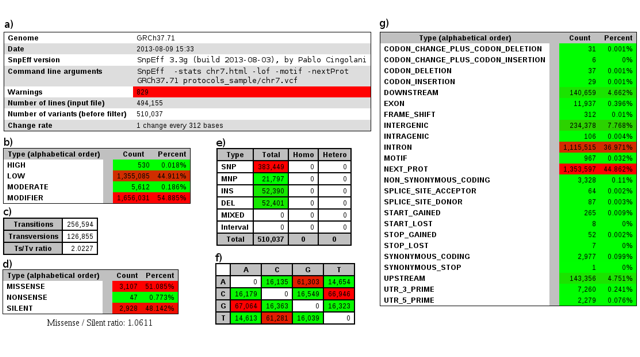
\includegraphics[width=14cm]{snpeff_1.png}
    \caption{Summary file produced by SpnEff. a) Overall summary showing input file, number of variants, command line, errors and warnings; b) number of impact assessed in each category; c) Transitions vs transversions; d) number of missense, nonsense and silent SNPs; e) number of variants by type (SNV, MNP, insertions, deletions and mixed); f) base change matrix; g) number of effects in each category.}
    \label{fig:snpeff1}
\end{figure}

\paragraph{Step 2. Counting variants in case and control subjects} In the first step of our protocol, SnpEff created a VCF file with half million annotated variants. Rather than scanning each annotation manually, we will use the SnpSift program to create a filter that will identify a small subset of variants with interesting functional properties. Since the VCF files used in most sequencing studies are even larger than the one in this example, our overall approach is to start by creating a filter using a very restrictive set of criteria. If no relevant variant is found using this stringent filter, we will relax the criteria to include variants with lower predicted impact.

In our example, since the pedigree is consistent with a Mendelian recessive disease, so we will first use SnpEff to find high impact variants that are homozygous in cases and either absent or heterozygous in controls. This provides a very strong genetic argument to select the promising variants and will be used as the first step in our filter. To do this, we will identify the case and control samples by providing SnpEff with pedigree information using a ``TFAM" file (a standard file format used to describe pedigrees). In our example, the TFAM file (\texttt{pedigree.tfam}) identifies the three cases (NA12879, NA12885, NA12886), and lists the other family members as controls. The \texttt{caseControl} command instructs the SnpSift program to count the number homozygous non-reference, heterozygous and allele count (number of non-reference alleles in each DNA sample) for both cases and controls groups (running time: $~60$ minutes):

\begin{lstlisting}[language=bash]
java -Xmx1g -jar SnpSift.jar \
       caseControl \
       -v -tfam protocols/pedigree.tfam protocols/ex1.eff.vcf \
       > protocols/ex1.eff.cc.vcf
\end{lstlisting}

This analysis creates an output VCF file (\texttt{ex1.eff.cc.vcf}) by adding new information to the \texttt{INFO} field for each variant: this includes information such as \texttt{Cases=1,1,3} and \texttt{Controls=8,6,22}, which correspond to the number of homozygous non-reference, heterozygous and total allele counts in cases and controls for each variant. The program also calculates basic statistics for each variant based on the allele frequencies in the two groups using different models, which can be useful as a starting point for more in-depth statistical analysis.

\paragraph{Step 3. Filtering variants} We can use the \texttt{SnpSift filter} command to reduce the number of candidate loci base on alleles in cases and controls. SnpSift \texttt{filter} allows users to create powerful filters that select variants using Boolean expressions containing data from the VCF fields. The expression we use to filter the VCF file \texttt{ex1.eff.vcf} is developed based on the expectation that all the three cases and none of the controls to be homozygous for the mutation. This is expressed using the following filter: \texttt{(Cases[0] = 3) \& (Controls[0] = 0)}. The full command line is:

\begin{lstlisting}[language=bash]
cat protocols/ex1.eff.cc.vcf \
    | java -jar SnpSift.jar filter \
         "(Cases[0] = 3) & (Controls[0] = 0)" \
    > protocols/ex1.filtered.hom.vcf
\end{lstlisting}

The filtered output file, \texttt{filtered.hom\_cases.vcf}, contains over 400 variants satisfying our criteria. This is still too large to analyze by hand, so can we can add another filter to see if any of these variants is expected to have a high impact. To identify variants where any of these impacts is classified as either \textit{HIGH} or \textit{MODERATE}, we add the condition \texttt{EFF[*].IMPACT = 'HIGH') | (EFF[*].IMPACT = 'MODERATE')}. The new filtering commands become:

\begin{lstlisting}[language=bash]
cat protocols/ex1.eff.cc.vcf \
    | java -jar SnpSift.jar filter \
            "(Cases[0] = 3) & (Controls[0] = 0) & ((EFF[*].IMPACT = 'HIGH') | (EFF[* ].IMPACT = 'MODERATE'))" \
    > protocols/ex1.filtered.vcf
\end{lstlisting}

After filtering, only two variants satisfy our criteria (Figure \ref{fig:snpefffilteredvars}), one of them is a \textit{STOP\_GAINED} loss of function variant, whereas the other one is a \textit{NON\_SYNONYMOUS} amino acid change. The first one is a known Cystic fibrosis variant.

\begin{figure}
    \centering
    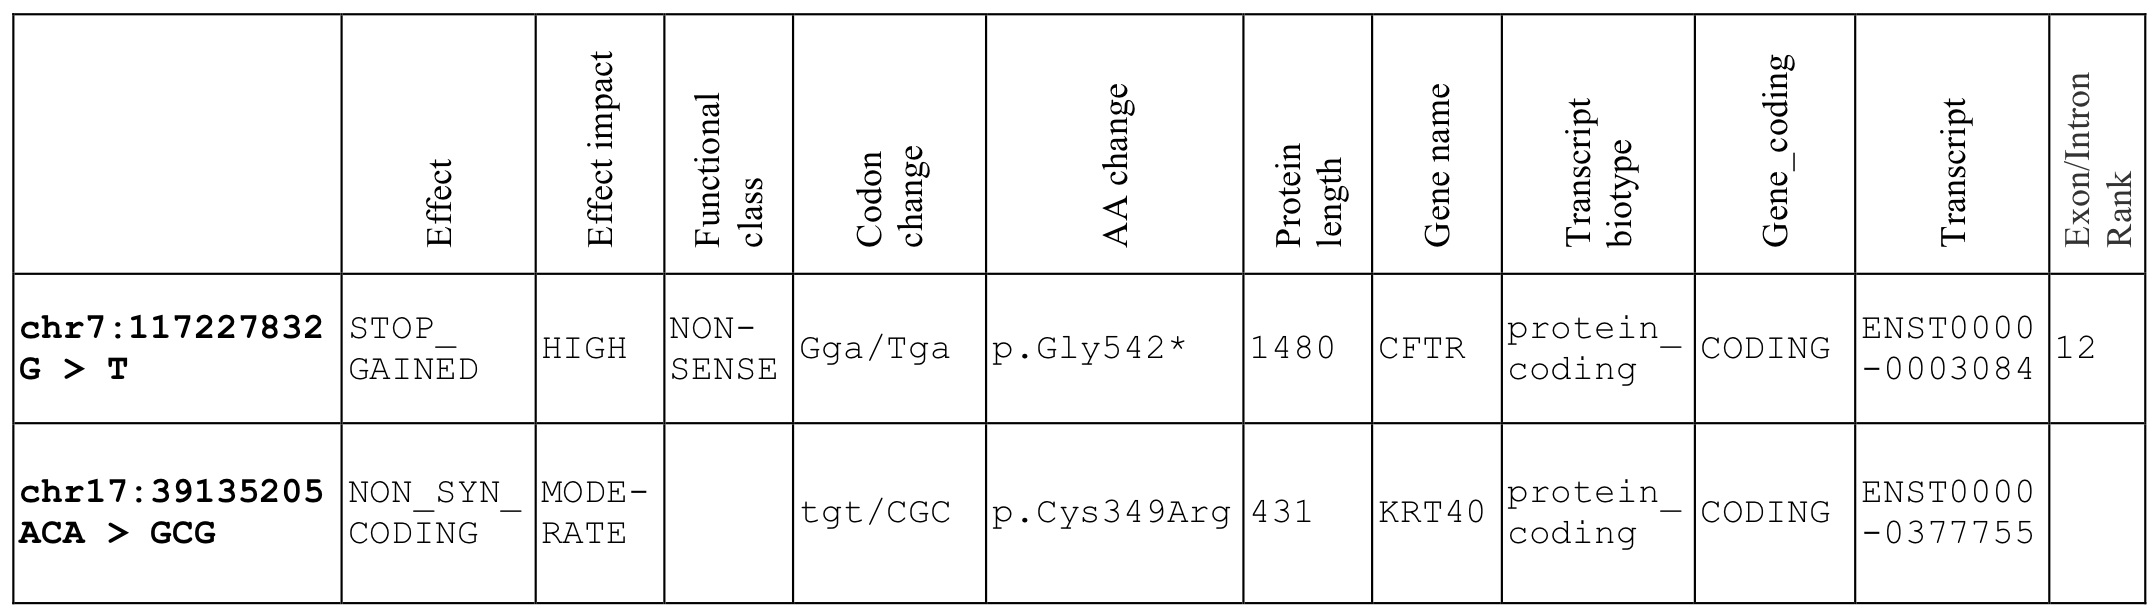
\includegraphics[width=14cm]{snpeff_table_variants_filtered.png}
    \caption{Candidate variants remaining after filtering.}
    \label{fig:snpefffilteredvars}
\end{figure}

A chart showing how the variant propagates across the pedigree structure (Figure \ref{fig:snpeff2}) can be created as follows:

\begin{lstlisting}[language=bash]
java -jar SnpSift.jar pedShow \
       protocols/pedigree.tfam protocols/ex1.filtered.vcf protocols/chart
\end{lstlisting}

\begin{figure}
    \centering
    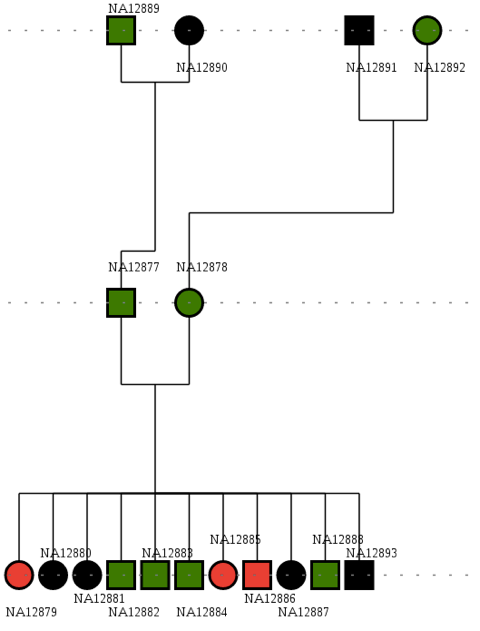
\includegraphics[width=8cm]{snpeff_2.png}
    \caption{Pedigree used for Procedure 1. A pedigree, created using the "SnpEff pedShow" command, shows heterozygous individuals in green, and homozygous alternative in red. It shows how the cystic fibrosis variant gets propagated from heterozygous unaffected grandparents and parents to homozygous affected offspring.}
    \label{fig:snpeff2}
\end{figure}

\paragraph{Step 4. Using clinical databases.} So far, since the purpose of the example was to show how annotations and filtering are performed to uncover new variants, we assumed that the causative variant was not known. In reality the variant is known and databases, such as ClinVar, have this information in convenient VCF format that can be used for annotations. We can annotate using ClinVar by using the following command:

\begin{lstlisting}[language=bash]
java -Xmx1g -jar SnpSift.jar annotate \
       -v protocols/db/clinvar_00-latest.vcf protocols/ex1.eff.cc.vcf \
       > protocols/ex1.eff.cc.clinvar.vcf
\end{lstlisting}

Our variant of interest is then annotated as \textit{``Cystic Fibrosis"} (to find the variant, we filter for variants having ClinVar annotation \textit{``CLNDBN"} that are in CFTR gene and have a \textit{STOP\_CODON} annotation):

\begin{lstlisting}[language=bash]
cat protocols/ex1.eff.cc.clinvar.vcf | java -jar SnpSift.jar filter \
     "(exists CLNDBN) & (EFF[*].EFFECT = 'STOP_GAINED') & (EFF[*].GENE = 'CF TR')"
\end{lstlisting}

\paragraph{Software Integration (Optional)} Sequence analysis software is often run in high performance computers combining several programs into processing pipelines. Annotations and impact assessment software needs to provide integration points with other analysis steps of the pipeline. In the following paragraphs we describe how to integrate SnpEff with two programs commonly used in sequencing analysis pipelines: i) Genome Analysis toolkit (GATK 2), a command-line driven software; and ii) Galaxy 3, a web based software.

\paragraph{GATK} The Genome Analysis Toolkit 2 is one of the most popular programs for bioinformatics pipelines. Annotations can be easily integrated into GATK using SnpEff and GATK’s VariantAnnotator module. Here we show how to annotate a file using SnpEff and GATK, as an alternative way of performing step 1. You should perform this step only if your processing pipeline is based on GATK: compared to running SnpEff from the command line, the results obtained when using GATK will only contain the highest impact annotation for each variant. This was a conscious trade-off made by the designers of GATK, partly because most biologists do this implicitly when reading a list of variants, but also to improve the readability and reduce the size of the annotation results.

The method requires two steps: i) Annotating a VCF file using SnpEff and ii) using GATK’s VariantAnnotator to incorporate those annotations into the final VCF file. When using SnpEff for GATK compatibility, we must use the \texttt{-o gatk} command line option:

\begin{lstlisting}[language=bash]
java -Xmx4g -jar snpEff.jar -v \
       -o gatk GRCh37.75 protocols/ex1.vcf \
       > protocols/ex1.eff.gatk.vcf
\end{lstlisting}

Next, we process these variants using GATK. For this step to work correctly, we need to make sure that our data files are compatible with the requirements GATK places on reference genomes (see GATK’s documentation for more details): (i) in the fasta file, chromosomes are expected to be sorted in karyotypic order; (ii) a genome fasta-index file must be available; and (iii) a dictionary file must be pre-computed. Assuming these requirements are satisfied, we can run the following command, which will produce a GATK annotated file (\texttt{ex1.gatk.vcf}):

\begin{lstlisting}[language=bash]
java -Xmx4g -jar $HOME/tools/gatk/GenomeAnalysisTK.jar \
       -T VariantAnnotator \
       -R $HOME/genomes/GRCh37.75.fa \
       -A SnpEff \
       --variant protocols/ex1.vcf \
       --snpEffFile protocols/ex1.eff.gatk.vcf \
       -L protocols/ex1.vcf \
       -o protocols/ex1.gatk.vcf
\end{lstlisting}

Note: We assumed GATK is installed in \texttt{\$HOME/tools/gatk/} and the reference genome is contained in \texttt{\$HOME/genomes/GRCh37.75.fa}. These file locations should be adapted to the actual path in your computer.

\paragraph{Galaxy} Another popular tool in bioinformatics is Galaxy 3, which allows pipelines to be created in a web environment using graphical interface, making it flexible and straightforward to use. SnpEff provides Galaxy modules (see http://snpeff.sourceforge.net/SnpEff\_manual.html\#galaxy for details). Once these modules are installed, we can run our sample annotation pipeline in Galaxy (Figure \ref{fig:snpeff3}). A step-by-step tutorial can be found at http://snpeff.sourceforge.net/protocol

\begin{figure}
    \centering
    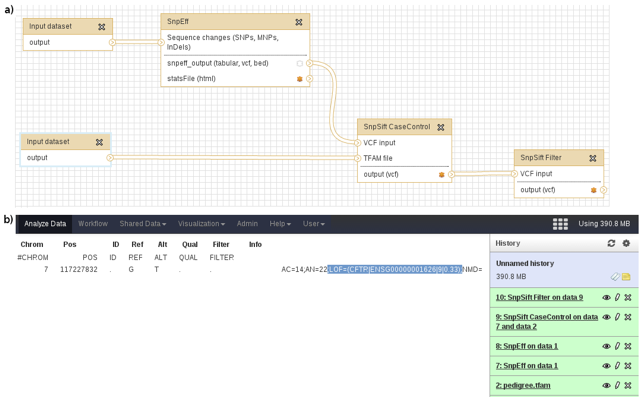
\includegraphics[width=14cm]{snpeff_3.png}
    \caption{Use of Galaxy combined with SnpEff. (a) Galaxy Protocol for example 1. Galaxy automatically creates a pipeline showing the processing steps, which can be modified and later used to process new datasets; (b) Results after the last step was executed by Galaxy server.}
    \label{fig:snpeff3}
\end{figure}

%---
\section{PROCEDURE II: Analysis of non-coding variants}
%---

This example shows how to perform basic annotation of non-coding variants. It is based on a short list of 20 non-coding that were identified by sequencing a 700 kb region surrounding the gene T-box transcription factor (TBX5) in 260 patients with congenital heart disease 67. TBX5 is a transcription factor that plays a well-established dosage-dependent role in heart and limb development. Coding mutations in TBX5 have been frequently identified in patients with Holt–Oram syndrome, which is associated with abnormal hand, forearm and cardiac development.

\paragraph{Step 1. Annotating variants} We will perform non-coding variant annotation using SnpEff following a similar approach to Procedure I. In this case, we construct a command line that instructs SnpEff to include motif information (\texttt{-motif}) and putative transcription factor binding sites (TFBS) identified in the ENSEMBL Regulatory Build and the Jaspar database:

\begin{lstlisting}[language=bash]
java -Xmx4g -jar snpEff.jar -v \
       -motif GRCh37.75 protocols/ex2.vcf \
       > protocols/ex2.eff.basic.vcf
\end{lstlisting}

\paragraph{Step 2. Adding custom regulatory information} A quick scan through the results shows that most variants are catalogued as \textit{INTERGENIC}, and none of them is associated with a known TFBS. This is not surprising since TFBS are small and also because regulatory elements involved in cardiac or limb development may not be widely active in commonly studied adult tissues. In this case, basic annotations did not provide additional information that can be used to narrow down the list of candidate SNVs. To solve this, the authors examined data from other sources, including ChIP-seq data for H3K4me1 (a post-translationally modified histone protein found in transcriptionally active genome regions, including enhancers and promoters). Data produced from ChIP-Seq analysis are frequently published in BED, BigBed or similar formats, which can be used directly by SnpEff by adding the ``-interval" command line option. This command line option can be used to add annotations using ChIP-Seq experiments from the ENCODE and Epigenome Roadmap projects: since multiple ``-interval" options are allowed in each command line, it is a simple way to combine several annotations:

\begin{lstlisting}[language=bash]
java -Xmx4g -jar snpEff.jar -v \
       -motif -interval protocols/ex2_regulatory.bed GRCh37.75 \
       protocols/ex2.vcf \
       > protocols/ex2.eff.vcf
\end{lstlisting}

In the output VCF file, variants intersecting genomic regions from the \texttt{-interval} command line option are annotated as \texttt{CUSTOM[ex2\_regulatory]} : the name in brackets identifies the file name provided to distinguish multiple annotation files.

\paragraph{Step 3. Adding conservation information} In order to refine our search, we can also look for variants in highly conserved non-coding bases. SnpEff natively supports PhastCons scores, but can also add annotations based on any other user-defined score provided as a Wig or VCF file. The command line for annotating using the PhastCons score is:

\begin{lstlisting}[language=bash]
java -Xmx1g -jar SnpSift.jar \
      phastCons -v protocols/phastcons protocols/ex2.eff.vcf \
      > protocols/ex2.eff.cons.vcf
\end{lstlisting}

Now we can filter our results looking for a highly conserved SNP in the regulatory region. We do this by using a \texttt{SnpSift filter} command and the appropriate Boolean expression:

\begin{lstlisting}[language=bash]
cat protocols/ex2.eff.cons.vcf \
    | java -jar SnpSift.jar filter \
            "(EFF[*].EFFECT = 'CUSTOM[ex2_regulatory]') & (exists PhastCons) & (PhastC ons > 0.9)" \
    > protocols/ex2.filtered.vcf
\end{lstlisting}

SnpSift \texttt{filter} supports a flexible syntax to create Boolean expressions using the annotation data that provides a versatile way to prioritize shorter lists of SNPs for subsequent validation. This syntax is described in detail in the online manual (http://snpeff.sourceforge.net/SnpSift.html\#filter). In this example, our filter results in only two candidate SNPs, one of which was extensively validated in the original study and is assumed to be causative 67.

The principles illustrated in our example for a small set of SNVs can be applied to millions of variants from whole genome sequencing experiments. Similarly, although we filtered the SNVs using \texttt{custom} ChIP-seq data that provided in the original study 67, regulatory information from public Encode or Epigenome Roadmap datasets could be used in a first line investigation before generating our own Chip- seq or RNA-seq data using disease-relevant cells and tissues.

\section{TROUBLESHOOTING}

Complete documentation for SnpEff, together with troubleshooting instructions are available at http://snpeff.sourceforge.net/SnpEff\_manual.html.

\section{ACKNOWLEDGEMENTS}

We thank Louis Létourneau and Adrian Platts, for their valuable suggestions for improving SnpEff. This work was funded by the National Institute of Diabetes \& Digestive \& Kidney diseases (NIDDK 5-U01- DK085545-02) and the Canadian Institutes for Health Research (CIHR MOP-102703).

	
%-----------------------------------------------------------------------------
\chapter{Epistatic GWAS analysis\label{ch:gwas}}
%-----------------------------------------------------------------------------

%---
\section{Preface}
%---


In recent years, over 80 genetic loci related to T2D have been identified \cite{morris2012large, consortium2014genome}. Nevertheless, the overall effect sizes of these loci account for less than 10\% of the overall disease predisposition \cite{manolio2009finding}. This poses the question of why, given that so much efforts has been directed at finding the genetic components of this disease, the loci found so far have such modest effects. This lack of large genetic effects, known as the ``missing heritability" problem, does not only arise in T2D but also in almost all complex traits. In recent studies about missing heritability \cite{zuk2012mystery, zuk2014searching} it was proposed that this effect might be partly explained by taking into account epistasis (i.e. gene interactions).

In this chapter, we propose a novel framework that takes into account putative epistatic interactions into genome wide association studies (GWAS). 

%We detect putative interactions by means of a co-evolutionary model that we develop based on Markov evolutionary theory. We fit the co-evolutionary model's parameters using protein structural data (PDB) an genome wide multiple sequence alignments (UCSC's 100-way). Once this model is parametrized, we perform genome wide association using of pairs of variants  from a sequencing study by incorporating the co-evolutionary model as priors in a Bayesian Framework.

Although this thesis focusses on the development of computational approaches that could be applied to the study of a number of complex diseases, our focus has been on type II diabetes mellitus (T2D), a complex disease first described by the Egyptians in 1500 BCE. Later the Greeks in 230 BCE used the term ``diabetes" meaning ``pass through" (or ``siphon") denoting the constant thirst and frequent urination of the patients. In the 1700s the term ``mellitus" (from honey) was added to denote that the urine was sweet and would ``attracts ants".

Diabetes symptoms include frequent urination, thirst, and constant hunger, high blood sugar (hyperglycemia) and insulin resistance. Long term complication from T2D may include eyesight problems, heart disease, strokes and kidney failure. Type II diabetes, is highly correlated with obesity and disease rate has increased dramatically during the last 50 years. According to the World Health Organisation the prevalence of diabetes is 9\% in adults and an estimated 1.5 millions deaths were caused by diabetes in 2012 \cite{guariguata2014global}, which is predicted to be the 7th leading cause of death by 2030. The costs associated to treating diabetes patients only in the U.S. are estimated around \$245 billion dollars.

The rest of the chapter is published in: \textbf{P. Cingolani}, R. Sladek, M. Blanchette, ``A co-evolutionary approach for detecting epistatic interactions in genome-wide association studies"

%---
\section{Abstract}
%---

\paragraph{Motivation} Epistasis, broadly defined as genetic interactions, is one of the likely causes why genome-wide association studies (GWAS) account for a small portion of heritable disease risk. Due to their high complexity, reduced statistical power and sometimes prohibitive computational requirements, epistatic GWAS have rarely been performed. 

\paragraph{Methods} In this paper, we propose a novel methodology for analysing putative epistatic interactions by combining multiple genome alignments and sequencing information. Using protein structures for individual and co-crystallized complexes information and genome wide multiple species alignment we create a co-evolutionary model that allows the calculation of the posterior probability of physical interaction between residues given evolutionary data. These probabilities are then used as the interaction priors for an epistatic GWAS analysis as basis for genome wide Bayesian framework. 

\paragraph{Results} Our optimized algorithms can be applied to genome wide scale sequencing studies for tens of thousands of samples, that typically yield millions of variants. We applied our approach to a large type II diabetes (T2D) case-control cohort and inferred a number of putative interactions associated with increased risk of developing T2D. 

\paragraph{Availability} Our code is publicly available at \texttt{github.com/pcingola/Epistasis}

%---
\section{Introduction}
%---

Genetic studies aim to discover how a phenotype of interest, such as disease risk or height, is affected by in individual's genetic background. Genome wide association studies (GWAS) are powerful techniques aimed at finding statistical associations between a phenotype and genetic variants \cite{clarke2011basic}. Although several genetic variants related to different phenotypes have been found, variants discovered in GWAS so far can only explain a small part for the phenotypic heritability. For instance, all genetic variants associated to height collectively account for few centimetres in the offspring's height \cite{wood2014defining}. Similarly the known variants related to type 2 diabetes risk collectively explain only 5\% to 10\% of the overall variance in disease predisposition \cite{morris2012large, consortium2014genome}. This problem is known as ``missing heritability" \cite{manolio2009finding} and recent theories suggest that genetic interactions (epistasis) might play an important role in it \cite{zuk2012mystery, zuk2014searching}.

The foundations for epistasis \cite{gao2010classification}, have been proposed almost a hundred years ago by Bateson (1909) and Fisher (1918). It was the latter who coined the term to denote a ``statistical deviation of multilocus genotype values from an additive linear model for the value of a phenotype" \cite{gao2010classification}. There is evidence of such interactions being involved in complex diseases. For instance an interaction between BACE1 and APOE4 having a significant association with Alzheimer's disease has consistently been replicated in different studies \cite{combarros2009epistasis}. Many types of situations can lead to epistatic interactions. Among them, perhaps the most common involved pairs of variants that encode amino acids whose physical interactions is regulated for their function.

One of the main problems in finding association between interactions and disease is that out of the whole set of molecular interactions (the interactome) only a small part of it has been characterized \cite{venkatesan2009empirical}. Interacting proteins can be identified experimentally through several types of approaches (yeast two hybrid, protein fragment complementation assay, glutathione-s-transferase, affinity purification coupled to mass spectrometry, tandem affinity purification, etc. \cite{shoemaker2007deciphering}) and large databases of protein-protein interactions are now available for human \cite{stark2006biogrid, shoemaker2007deciphering}. In almost all cases, these methods identify the presence of an interaction between proteins but do not discern the exact residues mediating such interactions. Furthermore, it is estimated that up to 80\% of the human protein-protein interactions remains unknown \cite{venkatesan2009empirical}.

These issues can be partially addressed using computational predictions of either pairs of interacting proteins or interacting residues \cite{shoemaker2007decipheringP2}. A type of approaches that has been gaining popularity recently is one that makes use of the plethora of genomic sequences available for species other than human in order to discover evolutionary evidence of selective pressure on pairs of residues to identify interacting sites and interfaces \cite{marks2012protein}. Interacting residues and their neighbours may then be subject to compensating epistasis, where a mutation at a residue in one protein may be compensated by another mutation at a residue in the second protein \cite{pazos1997correlated}.For example assuming that evolutionary pressure acts on both interaction sites simultaneously, co-occurring compensatory mutations can become fixed in the population with higher probability than non-compensatory ones. In light of this hypothesis, one can use statistical methods on multiple sequence alignments of proteins from different organisms to find coevolving sites. This types of approaches has been used to identify coevolving sites both within a protein (e.g. N-terminal and C-terminal domains in PKG protein \cite{goh2000co}, GroES-L chaperoning system \cite{ruiz2013coevolution}, $\alpha$ and $\beta$ haemoglobin subunits \cite{pazos1997correlated}), and between interacting proteins (e.g. G-protein coupled receptors and protein ligands \cite{goh2000co}).

Many methods exist to find putative interaction loci, both within and across proteins, based on evolutionary evidence (see \cite{de2013emerging} for a review). One of the simplest methods for inferring co-evolution uses mutual information between two loci \cite{marks2012protein} in a multiple sequence alignment. However, methods based on correlation or mutual information are known to have systematic biases due to the fact that they ignore phylogenetic relationships \cite{de2013emerging}, or sequence heterogeneity problems \cite{weigt2009identification}. More sophisticated methods, such as DCA \cite{morcos2011direct}, PSICOV \cite{jones2012psicov} or mdMI \cite{clark2014multidimensional} try to overcome these biases, however they are usually not suitable for GWAS-scale analysis for two main reasons. First, they require multiple alignments of a very large number of sequences (ranging from $400$ to $25L$, where $L$ is the length of the protein \cite{clark2014multidimensional}), and such depth is not usually available at whole genome scale. Second, they are computationally demanding (e.g. running for minutes or even days for each interacting pair of proteins being considered), making them unsuitable for analyses involving millions of variants spanning over thousands of proteins. Furthermore, a recent study shows that overall agreement between methods is not high (65\% or less) and predictive power is quite low (only 6\% of the ``top scoring pairs" are real interactions) \cite{clark2014multidimensional}.

Applying epistatic interaction models to GWAS studies is a challenging problem for several reasons: i) interaction models are by definition non-linear \cite{gao2010classification}; ii) analyzing all order $N$ variant combinations requires great computational power and efficient algorithms because the number tests grows exponentially with $N$ \cite{phillips2008epistasis}; iii) multiple hypothesis testing correction can render association tests underpowered for all but very large cohorts \cite{gao2010classification, phillips2008epistasis}; and iv) there is no consensus of what genetic interaction means, which is reflected in the difficulty to find a unified model \cite{phillips2008epistasis,mani2008defining}. For all these reasons and due to the lack of sequencing cohorts large enough to detect these interactions, the application of epistatic models to sequencing studies has not been widespread. Furthermore, there is no clear consensus on the required sample size to detect epistatic interactions. Depending on phenotypic effect size and variant's allele frequency some estimates assume in the order of 10,000 to 500,000 cases \cite{jostins2013using} to be required. Such cohorts are now becoming feasible due to improvements and cost reductions in sequencing technology.

Approaches for epistatic GWAS do exist and they apply a wide array of methodologies. In \cite{zhao2006test}, the authors infer epistatic probabilities by noting that interactions create linkage disequilibrium patterns in the disease population. A Bayesian framework is applied in \cite{zhang2007bayesian} taking into account several risk models, using Dirichlet priors the distribution for each model can be solved analytically, then the combined model's posterior distribution is calculated using an MCMC sampling technique. In \cite{ackermann2012systematic}, the authors look for over / under-represented allele pairs in a given population by performing an analysis of imbalanced allele pair frequencies. Finally, finding interacting variants can be viewed as an attribute selection problem, thus many machine learning methodologies have been proposed \cite{mckinney2006machine}. While all algorithms have relative advantages, there is no standard in epistatic analysis, we believe that we can create better methods by combining other sources of biological information, such as evolutionary evidence.

In this work we propose an approach to prioritize pairs of variants identified in case/control cohorts by combining genome wide association with epistatic interaction models. In a nutshell, our method uses recently computed 100-way vertebrate genome alignments \cite{blanchette2004aligning} to calculate interaction posterior probabilities for any given pair of residues in human proteins. This is achieved by contrasting the likelihood of the observed pair of alignment columns under a joint substitution model that factors in dependencies between interacting sites, and a null model of independent evolution.  These posterior probabilities are then used as priors to modulate the evidence of epistatic interaction derived from GWAS data. Our implementation is sufficiently efficient to be applied to GWAS-scale datasets of tens of thousands of samples. Finally we apply this methods to a cohort of $\sim 13,000$ individuals in a case-control study of type II diabetes (for study details, see \cite{mccarthy2015T2D}) and identify suggestive associations of putatively epistatic interactions.

%---
\section{Methods \label{sec:gwasMeth}}
%---

Our epistatic GWAS analysis pipeline involves three key steps, as shown in Figure \ref{fig:gwaspipeline}. First, we learn a co-evolutionary substitution rate matrix for pairs of amino acids that are in contact in proteins. Second, we analyze a GWAS data set to identify pairs of non-synonymous SNPs that show (possibly weak) evidence of epistasis. Third, for each pair of SNP identified in step 2, we measure the evidence of co-evolution of the pair of encoded amino acids, and combine it with the GWAS evidence by adding up the corresponding Bayes factors.

\fig{gwas_epistasis_pipeline}{gwaspipeline}{14cm}{Complete pipeline example}{Complete pipeline example}

\subsection{Substitution model for pairs of interacting amino acids \label{sec:gwasQ2}}

In this section, we describe how we estimate two substitution rate matrices. The first is the usual $20 \times 20$ substitution rate matrix $Q$ describing the evolution of individual amino acids. The second, $Q_2$, is a $400 \times 400$ substitution rate matrix for pairs of interacting residues. 

We used the 100-way vertebrate multiple sequence alignment and accompanying phylogenetic tree $T$ available from the UCSC Genome Browser \cite{karolchik2014ucsc}. This alignment includes the DNA sequences of 100 species whose genome is completely or nearly completely sequenced, with 12 primates, 44 non-primates eutherians, 5 marsupials, 14 birds, 6 reptiles, 16 ray-finned fish and 8 lobe-fined fish.
%6 Afrotheria, 14 Avians, 14 Euarchontoglires, 16 Fish, 25 Laurasiatheria, 5 Mammalians, 12 Primates and 8 Sarcopterygii. 
The multiple alignment is performed using ``multiz" algorithm \cite{blanchette2004aligning,kielbasa2011adaptive}.

From the $\sim 21,000$ human protein structures (resolution less than $3$ \r{A}) available in Protein Data Bank, we extracted a set of $\sim770,000$ pairs of ``within protein interactions" residues, defined as pairs of residues from the same protein where at least one pair of atoms is within $3$ \r{A}  or less. Similarly, from the set of $\sim5,700$ models of co-crystallized complexes in PDB, we extracted a set of $\sim12,000$ pairs of ``protein-protein interacting" residues, defined as amino acids from different proteins that satisfy the same distance criterion.

To derive rate matrix $Q$, we consider the complete set of $n \sim 22 \times 10^6$ protein coding sites present in the alignment, irrespective of the presence or absence of contacts. $Q$ is obtained following classical sequence evolution theory (\cite{yang2006computational, felsenstein2004inferring}). First, for each pair of species  $s_i$ and $s_j$, we obtain $c_i(a)$ defined as the count of amino acid $a$ in species $s_i$, and $c_{i,j}(a,b)$ defined as the number of sites that have had a transition from amino acid $a$ in $s_i$ to $b$ in $s_j$. Stationary probability of amino acid $a$ in genome $s_i$ is then defined as $\pi_i = c_i(a)/n$. Assuming a time reversible model, we get the frequency of change from $a$ to $b$: $f_{i,j}(a,b) = f_{j,i}(a,b) = (c_{i,j}(a,b) + c_{j,i}(a,b))/(2n)$. Let $P_{i,j}$ be the amino acid transition probability matrix from $s_i$ to $s_j$, i.e. $P_{i,j}(a,b)$ is the probability that species $s_j$ has amino acid $b$ given that species $s_i$ has amino acid $a$. Then $P_{i,j}$ is obtained through the relation $f_{i,j}(a,b) = \pi_i(a) \cdot P_{i,j}(a,b)$, or $P_{i,j}(a,b) =   f_{i,j}(a,b) /  \pi_i(a)$.  Let $t_{i,j}$ be the total branch length between $s_i$ and $s_j$ (obtained from the phylogenetic tree). Assuming time reversibility, we have $P_{i,j} = e^{Q \cdot t_{i,j}}$, and thus $Q=log[ P_{i,j} / t_{i,j} ]$ \cite{yang2006computational}. Taking into account the estimation error, the equation becomes $\hat{Q}(t_i+t_j) = Q = log[ P_{i,j} / t_{i,j} ] + \epsilon_{i,j}$, where $\epsilon_{i,j}$ is an error matrix. Under the assumption that the mean error is zero, we can approximate the rate matrix by the calculating an average of all estimates:

\begin{eqnarray*}
	\hat{Q} & = & \frac{1}{N(N-1)/2} \sum_{i < j} \hat{Q}_(t_i+t_j) \\
	            & =  & \frac{2}{N(N-1)} \sum_{i<j} \frac{1}{t_i+t_j} log[ \hat{P}_(t_i+t_j) ]
\end{eqnarray*}

The much larger substitution matrix $Q_2$ describes the substitution rate from any pair of amino acids $(a,b)$ to any other pair $(c,d)$. It is derived similarly to $Q$, but considering only pairs of amino acids from the set of within protein interacting pairs of amino acids. We only take into account amino acids pairs within the same chain, that are separated by 20 amino acids or more. 

\subsection{Calculating likelihood of individual and pairs of alignment columns}

Given a substitution rate matrix $Q$, the likelihood $L_1[MSA(i)]$ of an alignment column $MSA(i)$ assigning an amino acid to each leaf in the tree $T$ is calculated using the well known Felsenstein algorithm \cite{felsenstein2004inferring}. This is achieved in time $O(N \cdot |\Sigma|^2)$, where $|\Sigma|=20$ and $N$ is the number of sequences in the alignment. Given matrix $Q_2$, the same algorithm can be used to compute the likelihood $L_2[ MSA(i), MSA(j) ]$ of a pair of alignment columns $( MSA(i), MSA(j) )$, but now in time $O(N \cdot |\Sigma|^4)$. 

A test for co-evolution of two positions $i$, $j$ of the same or different proteins is obtained using the likelihood ratio under the two models: 

\begin{eqnarray*}
	L_C[MSA(i), MSA(j)] = \frac{L_2[ MSA(i), MSA(j) ]}{L_1[MSA(i)] \cdot L_1[MSA(j)]}
\end{eqnarray*}

\noindent where the denominator assumes that the amino acids $i$ and $j$ evolve independently. Similarly, the log-likelihood is defined as

\begin{eqnarray}
    \ell_C[MSA(i), MSA(j)] = log \left[ \frac{L_2[ MSA(i), MSA(j) ]}{L_1[MSA(i)] \cdot L_1[MSA(j)]} \right]
\end{eqnarray}
%	LL[M_{SA}(i,j)] = log \left[ \frac{P(i, j | M_{SA}, Q_2)}{P(a_i | M_{SA}, Q) \cdot P(a_j | M_{SA}, Q)} \right]dd
%Given a pair of columns in the multiple sequence alignment $M_{sa}$, the corresponding phylegentic tree $\mathcal{T}$, we calculate the likelihood ratio by propagating the probabilities from the leaves up the root of the phylogenetic tree using Felsestein's algorithm \cite{felsenstein2004inferring} using transition matrices $Q$ and $Q_2$ for the null and alternative models respectively.

Because the calculations described in this section will need to be performed on a very large number of pairs of sites, optimizations we are required to ensure manageable running time. First, pre-calculation of  matrix exponentials $P(t) = e^{Qt}$ is necessary for all values of $t$ corresponding to individual branch lengths. Another optimization (``constant-tree caching") is used to cache likelihood values for subtrees of the phylogenetic tree where all nodes have the same amino acid values. This optimization results in speed-up only if the phylogenetic tree remains constant throughout the genome, which is the case in our model.

\subsection{GWAS model}

Consider a GWAS with $N_S$  samples (individuals) and $N_V$ variants, we use the standard notation for phenotypes and code them as $d_s=1$ when individual $s$ is affected by disease and $d_s=0$ if it is "healthy". Let $\bar{d} = [d_1, ..., d_{N_s}]$ be a phenotype vector and $g_{s,i} \in \{0,1,2\}$ a genomic variant for sample $s$ at locus $i$. A logistic model of disease risk \cite{balding2006tutorial} is

\begin{eqnarray*}
    p_{s,i} & = & P( d_s=1 | g_{s,i}, \bar{\theta} ) \\
    & = & \phi( \theta_0 + \theta_1 g_{s,i} + \theta_2 c_{s,1} + \theta_4 c_{s,2} + ... ) \\
    & = & \frac{1}{1 + e^{\theta_0 + \theta_1 g_{s,i} + \theta_2 c_{s,1} + \theta_4 c_{s,2} + ...}} \\
    & = & \phi( \bar{\theta}^T \bar{g}_{s,i})
\end{eqnarray*}

\noindent where $\phi(\cdot)$ is the sigmoid function, $c_{s,1}, c_{s,2}, ... $ are covariates for each individual $s$ (these covariates usually include sex, age and eigenvalues from population structure analysis \cite{price2006principal}), $\bar{g}_{s,i} = [ 1, g_{s,i} , c_{s,1}, c_{s,2}, ... , c_{s,N_C} ]$, and $\bar{\theta} = [\theta_1, \theta_2, ..., \theta_m] $. The parameter estimates $\bar{\theta}$ are obtained by solving the maximum likelihood equation

\begin{eqnarray*}
    L( \bar{\theta} ) & = & \prod_{s=1}^{N_S}{ P( d_s | \bar{\theta}, g_{s,i} ) } \\
    & = & \prod_{s=1}^{N_S}{ p_{s,i}^{d_s} (1-p_{s,i})^{1-d_s} } \\
    & = & \prod_{s=1}^{N_S}{ \phi( \bar{\theta}^T \bar{g}_{s,i})^{d_s} (1-\phi( \bar{\theta}^T \bar{g}_{s,i}))^{1-d_s} }
\end{eqnarray*}

% where $p_{s,i} = P( d_s | \bar{\theta}, g_{s,i} )$ is the probability of individual $s$ disease outcome, given a genomic variant.

Using this model, we have two hypotheses: i) the null hypothesis, $H_0$, assumes that genotype does not influence disease probability (i.e. $\theta_1 = 0$). ii) the alternate hypothesis, $H_1$, assumes that the genotype does influence disease probability (i.e. $\theta_1 \neq 0$). We can compare these two hypotheses using a likelihood ratio test. We define

\begin{eqnarray} \label{eq:gwasLogLikLogReg}
	L_G & = & \frac{L( \bar{\theta} | H_1 ) }{ L( \bar{\theta}' | H_0 ) }\\
	\ell_G & = & log \left[ L_G \right] = log \left[ \frac{L( \bar{\theta} | H_1 ) }{ L( \bar{\theta}' | H_0 ) } \right]
\end{eqnarray}

\noindent where $\bar{\theta}'$ and $\bar{\theta}$ are the maximum likelihood estimates for null and alternate model respectively. According to Wilk's theorem \cite{wilks1938large}, the log likelihood ratio has a $\chi^2_1$ distribution under the null hypothesis, so we can easily calculate a p-value.

Next, we extend the logistic model to accommodate interacting loci. For an individual (sample $s$), we model interactions between two genetic loci $i$ and $j$, having genotypes $g_{s,i}$ and $g_{s,j}$, by extending the logistic model

\begin{eqnarray} \label{eq:gwasLogRegH1}
    P( d_s | g_{s,i},g_{s,j}, H_1) & = & \phi[ \theta_0 + \theta_1 g_{s,i} + \theta_2 g_{s,j} + \theta_3 (g_{s,i} g_{s,j}) \\
    & & ... + \theta_4 c_{s,1} + ... + \theta_m c_{s,N_{cov}} ] \\
    & = & \phi( \bar{\theta}^T \bar{g}_{s,i,j}) )
\end{eqnarray}

\noindent where $\bar{g}_{s,i,j} =  [1, g_{s,i}, g_{s,j}, ( g_{s,i} g_{s,j}), c_{s,1}, c_{s,2}, ..., c_{s,N_{cov}} ]^T$. An implicit assumption in this equation is that $g_{s,i}$ and $g_{s,j}$ are not correlated (e.g. they are not located in the same LD-Block). This can be enforced either by using haplotype structure information (e.g. from HapMap) or by limiting the application of the model to variants either in different chromosomes or sufficiently distant (say $> 1Mb$). The null hypothesis $H_0$ assumes that variants act independently

\begin{eqnarray} \label{eq:gwasLogRegH0}
    P( d_s | g_{s,i},g_{s,j}, H_0) & = & \phi[ \theta_0' + \theta_1' g_{s,i} + \theta_2' g_{s,j} + \theta_3' c_{s,1} + ... ] \\
   & = & \phi( \bar{\theta'}^T \bar{g}_{s,i,j}' )
\end{eqnarray}

\noindent where $\bar{g}_{s,i,j}' =  [1, g_{s,i}, g_{s,j}, c_{s,1} , c_{s,2}, ..., c_{s,N_{cov}} ]^T$.

We investigated several algorithms for logistic regression parameter fitting. The fastest convergence is obtained using Iterative Reweighted Least Squares (IRWLS \cite{daubechies2010iteratively}) and Broyden-Fletcher-Goldfarb-Shanno algorithm (BFGS \cite{broyden1970convergence}) with some code optimizations. In most cases, IRWLS converges faster, so it was selected as the default implementation in our analysis.

Another way to compare the null hypothesis to the alternative hypothesis, is using a Bayesian formulation \cite{kass1995bayes, wakefield2009bayes}

\begin{eqnarray*}
	P(H_1 | \mathcal{D}) & = & \frac{ P( \mathcal{D} | H_1) P(H_1) }{ P(\mathcal{D}) } = \frac{ \int{ P(\mathcal{D} | \bar{\theta} , H_1) P( \bar{\theta} | H_1) P(H_1)  d\bar{\theta} } }{ P(\mathcal{D}) }  \\
	\Rightarrow  \frac{ P(H_1 | D)  }{ P(H_0 | D)  } & = & \frac{ \int{ P(\mathcal{D} | \bar{\theta} , H_1) P( \bar{\theta} | H_1)  d\bar{\theta} } }{\int{ P(\mathcal{D} | \bar{\theta'} , H_0 ) P( \bar{\theta'} | H_0)  d\bar{\theta'} } } \frac{ P(H_1) }{ P(H_0)  }  
	=  B_F \frac{ P(H_1) }{ P(H_0)  }
\end{eqnarray*}

\noindent where $B_F$, the ratio of the two integrals, is the Bayes factor. Using a Bayesian formulation has two main advantages: i) the hypothesis are automatically corrected for model complexity since Bayes factor asymptotically converge to Bayesian Information Criteria (BIC) \cite{kass1995bayes}, and ii) we can compare non-nested models. The Bayes factor for the epistatic model becomes:

\begin{eqnarray}\label{eq:bf2}
	B_F = \frac
	{ \int{ \prod_{s=1}^{N_S}{ \phi( \bar{\theta}^T \bar{g}_{s,i,j})^{d_s} [ 1-\phi( \bar{\theta}^T \bar{g}_{s,i,j}) ]^{1-d_s} } P( \bar{\theta} | H_1)  d\bar{\theta} } }
	{ \int{ \prod_{s=1}^{N_S}{ 
	\phi( \bar{\theta'}^T \bar{g'}_{s,i,j} ) )^{d_s} 
	[ 1-\phi( \bar{\theta'}^T \bar{g'}_{s,i,j}) ]^{1-d_s} } 
	P( \bar{\theta'} | H_0)  
	d\bar{\theta'} } }
\end{eqnarray}

Calculating Bayes factors is challenging and most of the times there are no closed form equations. Calculating the integrals using numerical algorithms is possible, but  imposes a significant computational burden thus making it impractical for large datasets, such as GWAS data, even using large computing clusters. We can approximate the integrals using Laplace's method  \cite{kass1995bayes}. If $g(x)$ has a maximum at $x_0$, it can be shown that

\begin{eqnarray*}
	\int{e^{-\lambda g(x)} h(x) dx} & \simeq & h(x_0) e^{\lambda g(x_0)} \sqrt{\frac{2 \pi}{\lambda g''(x_0)}} \\
\end{eqnarray*}

The multivariate case, for $\bar{x} \in \Re^d$, is analogous: we just need a Hessian matrix instead of a second derivate of $g(\cdot)$

\begin{eqnarray}\label{eq:laplace}
	\int{e^{\lambda g(\bar{x})} h(\bar{x}) d\bar{x}} & \simeq & h(\bar{x}_0) e^{\lambda g(\bar{x}_0)} 
	\left( \frac{2 \pi}{\lambda} \right)^{d/2} \left[ \frac{\partial^2 g(\bar{x}) }{\partial \bar{x} \partial \bar{x}^T} \right] ^{-1/2}
\end{eqnarray}

Using equation \ref{eq:laplace} we can try to approximate the complex integrals in equation \ref{eq:bf2} by the transformation $L(\bar{\theta}) = e^{\ell(\bar{\theta})}$, where $\ell(\cdot)$ is the log-likelihood of the data. So, we can use Laplace approximation by using Eq.\ref{eq:laplace}, at the point of the maximum likelihood. In order to do so, we need to calculate the Hessian matrix in Eq.\ref{eq:laplace}. Fortunately, for logistic models, we can make a few simplifications. Considering that $L(\bar{\theta}) = \prod_{s=1}^{N_S}{ \phi( \bar{\theta}^T \bar{g}_s)^{d_s} [ 1-\phi( \bar{\theta}^T \bar{g}_s) ]^{1-d_i} }$, it can be shown that for genotype terms

\begin{eqnarray*}
	\frac{ \partial^2 \ell(\bar{\theta}) }{ \partial\theta_i \partial\theta_j } 
	= \sum_s{ g_{s,i} g_{s,j} p_s (1-p_s) } 
\end{eqnarray*}

Using analogous derivation for the covariates, we can find an analytic form of the Hessian, which completes the Laplace approximation formula.

Calculating Bayes factors involves using prior parameter distributions. In order to estimate these distributions, we run the logistic regression fitting analysis and plot the parameter distributions for different levels of significance. As expected most parameters have unimodal distribution, except for $\theta_3$, which has a multimodal distribution (Figure \ref{S3}). For all parameters, except $\theta_3$, we use a normal distribution centred at the mean and variance set to one ($\sigma=1)$ even though most times the variance is much smaller. This is done to avoid penalizing outliers too heavily and to have smooth derivatives near the maximum likelihood estimates. For $\theta_3$, which has a multimodal distribution, we fit a mixture model parameters using an EM algorithm, as shown in Supplementary Figure / Table \ref{S3??}.


\paragraph{Computational and statistical issues} It is easy to see that the computational burden for the detection of pairs of interacting genetic loci affecting disease risk is significantly larger than in a standard (single variant) GWAS study. A priori all pairs of variants should be analyzed, thus significantly increasing the number of statistical tests. This also reduces the statistical power since the required p-value significance level would be orders of magnitude smaller. A na\:ive approach would estimate that if a typical genetic sequencing study has $10^6$ variants, a GWAS on epistatic variants would square that number of statistical tests, thus p-values required for significance would be in the order of $0.05 / (10^6)^2 = 5 \cdot 10^{-14}$. 

Fortunately these numbers can be reduced significantly. First, in this study, we only concentrate on non-synonymous coding variants. Second, as required by our co-evolutionary model, only variants overlapping a multiple sequence alignment are taken into account (when several multiple sequence alignments overlapped a region, the alignment with the longest number of proteins was selected).Third, if two variants $g_i$ and $g_j$ are such that the interaction term $(g_{s,i} g_{s,j})$ is zero in all samples, which usually happens for pairs of rare variants, then $B_F = 1$. Fourth, if the variants and the epistatic term $[g_{s,i}, g_{s,j}, g_{s,i} g_{s,j}]$ are linearly dependent, the logistic regression result will be meaningless, so we can safely skip such variant pairs. Fourth, if one of the variants has high allele frequency respect to the other, all non-zero epistatic terms may lie in the same positions as non-zero genotypes from the low frequency variant, causing logistic regression estimates to artificially inflate the coefficients of the low frequency variant and the epistatic term thus creating an artificially high association (low p-value). So we filter out these variant pairs as well. Finally, we filter out all variants having Hardy-Weinberg p-value of less than $10^{-6}$, since these variants also artificially inflate the logistic regression coefficients.  Once the results are obtained, we can focus on interactions by further filtering results and keeping variant pairs whose alternative logistic model (see equation \ref{eq:gwasLogRegH1}) has small absolute values for $\theta_1$ and $\theta_2$ while having large absolute values for $\theta_3$, specifically we keep results if $|\theta_3| > K ( |\theta_1| + |\theta_2| )$ (based on empirical data, we set $K=3$). 

\subsection{Putting it all together}

In summary, we first calculate the transitions matrices for the Markov models ($Q$ and $Q_2$) based on observations from protein structures (PDB) and multiple sequence alignments (UCSC's 100-way). We analyze variants from genome sequencing data first by filtering only for non-synonymous variants, then analyzing all possible pairs of variants and filtering out those that are unsuitable for further analysis (e.g. in linear dependence, deviation from Hardy-Weinberg equilibrium having p-value less than $10^{-6}$, etc.). From the pairs of variants that pass filtering, we fit two logistic regression models (null and alternative hypothesis), then calculate a p-value using the log-likelihood ratio, and keeping pairs of variants having p-values below a predefined threshold ($10^{-6}$). These pairs of variants are then analyzed under our co-evolutionary model, we find the corresponding columns in the multiple sequence alignment and calculate the likelihoods for the null and alternative models by means of Felsenstein's algorithm (using matrices $Q$ and $Q_2$ in respectively). Finally, likelihoods from co-evolutionary model and likelihoods from logistic regression models are incorporated into a Bayes Factor equation, which is calculated using Laplace's approximation.

%---
\section{Results}
%---

Our approach, which is summarized in Figure ??, involves three main components. First we estimate evolutionary substitution rates for individual amino acids in a protein as well as for pairs of amino acids (either from the same protein or not) that are physically interacting. Given a set of multiple sequence alignment of protein sequences, these evolutionary models can be used to calculate the likelihood of interaction between any two given amino acids, without the need for any structural information. Second, a statistical test for epistasis is developed to identify pairs of non-synonymous SNPs that show (often weak) evidence of interaction in the way they associate to a given trait. Finally, information from the co-evolution component is combined with that from the epistasis component to give more power to the epistasis test.
 
\subsection{Co-evolutionary substitution models}

The approach described in Methods was used to obtain substitution rate matrix $Q$ for individual amino acids and $Q_2$ for pairs of physically interacting residues within the same protein. Unsurprisingly, $Q$ (or more precisely a transition matrix $P(t)$ obtained from $Q$) is very similar to well known transitions matrixes such as PAM \cite{} (Supplementary Figure \ref{f:S1} and Table \ref{tab:S1}).

%Estimating $Q_2$ requires information about amino acids that are known to be ``interacting". A pair of amino acids is considered to be ``interacting" if any pair of atoms (one from each amino acid) has a distance of $3$ \r{A} or less \cite{burger2010disentangling}. 

The structure of $Q_2$, which describes substitution rates between one pair of interacting amino acids to another, is richer (Supplementary Figure \ref{fig:S2} and supplementary file \ref{fileQ2_hat.txt}). Of particular interest are the pairs of pairs of amino acids for which the ratio $R(ab,cd) = Q_2 (ab, cd) / ( Q(a,c) \cdot Q(b,d) )$ is large. Those substitution pairs are the ones that are most strongly indicative of an interaction. Figure \ref{fig:q_q2_compare} shows that the number of pairs for which $R$ deviates significantly from 1 is quite large, arguing that interacting sites have co-evolutionary rates that differ from the bulk of non-interacting sites.

For example, the case with the highest rate ratio is \texttt{[V.I -> W.W]}' (i.e. amino acid 'V' switched to 'W' in the one sequence, and amino acid 'I' changed to 'W' in the other). In fact, the top 10 pairs are all transitions to 'W-W' amino acid pairs. This makes sense considering that (i) individual amino acid substitution rates to tryptophan are generally very low, but that (ii) tryptophan pairs are well known $\beta$-hairpin stabilizers and are considered as a paradigm for designing stable $\beta$-hairpins \cite{santiveri2010tryptophan}.

Another type of pair transitions with large ratio is the double transitions to a pair of phenylalanine amino acids from a pairs of hydrophobic amino acids (Lysine, Asparagine, Glutamine, Arginine, Aspartic acid and Glutamic acid). Phenylalanine-Phenylalanine interaction pairs are assumed to conform $\pi-\pi$ interactions which are predicted and experimentally observed to be energetically favourable \cite{hunter1991pi}.

\subsection{Co-evolutionary model validation}

We first assessed the ability of our co-evolutionary model to detect interacting sites located within the same protein by computing the likelihood ratio of the evolutionary history of a candidate pair of sites under an co-evolutionary model ($Q_2$) versus under independence ($Q$). Although such pairs of sites are unlikely to exhibit evidence of epistasis in GWAS studies (due to linkage), accurate prediction of interacting sites in a given protein are useful for many other purposes, such as protein structure prediction and prediction of the impact of individual mutations.  Figure \ref{f:} shows that interacting sites tend to have higher likelihood ratio scores than non-interacting ones (Mann-Whitney p-value $< 2.2 \times 10^{-16}$. Although the likelihood ratio score it itself cannot perfectly discriminate between the two classes, only 25.9\% of non-interacting pairs have a likelihood ratio above the median likelihood ratio of interacting pairs. 

\fig{gwas_figure_2}{gwasf2}{12cm}{Histogram of log-likelihood values of pairs of amino acids in contact (red) and not in contact (blue) for amino acids within the protein (PDB). Log-odds of contacting vs non-contacting pairs (black) and smoothed log-odds (dotted grey).}{Histogram of log-likelihood values of pairs of amino acids in contact vs not in contact (within protein).}

To confirm that an evolutionary model estimated based on pairs of interacting sites from the same protein is useful at predicting pairs of interacting sites between proteins, we repeated the same type of analysis on $\sim 3,000$ pairs of interacting ($< 3$ \r{A}) and $\sim 3,000$ pairs of non-interacting ($>30$ \r{A}) residues from distinct proteins, obtained from co-crystal structures in PDB (see Methods). As seen on Figure \ref{fig:}, the two classes of sites have substantially different likelihood ratio distributions (Mann-Whitney one sided test: $p-value < 2.2 \times 10^{-16}$), although slightly less so than for sites from the same protein. Only 29\% of non-interacting sites have a likelihood ratio larger than the median for interacting sites. These empirical distributions, allow us to approximate of the log odds of the ``interacting" vs ``non-interacting" amino acids distributions as $log_{odds}(x) = log[P(LL(M_{SA}|Q2) \ge x) / P(LL(M_{SA}|Q) \ge x]$, which fits well an exponential function $e^{\alpha x}- \beta$, where $\alpha = 0.195$ and $\beta = 1.018$ (in order to avoid bias, the log odds value is capped to $4.0$).

\fig{gwas_figure_3}{gwas3a}{12cm}{
Histogram of log-likelihood values of pairs of amino acids in contact (red) and not in contact (blue) for amino acids in different proteins (co-crystallized entries from PDB). Log-odds of contacting vs non-contacting pairs (black) and smoothed log-odds (dotted grey). Roughly 40\% of interacting records have log-likelyhood $> 1$}{Histogram of log-likelihood values of pairs of amino acids in contact vs not in contact (co-crystalized proteins).}

Figure \ref{fig:} shows the example of a predicted contact $LL(M_{SA}) = 7.7$ between \textit{Senp1} and \textit{Sumo1} proteins detected by our method. The co-crystallized structure from PDB highlights the interacting amino acids (less than $3$ \r{A} apart) and the corresponding multiple alignment columns.

Although our approach aims at identifying contacting residues from different proteins, it can also be used to predict the presence or absence of interactions between proteins as a whole. We extracted from BioGrid \cite{stark2006biogrid} a set of $\sim3,000$ pairs of human proteins with evidence of interaction, and further required that both proteins belong to the same pathway (MsigDb, C2 groups \cite{subramanian2005gene}), and their corresponding genes are expressed in the same tissue (GTex \cite{lonsdale2013genotype}, expression of 1 FPKM or more, tissues $\in$ \{skeletal muscle, adipose tissue, pancreatic Islets\}). We randomly selected as ``non-interacting" pairs the same number of pairs amongst those that do not fulfil any of the three conditions.

\fig{gwas_figure_jmol_epistasis}{gwas_jmol}{14cm}{Example of interaction between amino acid \#441 of \textit{Senp1} and \#60 of \textit{Sumo1} proteins detected by our method with $LL(M_{SA}) = 7.7$. A) PDB structure 2G4D, shows that the amino acids are in close proximity. B) Multiple sequence alignment and phylogenetic tree showing the putative compensatory amino acid substitution pair ``D-N" replaced by ``H-S".}{Example of amino acid interaction}

Let the two proteins considered have amino acid sequences $A = a_1...a_m$ and $B = b_1...b_n$. To obtain the prediction score for this pair of proteins, we identify the pair of length-$k$ substrings $a_i, a_{i+1}, …, a_{i+k-1}$ and $b_j, b_{j+1}, …, b_{j+k-1}$ that exhibit the strongest support for parallel or anti-parallel interactions, i.e. for which $ \max \{ \sum_{l=0}^{k-1} LL(a_{i+l},b_{j+l}),  \sum_{l=0}^{k-1} LL(a_{i+l},b_{j+k-1-l})$ is maximized. Empirically, the value of $k$ that seems to provide the best predictive power if $k=3$. 
%We calculate the average likelihood ratio of three consecutive pairs of amino acids ($avg_3[LL(M_{SA})]$), either in the forward or reverse directions. For a given pair of genes, we calculate the highest $avg_3[LL(M_{SA})]$ and pick the highest number as representative for that pair. 
As shown in Figure \ref{S5}), prediction accuracy is quite good (p-value $< 2 \cdot 10^{-42}$), considering the modest amount of information considered.

\subsection{Epistatic GWAS analysis}

We applied our methods to a cohort of $\sim 13,000$ individuals in a case-control study of type II diabetes \cite{mccarthy2015T2D}.
This multi-ethnic study covers exons of unrelated individuals from five major ancestral groups (European descent, South Asian, East Asian, Hispanic and African American descent) using an average sequencing coverage over $80 \times$, yielding $1.7$ million coding variants. The filters described in Methods section resulted in a number of variant pairs being analyzed less than $50$ million. By means of the z-score relationship between Bayes Factor and p-values shown in \cite{goodman1999toward}, we can set the GWAS significance threshold for $50$ million pairs at $log_{10}[BF] =  8.0$.

\paragraph{Results} Variant annotated and filtered according to the previous paragraphs lead to $\sim 50$ million pairs of variants having high log likelihood in our logistic regression model  ($LL_{LogReg} > 6$, in equation \ref{eq:gwasLogLikLogReg}) that were further analysed under co-evolutionary and Bayesian models. The complete analysis took less than $2$ days using a $1,000$ CPU-cluster, thus showing that an epistatic GWAS analysis is feasible using current computational resources. Table \ref{tab:gwas_13k_results_1} shows the main results from our GWAS epistatic analysis, genes highlighted in red belong to a hand curated set of genes either associated with diabetes or known to be in diabetes related pathway. It should be noted that some of the top results include amino acid modification sites such as Phosphoserine (or Glycosylation, not shown), which are likely to b interaction loci.

\figtab{gwas_13k_results_1}{gwas_13k_results_1}{14cm}{Results from epistatic GWAS analysis of type II diabetes sequencing data. First column shows total $log_{10}(BF)$; second and third columns show p-value and (raw) Bayes factor for logistic regression model. For each variant in the putative interaction pair: genomic coordinate, gene and functional annotation are shown. Genes marked in red are manually curated gene sets form diabetes related pathways}{Results from epistatic GWAS analysis of type II diabetes sequencing data}.

%---
\section{Discussion}
%---

In this paper, we propose a novel methodology for genome wide association studies of pairs of variants under putative epistatic interaction. Due to the large number of statistical tests required in epistatic analysis, and the corresponding reduction of statistical power, this type of analysis is meant to be applied to datasets consisting of large number of samples, but our highly optimized algorithms are suitable for large scale sequencing genomic studies.

We show the application of our methods to a large scale exome sequencing study for type II diabetes consisting of $\sim 13,000$ samples and $\sim 1,7M$ variants. First, this shows the feasible to apply our methods GWAS-scale datasets. 
Second, although larger cohorts are needed in order to find risk alleles that have lower frequencies and are not captured by this study, we show several suggestive association of pairs of putatively interacting variants with type II diabetes. 

The co-evolutionary model we propose in section \ref{sec:gwasQ2} requires multiple sequence alignment and the corresponding phylogenetic tree.
Intuitively, using an $MSA$ with larger number of sequences should improve co-evolutionary model detection and other co-evolutionary approaches indeed require very large $MSA$. But not only such $MSA$ are available only for a small fraction of human proteins, also mixing ortholog and paralog sequences may lead to reduced power. 
Furthermore, both the tree and the number of sequences in the $M_{SA}$ should remain constant throughout the genome in order to take advantage of computational optimizations (matrix exponential precalculation and ``constant tree caching") that allow the algorithm to be applied at genome-wide scale. Some multiple sequence alignments (such as Pfam) usually have different number of sequences for each protein (thus different phylogenetic trees). This poses two main disadvantages for our methodology: i) we cannot benefit from the previously mentioned optimizations, since they require a constant phylogenetic tree throughout the whole genome; and ii) we would add the problem of reconciling different phylogenetic trees from two proteins, which may lead to inconsistencies. 
For all these reasons we selected UCSC's multi-100way \cite{karolchik2014ucsc}, a genome wide multiple sequence alignment of 100 organisms which has single genome wide phylogenetic tree. This $MSA$ is expected to grow with the advent of projects like G10K \cite{haussler2009genome}. 

In order to further validate our co-evolutionary model in the context of human disease, we tested whether it can separate clinically relevant variants from ClinVar database \cite{landrum2013clinvar} according to their clinical significance attribute (CLNSIG). Interestingly, variants categorized as ``benign" or ``druggable" have higher scores (mean $LL(M_{SA})$ within protein) than variants categorized as pathogenic (Supplementary Tables \ref{tab:S4A}, \ref{tab:S4B} and Figure \ref{fig:S4}). We speculate that this might be because amino acids that can be compensated would be characterized as ``benign" whereas deleterious amino acids changes cannot be compensated by mutation. 

As future work, we plan to extend our method to include context specific information by creating $Q_2$ estimates for different protein domains. This would allow to obtain better estimates for well characterized protein interaction regions. Another line of work is to perform GWAS using kernel based statistics of multiple variants \cite{wu2011rare} thus allowing simultaneous analysis of nearby variants in a putative interaction hotspot. In this case the epistatic information would be used as a function modifying the kernel, instead of a bayesian prior.

	
%-----------------------------------------------------------------------------
\chapter{Conclusions \label{ch:concl}}
%-----------------------------------------------------------------------------

%---
\section{Contributions}
%---

In this thesis I contributed to three steps involved in the analysis of human sequencing data and identifying the links between genetic variants and disease. Each step is characterized by very different problems that need to be addressed.
					
\begin{itemize}
\item[i)] The first step is to reduce large amounts of information generated by high throughput experiments into a manageable summary. 
In our case, it involves reducing the raw sequencing information to a variant call set, but it could be any other features to be analyzed (RNA expression, transcript structure, enrichment peaks, genome reference assembly, etc.). 
This is mainly done by mapping reads to a reference genome and then using variant call algorithms. 
This step is characterized by requiring fast parallel algorithms and usually, due to the amount of data involved, I/O can be one of the bottlenecks. Algorithms that work on ``chunks of data" instead of the whole data-set are preferred, and in many cases exist, because working on disjoint data makes the problem easier to parallelize. 
Usually several stages of these highly specialized algorithms are combined into a ``data analysis pipeline". 
Programming data analysis pipelines is not trivial since it requires process coordination, robustness, scalability and flexibility (data processing pipelines, particularly in research environments, tend to change often). 
Although data pipeline solutions are often available in the form of libraries, these libraries tend to make pipeline programming cumbersome or create new programming paradigms thus introducing a steep learning curve. 
In Chapter \ref{ch:bds}, we address problems related to pipeline programming in a novel way by creating a new programming language, BDS, that simplifies the creation of robust, scalable and flexible data pipelines. 
Although the main rationale behind the development of BDS was managing our sequencing data pipelines, it is a flexible programming language that can be applied to many large data pipelines.

\item[ii)] The second step in our data analysis consists of functional annotation, prioritization and filtering of genetic variants. 
The main concern in the annotation step is performing an adequate filtering of what should be considered relevant variants for our experiment. 
Until not long ago there were no publicly available packages for functional annotation of genomic variants, in chapter \ref{ch:snpeff} we introduced SnpEff \& SnpSift, two variant annotation solutions that quickly became widely adopted by the research community. 
%In Chapter \ref{ch:snpeff} we describe the challenges of variant annotations and some of the solutions we implemented in our algorithms.

\item[iii)] Finally, in Chapter \ref{ch:gwas}, we analyse the problem of finding genetic links to complex disease. 
This is known to be a difficult problem affected by several hidden co-factors that bias the results (e.g. population structure). 
Furthermore there are limitations, evidenced by missing heritability, implying that genomic links to complex disease may not be found using traditional GWAS methodologies. 
We show that alternative models that combine higher level information, may help to boost statistical significance. 

	\begin{itemize}
		\item[iii.a)] We proposed a new methodology for addressing a difficult problem: the detection of interacting genomic loci (epistasis) that affect disease risk. 
		Our models combine genotype information and co-evolutionary evidence. We show that efficient algorithms make these studies computationally feasible, albeit using relatively large computational resources.
	
		\item[iii.b)] We were involved in a major project on GWAS of type II diabetes using a cohort of multi-ethnic unrelated individuals which results uncovered new genes linked to diabetes. 
		We applied our epistatic GWAS models to data form this type II diabetes sequencing study of over 13,000 individuals finding suggestive evidence of interaction.
			\end{itemize}
	
\end{itemize}

These three chapters (three steps) complete our journey from ``raw data" to ``biological insight" trying to find the genetic causes of complex disease.

%---
\section{Future work}
%---

Here we propose several improvements, extensions and future directions of work for each of the topics discussed in this thesis. \\

\paragraph{BigDataScript}
We are adding native support for new clusters and frameworks, such as LSF, Mesos, Kubertes as well as a \textit{``Generic cluster"} API which allows the user to customize BigDataScript for any cluster or framework by encapsulating task management via user defined scripts. 
On the language specification side, we are exploring ways to add functional constructs such as \texttt{map}, \texttt{apply}, \texttt{filter} as well as support for \textit{map/reduce} and \textit{scatter/gather} which are convenient ways to define some problems in data pipeline programming. 
Finally we, will incorporate user-defined data structures or a basic class mechanism (BDS currently supports maps and list).

\paragraph{Variant annotations} In an effort coordinated with the developers of other annotations tools (such as ANNOVAR \cite{wang2010annovar}, ENSEMBL’s Variant effect predictor -VEP- \cite{mclaren2010deriving}, JAnnovar \cite{jager2014jannovar}, etc.) we are creating new annotation standard for VCF files. 
We are actively collaborating with the \textit{``Global Alliance for Genomics and Health"} (GA4GH) in the creation of variant annotation specification \& API definitions. 
We plan to extend SnpEff's variant annotation capabilities to \textit{haplotype-based} annotations, which means taking into account phasing information to calculate compound variant effects (e.g. phased SNPs affecting the same codon or compensating frame shifts within the same DNA strand). 
Finally, we are using information-theoretic analysis of splice sites from several species in order to improve splicing effect predictions.

\paragraph{GWAS Epistasis}
As future work, we'd like to evaluate the possibility of incorporating contextual information, such as protein domain, in order to build more specific co-evolutionary models. 
Other improvements include further optimization of logistic regression and Bayes factor algorithms since any improvement greatly reduces computational times. 
We also plan to use our methods on even larger type II diabetes cohorts that are currently being sequenced. 
Finally, we are evaluating the possibility of incorporating higher order interactions by clustering genes from our variant-pairs analysis and then evaluate them in a joint analysis.

%---
\section{Perspectives}
%---

Genomic research for complex disease is trending towards larger and larger cohorts in order to improve statistical power. 
Some years ago, projects involving hundreds to a thousand individuals were common. 
To put this in perspective, that is the population of a village, or a small town. 
Nowadays, projects like the those lead by the T2D consortia sequence in the order of $20,000$ people (i.e. the population of a large town). 
I am aware, through personal communications with other researchers, that projects are being drafted for sequencing over $100,000$ individuals (i.e. the population of a small city) and some institutions are foreseeing sequencing up to $1,000,000$ samples per year within the next few years. 

As a rule of the thumb, sequence data of a single whole genome requires $800$ CPU hours of primary processing (i.e. read mapping and variant calling).
For an institution willing to process $1,000,000$ genomes per year this means $800,000,000$ CPU hours just for primary processing.
In order to keep up with sequencing, data analysis should be also performed within the same time-frame, thus requiring $\sim 92,000$ CPUs burning data $7 \times 24$.
An over optimistic estimate that assumes no hardware failures, no software failures and no programmed outages.
Having tens to hundreds of thousands of CPUs constantly analysing data in production environments poses infrastructures challenges.
Most academic environments currently use their own infrastructure (local clusters), an approach that may not be easy to further scale.
For this reason a shift towards cloud infrastructure is already being considered and in some cases implemented by some leading institutions (personal communications).

We developed BDS to help processing not only large dataset currently available, but also the huge datasets that experts consider likely to become available in a not so distant future.
Even though BDS can currently handle a typical analysis involving thousands of CPUs, scaling further from hundreds of thousands to millions of CPUs would require additional abstraction levels.
Most notably, the current processing model assumes the existence of a file system, which is used primarily for storing data and logging.
Under a cloud based environment of $100K$ to $1M$ CPUs, this model is likely to break down and further abstraction would be required.
For instance, cloud based environments use the concept of buckets instead of files and this should be abstracted away and unified for the user to be able to write more transparent and portable pipelines.
%Another models that breaks down is the concept of communicating the program's outputs (processed in slave nodes) to the master node (where the BDS script is being run).
%It is difficult of impossible to make sense of such a large amount of output, so a sensible mechanism for focusing on a few meaningful

In the context of these large studies, variant annotation and selection for further study would also require some improvements.
As opposed to the previous problem of processing large datasets, variant annotations is challenging not because of the computational challenges, but rather due to restricted biological knowledge.
There are obvious needs for better predictions, but more precise models could be developed with help of some systematic variant studies.
For instance, a systematic analysis of loss of function and nonsense mediated decay variants would entail creating all possible stop gained mutations in one or more genes and analysing the protein output in each case (obviously this is an ambitious and challenging project to say the least, but so were other projects like 1KG, EST, GTeX and ENCODE, just to mention a few).
Lower impact variants, such as non-synonymous, pose even further challenges since there is no consensus on how to measure 'partial protein gain/loss of function' (e.g. in protein affected by a non-synonymous variant, interaction with protein X is degrades by $50\%$ whereas interaction with protein Y is improved $20\%$).
Such analysis, which are beyond the current state of technology, could only be feasible by supporting long term technology development projects.

Finally, 
[clinical variant effect prediction going mainsteram]
[silo effect with every research company creating their own "curated database"]
[ClinGen is a good perspective]

[missing heritability]
This quest for ever bigger sample sizes shows how elusive the genetic causes of complex diseases are. 
It might be true that huge sample sizes are needed to uncover risk loci, but perhaps one of the reasons why traditional GWAS studies are not finding as many associations as expected is just that we they are looking at the wrong place by not taking into account other possibilities, such as epistasis.


\else
	% Only show the chapter we are currently working on (faster LaTex build)
	
%-----------------------------------------------------------------------------
\chapter{Conclusions \label{ch:concl}}
%-----------------------------------------------------------------------------

%---
\section{Contributions}
%---

In this thesis I contributed to three steps involved in the analysis of human sequencing data and identifying the links between genetic variants and disease. Each step is characterized by very different problems that need to be addressed.
					
\begin{itemize}
\item[i)] The first step is to reduce large amounts of information generated by high throughput experiments into a manageable summary. 
In our case, it involves reducing the raw sequencing information to a variant call set, but it could be any other features to be analyzed (RNA expression, transcript structure, enrichment peaks, genome reference assembly, etc.). 
This is mainly done by mapping reads to a reference genome and then using variant call algorithms. 
This step is characterized by requiring fast parallel algorithms and usually, due to the amount of data involved, I/O can be one of the bottlenecks. Algorithms that work on ``chunks of data" instead of the whole data-set are preferred, and in many cases exist, because working on disjoint data makes the problem easier to parallelize. 
Usually several stages of these highly specialized algorithms are combined into a ``data analysis pipeline". 
Programming data analysis pipelines is not trivial since it requires process coordination, robustness, scalability and flexibility (data processing pipelines, particularly in research environments, tend to change often). 
Although data pipeline solutions are often available in the form of libraries, these libraries tend to make pipeline programming cumbersome or create new programming paradigms thus introducing a steep learning curve. 
In Chapter \ref{ch:bds}, we address problems related to pipeline programming in a novel way by creating a new programming language, BDS, that simplifies the creation of robust, scalable and flexible data pipelines. 
Although the main rationale behind the development of BDS was managing our sequencing data pipelines, it is a flexible programming language that can be applied to many large data pipelines.

\item[ii)] The second step in our data analysis consists of functional annotation, prioritization and filtering of genetic variants. 
The main concern in the annotation step is performing an adequate filtering of what should be considered relevant variants for our experiment. 
Until not long ago there were no publicly available packages for functional annotation of genomic variants, in chapter \ref{ch:snpeff} we introduced SnpEff \& SnpSift, two variant annotation solutions that quickly became widely adopted by the research community. 
%In Chapter \ref{ch:snpeff} we describe the challenges of variant annotations and some of the solutions we implemented in our algorithms.

\item[iii)] Finally, in Chapter \ref{ch:gwas}, we analyse the problem of finding genetic links to complex disease. 
This is known to be a difficult problem affected by several hidden co-factors that bias the results (e.g. population structure). 
Furthermore there are limitations, evidenced by missing heritability, implying that genomic links to complex disease may not be found using traditional GWAS methodologies. 
We show that alternative models that combine higher level information, may help to boost statistical significance. 

	\begin{itemize}
		\item[iii.a)] We proposed a new methodology for addressing a difficult problem: the detection of interacting genomic loci (epistasis) that affect disease risk. 
		Our models combine genotype information and co-evolutionary evidence. We show that efficient algorithms make these studies computationally feasible, albeit using relatively large computational resources.
	
		\item[iii.b)] We were involved in a major project on GWAS of type II diabetes using a cohort of multi-ethnic unrelated individuals which results uncovered new genes linked to diabetes. 
		We applied our epistatic GWAS models to data form this type II diabetes sequencing study of over 13,000 individuals finding suggestive evidence of interaction.
			\end{itemize}
	
\end{itemize}

These three chapters (three steps) complete our journey from ``raw data" to ``biological insight" trying to find the genetic causes of complex disease.

%---
\section{Future work}
%---

Here we propose several improvements, extensions and future directions of work for each of the topics discussed in this thesis. \\

\paragraph{BigDataScript}
We are adding native support for new clusters and frameworks, such as LSF, Mesos, Kubertes as well as a \textit{``Generic cluster"} API which allows the user to customize BigDataScript for any cluster or framework by encapsulating task management via user defined scripts. 
On the language specification side, we are exploring ways to add functional constructs such as \texttt{map}, \texttt{apply}, \texttt{filter} as well as support for \textit{map/reduce} and \textit{scatter/gather} which are convenient ways to define some problems in data pipeline programming. 
Finally we, will incorporate user-defined data structures or a basic class mechanism (BDS currently supports maps and list).

\paragraph{Variant annotations} In an effort coordinated with the developers of other annotations tools (such as ANNOVAR \cite{wang2010annovar}, ENSEMBL’s Variant effect predictor -VEP- \cite{mclaren2010deriving}, JAnnovar \cite{jager2014jannovar}, etc.) we are creating new annotation standard for VCF files. 
We are actively collaborating with the \textit{``Global Alliance for Genomics and Health"} (GA4GH) in the creation of variant annotation specification \& API definitions. 
We plan to extend SnpEff's variant annotation capabilities to \textit{haplotype-based} annotations, which means taking into account phasing information to calculate compound variant effects (e.g. phased SNPs affecting the same codon or compensating frame shifts within the same DNA strand). 
Finally, we are using information-theoretic analysis of splice sites from several species in order to improve splicing effect predictions.

\paragraph{GWAS Epistasis}
As future work, we'd like to evaluate the possibility of incorporating contextual information, such as protein domain, in order to build more specific co-evolutionary models. 
Other improvements include further optimization of logistic regression and Bayes factor algorithms since any improvement greatly reduces computational times. 
We also plan to use our methods on even larger type II diabetes cohorts that are currently being sequenced. 
Finally, we are evaluating the possibility of incorporating higher order interactions by clustering genes from our variant-pairs analysis and then evaluate them in a joint analysis.

%---
\section{Perspectives}
%---

Genomic research for complex disease is trending towards larger and larger cohorts in order to improve statistical power. 
Some years ago, projects involving hundreds to a thousand individuals were common. 
To put this in perspective, that is the population of a village, or a small town. 
Nowadays, projects like the those lead by the T2D consortia sequence in the order of $20,000$ people (i.e. the population of a large town). 
I am aware, through personal communications with other researchers, that projects are being drafted for sequencing over $100,000$ individuals (i.e. the population of a small city) and some institutions are foreseeing sequencing up to $1,000,000$ samples per year within the next few years. 

As a rule of the thumb, sequence data of a single whole genome requires $800$ CPU hours of primary processing (i.e. read mapping and variant calling).
For an institution willing to process $1,000,000$ genomes per year this means $800,000,000$ CPU hours just for primary processing.
In order to keep up with sequencing, data analysis should be also performed within the same time-frame, thus requiring $\sim 92,000$ CPUs burning data $7 \times 24$.
An over optimistic estimate that assumes no hardware failures, no software failures and no programmed outages.
Having tens to hundreds of thousands of CPUs constantly analysing data in production environments poses infrastructures challenges.
Most academic environments currently use their own infrastructure (local clusters), an approach that may not be easy to further scale.
For this reason a shift towards cloud infrastructure is already being considered and in some cases implemented by some leading institutions (personal communications).

We developed BDS to help processing not only large dataset currently available, but also the huge datasets that experts consider likely to become available in a not so distant future.
Even though BDS can currently handle a typical analysis involving thousands of CPUs, scaling further from hundreds of thousands to millions of CPUs would require additional abstraction levels.
Most notably, the current processing model assumes the existence of a file system, which is used primarily for storing data and logging.
Under a cloud based environment of $100K$ to $1M$ CPUs, this model is likely to break down and further abstraction would be required.
For instance, cloud based environments use the concept of buckets instead of files and this should be abstracted away and unified for the user to be able to write more transparent and portable pipelines.
%Another models that breaks down is the concept of communicating the program's outputs (processed in slave nodes) to the master node (where the BDS script is being run).
%It is difficult of impossible to make sense of such a large amount of output, so a sensible mechanism for focusing on a few meaningful

In the context of these large studies, variant annotation and selection for further study would also require some improvements.
As opposed to the previous problem of processing large datasets, variant annotations is challenging not because of the computational challenges, but rather due to restricted biological knowledge.
There are obvious needs for better predictions, but more precise models could be developed with help of some systematic variant studies.
For instance, a systematic analysis of loss of function and nonsense mediated decay variants would entail creating all possible stop gained mutations in one or more genes and analysing the protein output in each case (obviously this is an ambitious and challenging project to say the least, but so were other projects like 1KG, EST, GTeX and ENCODE, just to mention a few).
Lower impact variants, such as non-synonymous, pose even further challenges since there is no consensus on how to measure 'partial protein gain/loss of function' (e.g. in protein affected by a non-synonymous variant, interaction with protein X is degrades by $50\%$ whereas interaction with protein Y is improved $20\%$).
Such analysis, which are beyond the current state of technology, could only be feasible by supporting long term technology development projects.

Finally, 
[clinical variant effect prediction going mainsteram]
[silo effect with every research company creating their own "curated database"]
[ClinGen is a good perspective]

[missing heritability]
This quest for ever bigger sample sizes shows how elusive the genetic causes of complex diseases are. 
It might be true that huge sample sizes are needed to uncover risk loci, but perhaps one of the reasons why traditional GWAS studies are not finding as many associations as expected is just that we they are looking at the wrong place by not taking into account other possibilities, such as epistasis.


\fi

%-----------------------------------------------------------------------------
% Appendices
%-----------------------------------------------------------------------------

\ifthesis
	% Show all appendices (if any)
\else
	% Skip all appendices and bibliography
\fi
	
%-----------------------------------------------------------------------------
% Bibliography. You need to run the following 
% command: 
%       bibtex thesis_mcgill
%-----------------------------------------------------------------------------
\bibHeading{References}
%\bibliographystyle{plain}
\bibliographystyle{apacite}
\bibliography{mcgilletd}		% File: mcgilletd.bib

\end{document}
